\documentclass[sn-mathphys, pdflatex]{sn-jnl}
\jyear{2022}

\usepackage[utf8]{inputenc}
\usepackage{amsmath}
\usepackage{url}
\usepackage{graphicx}
\usepackage{booktabs}
\usepackage{caption}
\usepackage{subcaption}

%\usepackage[colorlinks, allcolors=black]{hyperref}
\renewcommand{\subfigureautorefname}{Figure}
\renewcommand{\sectionautorefname}{Section}
\renewcommand{\subsectionautorefname}{\sectionautorefname}
\renewcommand{\subsubsectionautorefname}{\sectionautorefname}

%% Revised text
%\newcommand{\rev}[1]{\textcolor{orange}{#1}}
\newcommand{\rev}[1]{#1}


\begin{document}

\title[What Can a Swiped Word Tell Us More?]{
  \textbf{What Can a Swiped Word Tell Us More?} Demographic and Behavioral Correlates from Shape-Writing Text Entry
}

\author*[1]{\fnm{Désirée C. A.} \sur{Lemarquis}}\email{desiree.lemarquis.001@student.uni.lu}
\author[1]{\fnm{Bereket A.} \sur{Yilma}}\email{bereket.yilma@uni.lu}
\author*[1]{\fnm{Luis A.} \sur{Leiva}}\email{luis.leiva@uni.lu}
\affil[1]{%
%  \orgdiv{Department of Computer Science}
  \orgname{University of Luxembourg},
  \orgaddress{\country{Luxembourg}}}

%% Short summary of this work (max 250 words).
%% EXAMPLE: http://www.cbs.umn.edu/sites/default/files/public/downloads/Annotated_Nature_abstract.pdf

%% (1) One sentence providing a basic introduction to the field, comprehensible to a scientist in any discipline.
%% (2) One sentences of more detailed background, comprehensible to scientists in related disciplines.
%% (3) One sentence clearly stating the general problem being addressed by this particular study.
%% (4) One sentence summarising the main result (with the words “here we show” or their equivalent).
%% (5) One sentences explaining what the main result reveals in direct comparison to what was thought to be the case previously, or how the main result adds to previous knowledge.
%% (6) One sentences to put the results into a more general context.
%% (7) One sentences to provide a broader perspective, readily comprehensible to a scientist in any discipline.

\abstract{
Shape-writing (aka gesture typing or swiping) is a word-based text entry method for touchscreen keyboards.
It works by landing the finger on (or close to) the first character of the desired word
and then sliding over all the other character keys without lifting the finger until the last word character is reached.
This generates a trajectory of swiped characters on the keyboard layout
which can be translated to a meaningful word by a statistical decoder.

We hypothesize that swiping carries rich information about the user,
such as demographic (e.g. age or gender) and behavioral (e.g. swiping familiarity or input finger) information.
% Nevertheless, this has not been explored yet, mainly because until very recently there were no public datasets.
% Thus, we set out to explore what user information can be learned from a swiped word
% using the only publicly available swiping dataset to date.
To test our hypothesis, we trained several sequence classifiers using different recurrent neural network architectures
to predict demographic and behavioral correlates of users from swipe trajectories.
We show that our sequence classifiers are always performing better than a random classifier,
therefore we conclude that cognitive and motor control mechanisms are embodied and reflected in swipe trajectories,
validating thus our research hypothesis.

Taken together, our results have implications for user privacy. % and data pseudonymization.
Currently swiping is supported by all mobile vendors and has millions of users,
so people may be inadvertently profiled at an unprecedented granularity.
Future work should consider new ways of addressing these issues without impacting the user's swiping experience.
}

\keywords{Shape-writing; Gesture Typing; Biometrics; Neural Networks}

\maketitle


%% ============================================================================
\section{Introduction}
%% ============================================================================

%% Motivation: Why this work is important?
%% Brief summary of previous works (only the 2-3 key related works) -> why they are not enough?
%% Contributions: What do we propose in this paper?

Shape-writing, also known as gesture typing, swype input, swipe to text, or just \emph{swiping} (for short),
is a prevalent mobile text entry method currently supported by all mobile vendors.
Contrary to regular touch typing,
where the user touches one key at a time and lifts up the finger to enter one character,
swiping is a \emph{word}-based text entry method:
The finger lands on (or close to) the first key of the desired word
and then, without lifting the finger from the keyboard,
it traverses (the vicinity of) all the keys until reaching the last character of the word,
generating a trajectory of touch points as a result.
See \autoref{fig:swipe-examples} for some examples.

\begin{figure*}[!ht]
    \centering
    \def\w{0.3\linewidth}

    \subfloat[\texttt{advice}]{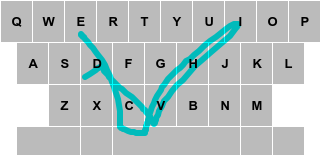
\includegraphics[width=\w]{imgs/vvr5s7lo8lhibvfm37q7vag4mb-advice-0.png}}\hfill
    \subfloat[\texttt{manchester}]{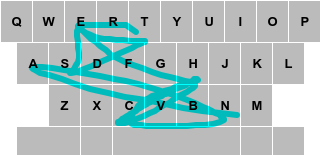
\includegraphics[width=\w]{imgs/vvr5s7lo8lhibvfm37q7vag4mb-manchester-0.png}}\hfill
    \subfloat[\texttt{tomorrow}]{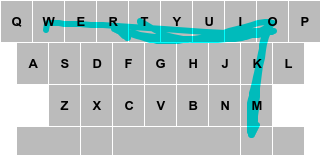
\includegraphics[width=\w]{imgs/vvr5s7lo8lhibvfm37q7vag4mb-tomorrow-0.png}}\\
    \subfloat[\texttt{wellcare}]{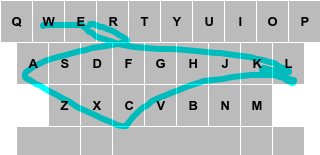
\includegraphics[width=\w]{imgs/vvr5s7lo8lhibvfm37q7vag4mb-wellcare-0.png}}\hfill
    \subfloat[\texttt{download}]{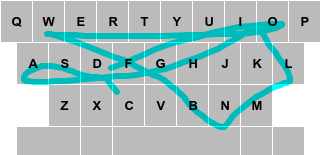
\includegraphics[width=\w]{imgs/vvr5s7lo8lhibvfm37q7vag4mb-download-0.png}}\hfill
    \subfloat[\texttt{twitter}]{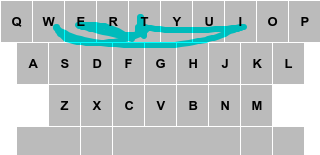
\includegraphics[width=\w]{imgs/vvr5s7lo8lhibvfm37q7vag4mb-twitter-0.png}}

    \caption{Examples of swiped word trajectories.}
    \label{fig:swipe-examples}
\end{figure*}

Swiping performance has been researched in small-scale experiments~\cite{Reyal2015},
in large-scale studies as one of many text methods~\cite{Palin19},
or using proprietary, undisclosed datasets~\cite{Quinn18}.
Collecting such data is challenging, because
most mobile keyboards are vendor-locked and do not offer an API for collecting such data~\cite{Leiva21_swipe}.

Until now, there was no public swiping dataset where researchers could access raw movements dynamics
such as the gesture path drawn on top of the keyboard or the time lapsed between consecutive swiped keys.
Recently, Leiva et al.~\cite{Leiva21_swipe} released \rev{``How We Swipe''},
the largest dataset (over 1,300 participants)
for conducting research on mobile swiping together with first observations of correlates of typing performance.
Large-scale analyses of mobile interaction are relatively rare
and mostly undertaken by commercial organizations and mobile vendors that ship soft keyboards.
There are notable exceptions~\cite{Buschek18, Henze12, Dhakal18, Palin19} but they did not investigate swiping behavior.

In this work we analyse the dynamics of swiping trajectories to model and predict different demographic and behavioral correlates,
including age, gender, nationality, English level, swiping familiarity, swiping hand, swiping finger, and dominant hand.
In total, we trained 200+ different classifiers with 30 different hyperparameter variations for each predicted target.
We found that swipe trajectories actually carry information about demographic and behavioral correlates.
To the best of our knowledge, we are the first to perform this analysis in this kind of data.

The rest of this article is organized as follows. In \autoref{sec:related_work}, we present a comprehensive overview of related works in shape writing and user profiling from demographic and behavioral movement data. In \autoref{sec:experiments}, we present the dataset we have analyzed and the methodology we have followed. In \autoref{sec:discussion} we discuss the results of our experiments. In \autoref{sec:limitations}, we present a comprehensive summary highlighting limitations and future research directions. Finally, \autoref{sec:conclusion} closes this article with a summary of the main findings.


%% ============================================================================
\section{Related Work}
\label{sec:related_work}
%% ============================================================================

%% What has been done before? Why is it not good enough?
%% We need to discuss at least 10 related papers.

Invented by Zhai and Kristensson in 2003~\cite{Zhai03},
swiping has become a widely adopted text entry method on mobile devices.
It well suits touch-based interaction, and provides a high typing speed
since it relaxes the requirement of precisely acquiring each (small) key on a soft keyboard.
To date, this text entry method is supported by major commercial soft keyboards
including Google's Gboard, Microsoft' SwiftKey, and iOS's built-in keyboard on iPhones.

The research community has carried out a large amount of research on swiping techniques.
For example, swiping has been extended to support mid-air text entry~\cite{Markussen:2014:VMW}, eyes-free input~\cite{zhu2019sfree}, ring-based input~\cite{gupta2019rotoswype}, phone-tilting based input~\cite{yeo2017investigating}.
In addition to text entry, swiping has also been extended to support command input~\cite{kristensson2007command, alvina2017commandboard, cui2019hotstrokes},
by gesturing a shortcut related to the command name.
Such a method shows advantages in learnability compared with hotkey-based command input~\cite{cui2019hotstrokes}.

There is a large body of work that demonstrates that our digital footprints,
including e.g. the websites we visit or the text we enter in social media,
may help derive personally identifiable information like gender, age, location, or even political orientation.
Existing literature related to online privacy provides insights around topics such as
information leakage while surfing the web using desktop computers~\cite{Starov_2016}
or mobile devices~\cite{Leung_2016}.
In the following we discuss related work aimed at exploiting this information
in the context of human movement data, such as handwriting and gesturing,
since they are the closest work to swiping.
% Again, we emphasize on the lack of public datasets about swiping until now,
% which has made not possible this kind analysis before.


\subsection{Biometrics Prediction from Movement Data}

%% https://luis.leiva.name/web/docs/papers/handwriting-biometrics-icpr2020-preprint.pdf
Leiva et al.~\cite{Leiva20_biometrics} showed that accurate detection of human movements
has more to do with \emph{how} users write, rather than \emph{what} they write.
They concluded that it is better to use recurrent models than convolutional models for biometric classification,
as recurrent models capture the inherent movement dynamics.
However, they only explored one shallow architecture,
based on Bidirectional Gated Recurrent Unit (BiGRU) cells,
in the context of binary classification of human vs. fake handwriting.
Therefore, it is unclear what design choices over the different hyperparameters
(e.g. number of hidden layers, type of recurrent cell, number of hidden units, learning rates, etc.)
may affect classification performance.
In this work we perform an exhaustive investigation in this regard.

%% Leiva et al.~\cite{Leiva21_swipe} mentions previous work about text entry:
%% https://luis.leiva.name/web/docs/papers/shapewriting-mobilehci2021-preprint.pdf

%% Leiva et al.~\cite{Leiva21_privacy} provide an extensive literature review of biometric-like classifiers:
%% https://luis.leiva.name/web/docs/papers/mouseprivacy-chiir2021-preprint.pdf
Leiva et al.~\cite{Leiva21_privacy} showed that our mouse movements may reveal who we are.
They developed a computational model based on BiGRU cells and were able to classify the age and gender of the users
with reasonable precision (near 70\%) using a few lines of code.
%These results suggest that our digital privacy is at risk,
%since today it has become trivial to acquire mouse movements unobtrusively and at large scale.
%Furthermore, developing sophisticated classifiers is easier than ever thanks to libraries like Scikit-learn, Tensorflow, or Pytorch.
Recent work by White et al.~\cite{White18} and Gajos et al.~\cite{Gajos20}
could detect neurodegenerative disorders from mouse cursor movements,
showing how our ``digital phenotypes'' could be used as adjunctive screening tools.

Chen et al.~\cite{Chen_2001} were the first to notice a strong relationship between gaze position and cursor position during web browsing.
Mueller and Lockerd~\cite{Mueller01_cheese} investigated the use of mouse tracking to visualize and (manually) infer the users' interests.
Since then, researchers have noted the utility of mouse cursor analysis
as a low-cost and scalable proxy of eye gaze~\cite{Huang12_search, Huang12_align, Navalpakkam13_layout}.
Several works have investigated closely the utility of mouse cursor data in web search~\cite{Arapakis16_dds, Chen17_satisfaction, Liu15_opinions}
and web page usability evaluation~\cite{Arroyo06_usab, Atterer06_move, Leiva11_adapt},
two of the most prominent use cases of this technology.
Mouse biometrics is another active research area that has recently shown how to identify an individual
by analyzing their mouse movements in controlled settings~\cite{Kratky18_biom, Lu17_biom}.
This is the research line we focus on in this work.

Objective measurements of attentional processes are increasingly being used to explain or predict user behavior.
% Early mouse cursor tracking systems began by logging click events only (coordinates and timestamp)
% and using these events to assess what information users were interested in.
% However, it was soon realized that click data provide an incomplete picture of user interaction.
A mouse click is often preceded by several interactions such as scrolling, hovers, movements, etc.
and thus can lead to a better overall understanding of the user's thought process.
%
In what follows, we review research efforts that have focused on mouse cursor analysis
to infer user interest, visual attention, emotions, and demographic variables like gender or age, on a desktop setting.
We hypothesize that swiped word trajectories carry the same rich information about the user.

\subsection{Inferring User Interest}
\label{sec:interest}

For a long time, commercial search engines have been interested in how users interact with Search Engine Result Pages (SERPs),
to anticipate better placement and allocation of ads in sponsored search or to optimize the content layout.
Early work considered simple, coarse-grained features derived from mouse cursor data
to be surrogate measurements of user interest~\cite{Claypool01_iii, Shapira06_ii}.
Follow-up research transitioned to more fine-grained mouse cursor features~\cite{Guo08_query, Guo10_buy}
that were shown to be more effective.
These approaches have been directed at predicting open-ended tasks
like search success~\cite{Guo12_success} or search satisfaction~\cite{Liu15_opinions}.
In a similar vein, Huang et al.~\cite{Huang12_search, Huang11_clicks}
modeled mouse cursor interactions and extended click models to compute more accurate relevance judgements of search results.
Mouse cursor position is mostly aligned to eye gaze,
especially on SERPs~\cite{Guo12_rel, Speicher13_rel},
and that can be used as a good proxy for predicting good and bad abandonment~\cite{Diriye12_leaving}.

\subsection{Inferring Visual Attention}
\label{sec:attention}

Mouse cursor tracking has been also used to survey the visual focus of users in sponsored search,
thus revealing valuable -- and at the same time sensitive -- information
regarding the distribution of user attention over the various SERP components.
Despite the technical challenges that arise from this analysis,
previous work has shown the utility of mouse movement patterns
to measure within-content engagement~\cite{Arapakis14_news}
and predict reading experiences~\cite{Arapakis14_gestures, Hauger11}.
Lagun et al.~\cite{Lagun14_motifs} introduced the concept of motifs,
or frequent cursor subsequences, in the estimation of search result relevance.
Similarly, Liu et al.~\cite{Liu15_opinions} applied the motifs concept to SERPs
and predicted search result utility, searcher effort, and satisfaction at a search task level.
Boi et al.~\cite{Boi2016} proposed a method for predicting whether the user is looking at the content pointed by the cursor,
exploiting the mouse cursor data and a segmentation of the contents in a web page.
Lastly, Arapakis et al.~\cite{Arapakis16_dds, Arapakis20_ppa}
investigated user engagement with direct displays on SERPs
and provided further evidence that supports the utility of mouse cursor data
for measuring user attention at a display-level granularity.

\subsection{Inferring Emotional State}
\label{sec:emotion}

Although the connection between mouse cursor movements and the underlying psychological states has been a topic of research
since the early 90s~\cite{Accot97_fitts, Card87_mouse},
some studies have investigated the utility of mouse cursor data for predicting the user's emotional state.
For example, Zimmermann et al.~\cite{Zimmermann2003} investigated the effect of induced affective states
on the motor-behavior of online shoppers and found that the total duration of mouse cursor movements
and the number of velocity changes were associated to the experienced arousal.
Kaklauskas et al.~\cite{Kaklauskas2009}
created a system that extracts physiological and motor-control parameters
from mouse cursor interactions and then triangulated those with psychological data taken from self-reports,
to analyse correlations with users' emotional state and labour productivity.
In a similar line, Azcarraga et al.~\cite{Azcarraga12_brain} combined electroencephalography signals and mouse cursor interactions
to predict self-reported emotions like frustration, interest, confidence and excitement.
Yamauchi et al.~\cite{Yamauchi13_anxiety} studied the relationship between mouse cursor trajectories and generalized anxiety in human subjects.
Lastly, Kapoor et al.~\cite{Kapoor07_frustration} predicted whether a user experiences frustration, using an array of affective-aware sensors.

\subsection{Inferring Demographics}
\label{sec:demographic_attributes}

Yamauchi et al.~\cite{Yamauchi2014} examined the extent to which mouse cursor movements can help identify the gender
and the experienced feelings of users who were watching short film clips.
Although this work provides early evidence on the utility of mouse cursor data for advanced online user profiling,
it suffers from certain limitations that we address in this work.
First, the experimental setting has limited generalizability,
since the adopted perception task is not very well connected
to typical activities that users perform online, such as web search.
Second, the data used in their predictive modeling task include multiple samples per participant
randomly assigned to the training and test data partitions,
hence there may be information leakage that artificially inflated model performance.
In our analysis, we limit the training samples to exactly one mouse cursor trajectory per participant
and test our models on unseen individuals.

Kratky et al.~\cite{Kratky16_demographics} recorded mouse cursor movements in an e-commerce website
and engineered a set of meta-features to predict the user gender and age group.
Their classifier was trained on several days of data per participant.
Although the training and test collections had disjoint sets of participants,
it was stated that the reported results were overly optimistic
since researchers could not verify their ground-truth data~\cite{Kratky16_demographics}.
In contrast, as discussed later,
our dataset was collected from high-quality crowdworkers
so we are confident that the ground-truth information is correct.

In a similar vein, Pentel et al.~\cite{Pentel2017} used data from six different external sources,
including e.g., keystroke data and feedback questionnaires,
and handcrafted features proposed in earlier works~\cite{Claypool01_iii, Diriye12_leaving, Shapira06_ii}
to train predictive models that could identify the users' age and gender.
However, because their approach relies mainly on ad-hoc data,
it is less scalable and more difficult to implement than the approach we propose in this paper,
which takes as input \emph{raw} mouse cursor data.
Moreover, Pentel et al. reported optimistic performance scores,
which may be due to information leakage across data partitions,
and omit important classification metrics such as precision, recall, and AUC.
To account for their modeling approach, as well as that proposed by Kratky et al.~\cite{Kratky16_demographics},
we implement the same classifier and test it in our setting.

\subsection{Summary}

There is a vast research literature about modeling user behavior using movement data.
How we move our mouse provides a surrogate signal for gaze fixation,
and therefore reveals our focus of attention,
which can be used to learn \emph{latent} interests.
However there is no previous work in this regard using swipe trajectories.
This is because of the lack of public datasets, which are difficult to collect in practice.
Fortunately, Leiva et al.~\cite{Leiva21_swipe} have recently released a swiping dataset
that enables researchers to create sophisticated Machine Learning models.
To the best of our knowledge, we are the first to tap into this dataset
to create different biometric-related classifiers.


%% ============================================================================
\section{Experiments}
\label{sec:experiments}
%% ============================================================================

Based on the research literature,
we hypothesize that cognitive and motor control mechanisms are embodied
and reflected, to some extent, in swipe trajectories.
If our classification results prove to be better than random,
this work will open a new research avenue for advanced user profiling.

\subsection{Dataset}

%% TODO: Plot the distribution of each target variable, similar to Fig.4 in the "How We Swipe" paper.
%% https://luis.leiva.name/web/docs/papers/shapewriting-mobilehci2021-preprint.pdf

The swiping dataset we used in this study is publicly available at \url{https://osf.io/sj67f/}.
It covers both movement-level and task performance-level data,
and was collected in a crowdsourcing study using a JavaScript-based virtual QWERTY \rev{soft} keyboard.
The dataset comprises 100K+ English words swiped by 1,338 users.
Each word was swiped in the context of either a memorable sentence,
drawn from the EnronMobile phrase set~\cite{Vertanen11_enron},
or a random 4-words sentence, drawn from Google's Trillion Word Corpus\footnote{\url{https://github.com/first20hours/google-10000-english}}
and the Forbes 2019 Global 2000 list.\footnote{\url{https://www.forbes.com/global2000/}}
All words are lowercased with no punctuation symbols.

Swipe logs include the following information:
event name (e.g. \texttt{touchstart}, \texttt{touchmove}),
event timestamp,
\texttt{x} and \texttt{y} coordinates,
touch radius,
and rotation angle, where available.
The logs also include the keyboard size, the prompted word, and whether it was swiped correctly or not.
We deliberately ignore the wrongly swiped words,
as they were clear outliers, as described in the dataset~\cite{Leiva21_swipe}.
There are 11,295 unique words correctly swiped which we consider for analysis.
%
Additionally, the dataset provides the following user metadata:
swipe familiarity, age, gender, nationality, browser language,
device pixel ratio, screen size (height and width), English level,
dominant hand, swipe hand, swipe finger, and mobile vendor.
In this paper, we predict all the biometric-related variables:
swipe familiarity, age, gender, nationality, English level, dominant hand, swipe hand, and swipe finger.\\

For the task of training our classifiers, we performed a light preprocessing on the dataset.
First, we iterated through the 1,338 user logs and gathered the raw trajectories of \texttt{mousemove} $x,y$ coordinates and associated timestamps $t$
for each of the individual correctly swiped words.
Each raw trajectory has the following format:
$(x,y,t)_1, \dots, (x,y,t)_n$ where $(x,y,t)_i = (x_{i}, y_{i}, t_{i})$.
Then, we computed the offsets of the raw points,
as it makes our sequence models scale-invariant and independent of the device's screen size:
$(\Delta x, \Delta y, \Delta t)_i = (x_{i} - x_{i+1}, y_{i} - y_{i+1}, t_{i} - t_{i+1})$.
Eventually, our final dataset contains a total of 94,841 swiped word trajectories from 1,308 unique participants.


\subsection{Predictive Targets}
\label{sec:targets}

\autoref{fig:distributions} shows the class distributions of the targets we set to predict in this article.
From the figures we can see that some targets are more imbalanced than others.
This can potentially bias to our sequence classifiers,
so we created splits of the data as balanced as possible, as explained next.

\begin{figure}[!ht]
\centering
\def\w{0.24\linewidth}

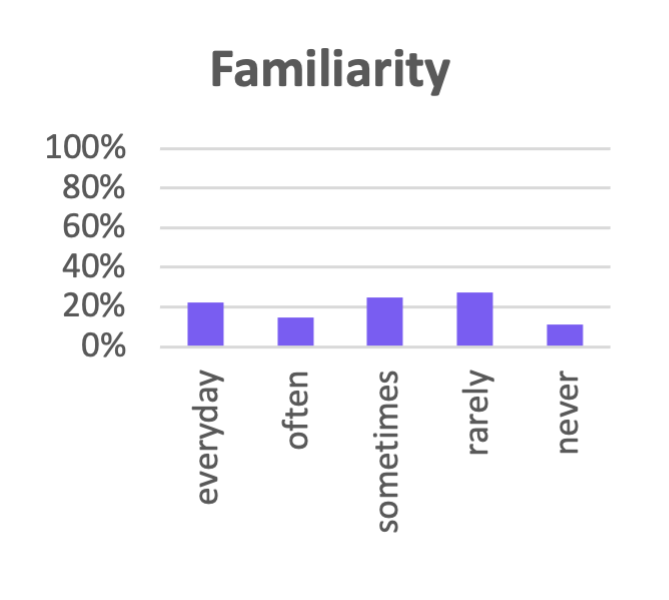
\includegraphics[width=\w]{figures/familiarity_distribution.png} \hfill
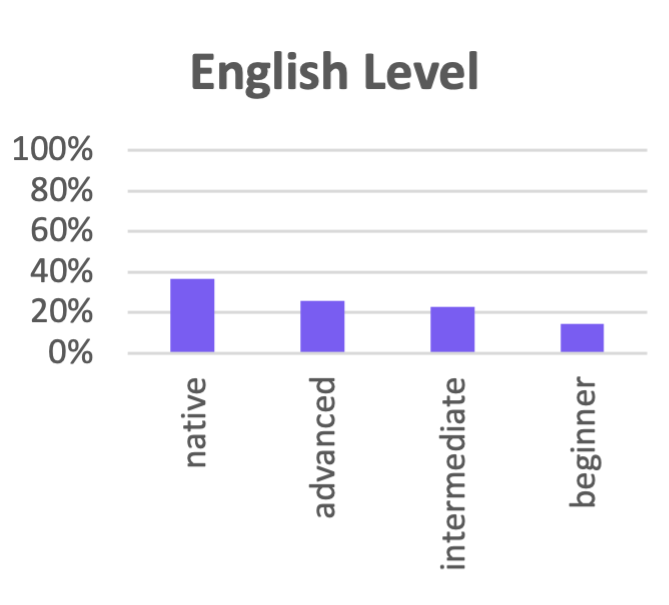
\includegraphics[width=\w]{figures/english_distribution.png} \hfill
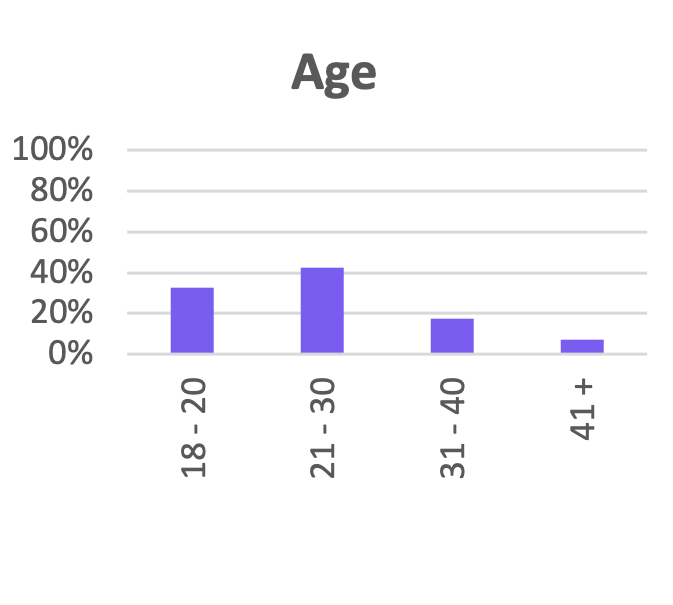
\includegraphics[width=\w]{figures/age_distribution.png} \hfill
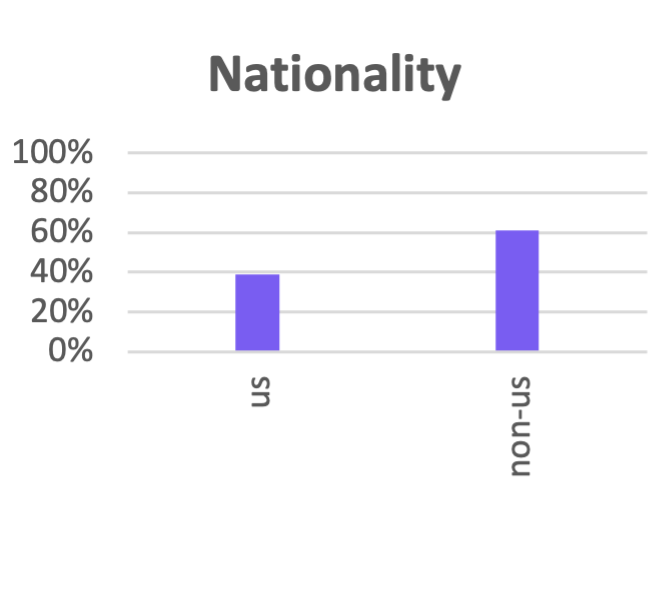
\includegraphics[width=\w]{figures/nat_distribution.png} \\
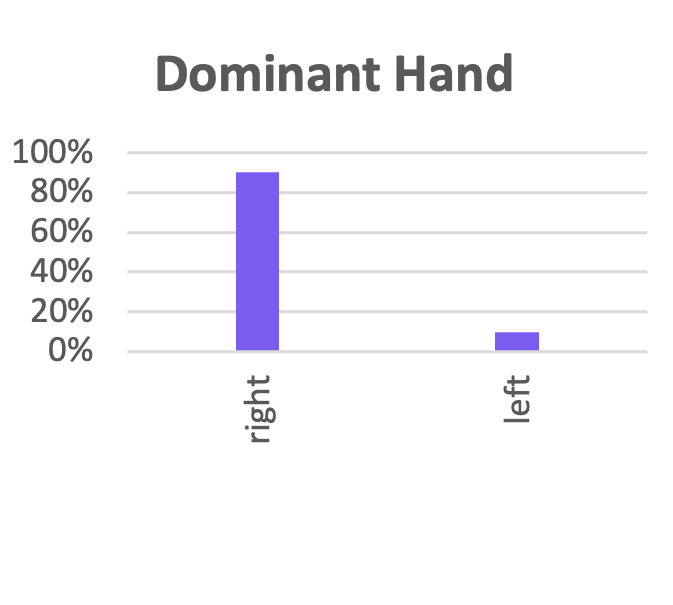
\includegraphics[width=\w]{figures/dom_distribution.png} \hfill
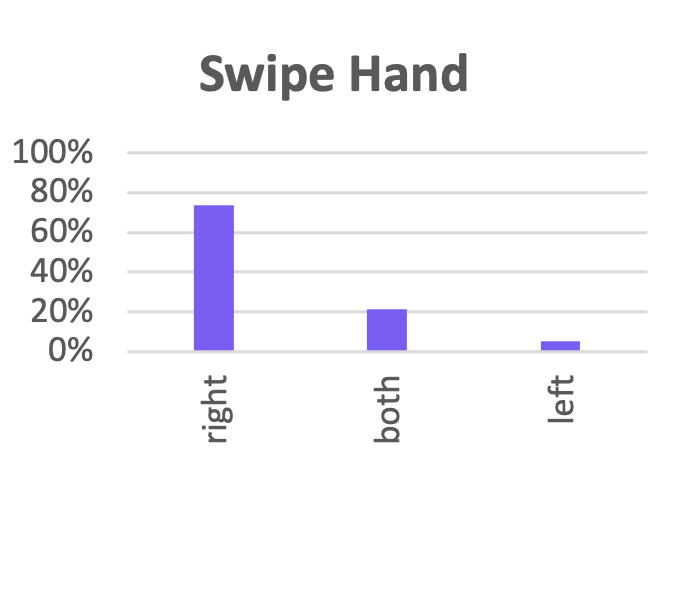
\includegraphics[width=\w]{figures/hand_distribution.png} \hfill
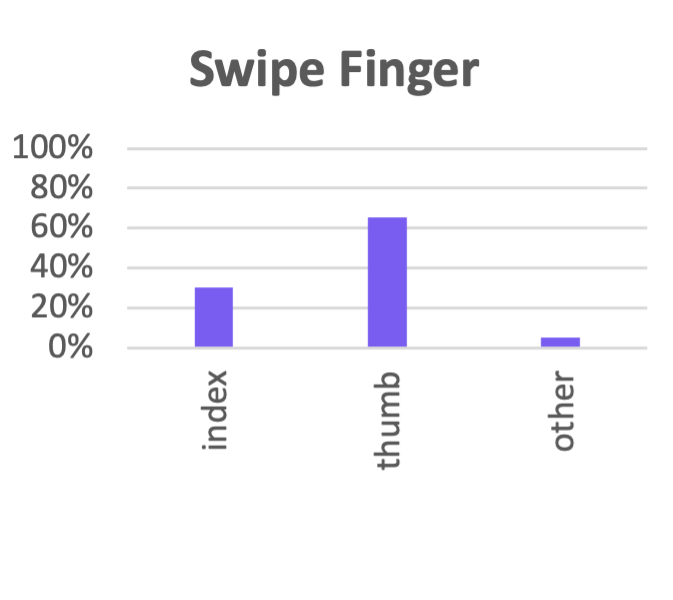
\includegraphics[width=\w]{figures/finger_distribution.png} \hfill
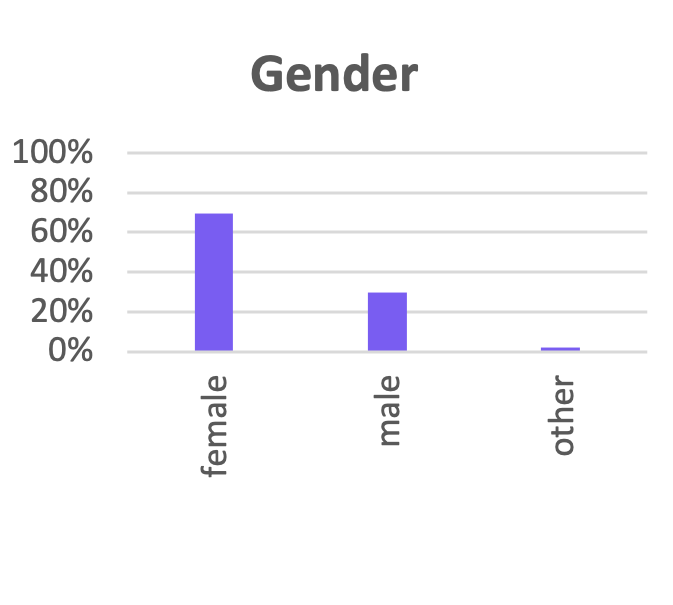
\includegraphics[width=\w]{figures/gender_distribution.png} \\

\caption{Targets and their class distributions in the original swiping dataset.}
\label{fig:distributions}
\end{figure}

The \textbf{familiarity} target describes how well a user is used to swiping and contains 5 classes in the original dataset:
``everyday'' (22\%), ``often'' (15\%), ``sometimes'' (25\%), ``rarely'' (27\%) and ``never'' (11\%).
By looking at the class distributions, we can see that the class ``often'' and ``never'' are twice as small as the other classes.
Therefore, we merged the ``often'' class with ``everyday'' and the ``never'' class with ``rarely''.
Eventually we ended up with 3 classes for our experiments: ``everyday'' (37\%), ``sometimes'' (25\%) and ``rarely'' (38\%).

The \textbf{English level} target has 4 classes in the original dataset:
``native'' (34\%), ``advanced'' (27\%), ``intermediate'' (24\%), and ``beginner'' (15\%).
In this case the class distributions are fairly balanced except ``beginner'',
however the class semantics are important to preserve in this case.
Leiva et al.~\cite{Leiva21_swipe} reported that ``intermediate'' and ``beginner'' English speakers
were significantly slower and committed more errors than any of the other users,
therefore we did not modify the original class distributions for the English level target.

The \textbf{age} target has 4 classes in the original dataset:
``youth'' (18--20 years, 33\%),
``young'' (21--30 years, 42\%),
``adult'' (31--40 years, 18\%)
and ``senior'' (41+ years, 7\%).
Since these class distributions are rather imbalanced,
we redefine the age brackets as follows:
``youth'' (18--20 years, 33\%),
``young'' (21--28 years, 37\%),
``adult'' (29+ years, 30\%).

% \begin{figure*}[h]
%     \centering
%     \def\w{0.45\textwidth}
%     \subfloat[\text{Age}]{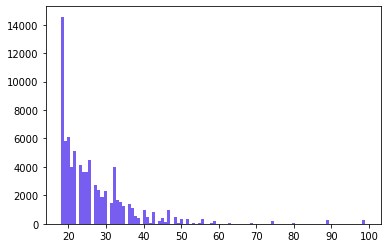
\includegraphics[width=\w]{figures/age.png}}
%     \hspace{1cm}
%     \subfloat[\text{Sequence Length}]{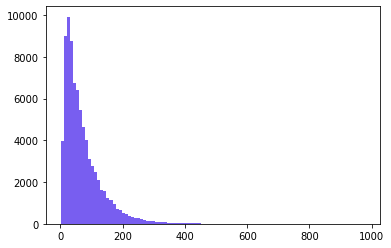
\includegraphics[width=\w]{figures/sequence_length.png}}
%     \caption{Distributions for age and sequence length}
%     \label{fig:age-seq}
% \end{figure*}

The \textbf{nationality} target describes whether a user is a US citizen,
given that US users were over-represented in the original dataset.
The class distributions are: 39\% ``US'' and 61\% ``non-US'' users.
Since there are two classes, we did not modify the original class distributions.

The \textbf{dominant hand} target describes the hand the user uses the most.
The class distributions are: 90\% ``right-handed'' and 10\% ``left-handed'' users.
Since there are two classes, we did not modify the original class distributions.

The \textbf{swipe hand} label describes if the user likes to use the right, left, or both hands to swipe.
The original dataset has 3 classes: 74\% ``right hand'', 21\% ``both hands'', and 5\% ``left hand''.
Due to their significant difference in size compared to the right hand class,
we decided to merge the ``left hand'' and ``both hands'' classes.
Eventually we ended up with 2 classes for our experiments:
``right hand'' (74\%), ``other hand'' (26\%).

The \textbf{swipe finger} label describes which finger the user prefers to swipe with.
The original dataset has 3 classes: ``index finger'' (65\%), ``thumb'' (30\%), and ``other finger'' (5\%).
Given that the latter class is substantially smaller that the rest,
% we left it out and rebalance the 2 final classes: ``index finger'' (69\%) and ``thumb'' (31\%).
we left it out and consider 2 classes in our experiments: ``index finger'' and ``thumb''.

The \textbf{gender} target includes ``female'' (69\%), ``male'' (30\%), and ``other'' (1\%).
Given that the latter class is substantially smaller that the rest,
% we left it out and rebalance the 2 final classes: ``female'' (70\%) and ``male'' (30\%).
we left it out and consider 2 classes in our experiments: ``female'' and ``male''.

We can see that, even after this careful class redistribution procedure,
some of our targets still have notable imbalanced classes.
To address this challenge we used cost-sensitive models via class weighting,
as described in the next section.


\subsection{Model Architectures}

%% What models were selected? Diagram of the architectures: input layer -> recurrent layer(s) -> dropout -> dense layer -> output layer
%% What are their characteristics? Who do they work? Add diagrams of RNN/LSTM/GRU cells.
%% What hyperparameters were varied? e.g. num hidden layers, num hidden units, etc.

%% How the models were trained? optimizer (Adam), batch size, early stopping, etc.
Since swipe trajectories are sequences of coordinates, we have chosen to train sequence models.
Sequence models are Machine Learning models to handle sequential data,
where each observation is dependent or contextually related to the previous one, such as text streams, audio, time-series data, etc.
Recurrent Neural Networks (RNN) are by far the most popular algorithms used in sequence models.
RNNs consist of standard recurrent cells, shown in \autoref{fig:rnn-model}.

The typical feature of the RNN cell is a cyclic (or \emph{loop}) connection,
which enables the model to update the current state based on past states and current input data.
Formally, the standard recurrent cell is defined as follows:
%
\begin{align}\label{eq:rnn}
    h_j &= \Phi(W_h h_{j-1} + W_z z_j + b) \\
    o_j &= h_j
\end{align}
%
where
%
$z_j = (x,y,t)_j$ denotes the $j$th vector of the input signal
$\mathbf{z} = (x,y,t)_{j = 1, \cdots, |z|}$ at timestep $j$
(i.e., the index at which a point coordinate has happened),
$h_j$ is the hidden state of the cell,
and $o_j$ denotes the cell output, respectively;
$W_h$ and $W_z$ are the weight matrices;
$b$ is the bias of the neurons;
and $\Phi$ is an activation function.

\begin{figure}[!ht]
\centering
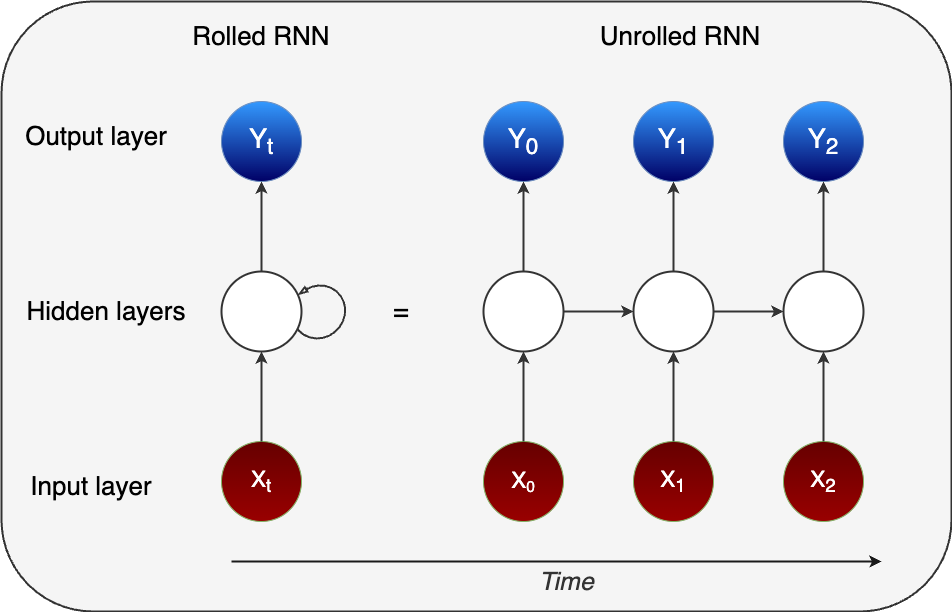
\includegraphics[width= 0.5\textwidth]{plots/RNN.png}
\caption{Standard RNN architecture.}
\label{fig:rnn-model}
\end{figure}

Standard recurrent cells have achieved success in many sequence learning problems
such as natural language processing~\cite{Sutskever14}, action recognition~\cite{Du18}, or image captioning~\cite{Mao15}.
However, the standard recurrent cells are not capable of handling long-term dependencies.
To solve this issue, the LSTM and GRU cells were developed~\cite{Hochreiter97_lstm, Cho14_gru}.
They improve the capacity of the standard recurrent cell by introducing different gates,
which we briefly describe as follows.

On the one hand, the LSTM cell is defined as follows:
%
\begin{align}
        G_i &= \sigma(W_u [ h_{j-1}, z_j ] + b_i) \\
        G_f &= \sigma(W_f [ h_{j-1}, z_j ] + b_f) \\
        G_o &= \sigma(W_o [ h_{j-1}, z_j ] + b_o) \\
        c_j &= \rev{G_i} \odot \tilde{c}_j + G_f \odot c_{j-1} \\
\tilde{c}_j &= \Psi(W_c [ h_{j-1}, z_j ] + b_c) \\
        h_j &= G_o \odot \Psi(c_j)
\end{align}
%
where
$c_j$ is a hidden state responsible for the long-term memory,
\rev{$\tilde{c}_j$ is a candidate state responsible for controlling the cell-state data,}
$W_*$ are weight matrices,
$b_*$ are biases,
$G_*$ denote cell gates (i: input, f: forget, o: output),
and $\Psi$ and $\sigma$ are activation functions. %(hyperbolic tangent and sigmoid, respectively).
The $\odot$ operator denotes the Hadamard (element-wise) product.

As noted, the LSTM has two kinds of hidden states~\cite{Jozefowicz15}:
a ``slow'' state $c_j$ that keeps long-term memory, % to overcome the vanishing gradient problem,
and a ``fast'' state $h_j$ that makes decisions over short periods of time.
The forget gate $G_f$ can decide what information will be thrown away from the cell state.
In practice, the activation functions $\Psi$ and $\sigma$ are hyperbolic tangent and sigmoid, respectively,
however other non-linear functions have been promoted in the research literature;
see the next section for a brief discussion.

On the other hand, the GRU cell is defined as follows:
\begin{align}
        G_u &= \sigma(W_u [ h_{j-1}, z_j ] + b_u) \\
        G_r &= \sigma(W_r [ h_{j-1}, z_j ] + b_r) \\
\tilde{c}_j &= \Psi(W_c [G_r \odot h_{j-1}, z_j ] + b_c) \\
        h_j &= G_u \odot \tilde{c}_j + (1 - G_u) \odot h_{j-1}
\end{align}
where the forget and input gates of the LSTM cell are now combined into a single update gate $G_u$.
A reset gate $G_r$ controls which parts of the state get used to compute next cell state.
The LSTM and GRU architectures are presented in figure \autoref{fig:LSTM_GRU model}.
As it can be observed, GRU controls the flow of information like the LSTM cell,
but without having to use memory (the forget and output gates in LSTM):
the full state vector is output at every time step.
Furthermore, performance-wise the GRU cell is on par with the LSTM in many problems~\cite{Chung14,Dey17}
but it is computationally more efficient because of its less complex structure.
Therefore, our classifier uses GRU cells for its RNN layer. % as in our previous work~\cite{Leiva20_icpr}.


\begin{figure}
     \centering
     \begin{subfigure}[b]{0.45\textwidth}
         \centering
         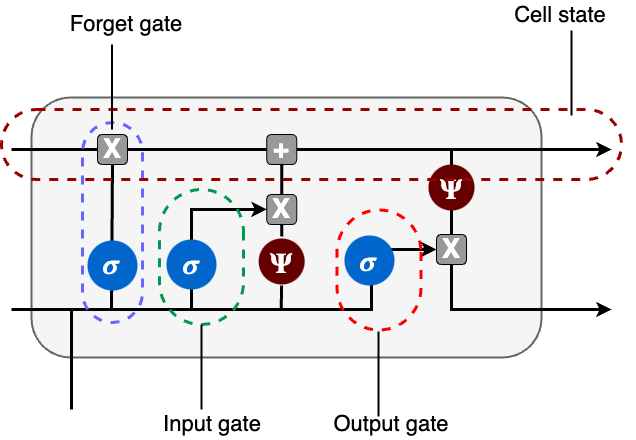
\includegraphics[width=\textwidth]{plots/LSTM.png}
         \caption{LSTM cell.}
         \label{fig:lstm-model}
     \end{subfigure}
     \hfill
     \begin{subfigure}[b]{0.45\textwidth}
         \centering
         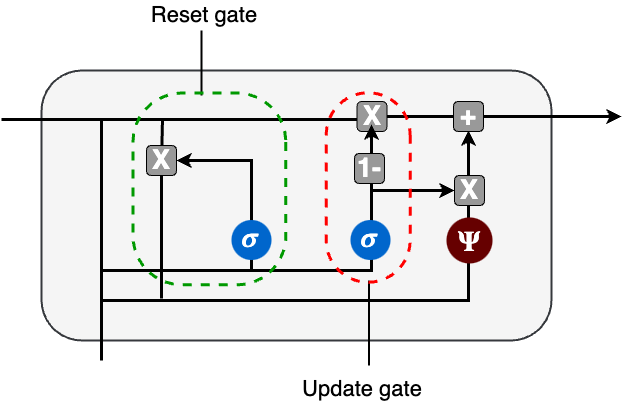
\includegraphics[width=\textwidth]{plots/GRU.png}
         \caption{GRU cell.}
         \label{fig:gru-model}
     \end{subfigure}
    \caption{Overview of the LSTM and GRU cells.}
    \label{fig:LSTM_GRU model}
\end{figure}

As can be observed, GRU controls the flow of information like the LSTM cell,
but without having to use memory (the forget and output gates in LSTM):
the full state vector is output at every time step.
Furthermore, performance-wise the GRU cell has been shown to be on par with the LSTM in many problems~\cite{Chung14,Dey17}
while at the same time being computationally more efficient because of its less complex structure.
It remains unclear, however, what would be the best RNN-based architecture configuration
(e.g. type of cell, number of layers, number of neurons, etc.)
for predicting demographic and behavioral correlates from swipe trajectories.
Therefore, we study what is the most suitable configuration.

The hyperbolic tangent activation function is applied in every recurrent layer,
since recurrent neural networks do not only get gradients from lower layers but also from previous timesteps.
The derivatives of tanh are larger than the other activation functions such as sigmoid or swish.
Thus, the cost function is minimized faster by using the hyperbolic tangent activation function.
It has a normalized range from -1 to 1 and the output is symmetric around 0 which leads to faster convergence.
Formally:
%
\begin{equation}\label{eq:tanh}
  \text{tanh(z)} = \frac{e^{z} - e^{-z} }{e^{z} + e^{-z} }
\end{equation}

Finally, the classification rule of all the classifiers we trained is defined by:
%
\begin{equation}\label{eq:classification-rule}
\hat{z} = \text{softmax}(W_z \odot h_j + b_z)
\end{equation}
%
where $\text{softmax}(\mathbf{v})$ is the softmax function,
which normalizes the output of the last network layer
(denoted as $\mathbf{v}$ for the sake of simplicity)
to a probability distribution over the predicted output classes $K$:
%
\begin{equation}\label{eq:output}
  \text{softmax} ( \mathbf{v} )_{i} = \frac{e^{v_i}}{\sum _{j=1}^{K} e^{v_j}}
\end{equation}
%
for $i = \{1, \dots, K\}$ and $\mathbf{v} = (v_1, \dots, v_K)$. \\


\subsection{Methodology}

Neural networks require inputs with the same shape and size, at least within the same batch.
However, the trajectories in the swiping dataset have varying sequence lengths \rev{(Mean=72, StDev=64)}.
%ranging from 1 (min length) to 979 points (max length).
Thus, we need to apply padding and truncation to the sequence trajectories in order to ensure equally-sized lengths.
We chose 200 points as our maximum sequence length, based on the data distribution,
thus all sequences were padded or truncated to this maximum capacity.

For the data split ratio, we \rev{randomly} used 60\% for the training set, 20\% for the validation set
and the remaining 20\% for the testing set.
\rev{Each model was trained and evaluated on the very same data partitions.
The testing partition is held out exclusively for model evaluation, as it represents unseen data
and is therefore a more challenging but also a more realistic scenario.
}
We chose to work with the Adam optimizer since it is an algorithm for efficient stochastic optimization
that only requires first-order gradients with little memory requirement~\cite{Adam}.
The loss function to minimize is sparse categorical cross-entropy,
since our task is a multi-class classification problem with $C \geq 2$ classes.

\subsubsection{Model Hyperparameters}

We conducted a systematic analysis regarding which architecture hyperparameters affect model performance.
The architecture choices include the type of layer (RNN, LSTM or GRU),
whether bidirectional or not, number of hidden neurons, number of hidden layers, and optimizer's learning rate.

In bidirectional models, the input flows in both directions
such that every component of an input sequence is able to use the information from both the past and present.
The model adds for each recurrent layer another recurrent layer with the reversed information flow.
The outputs from forward and backward layers are combined by concatenating them.
% The disadvantage of bidirectional models is that they are slower since they require more time for training.

The learning rate controls how quickly a neural network model adapts to a problem.
By choosing smaller learning rates, the model might result in a long training or might get stuck in the process
since the changes made to the weights each update are smaller.
On the other hand, the model might converge too fast to a sub-optimal solution by choosing larger learning rates.
We experimented with learning rate (LR) 10$^{-1}$, 10$^{-2}$, 10$^{-3}$, 10$^{-4}$ and 10$^{-5}$, 5 variations in total.
\rev{
Note that LR higher than 10$^{-1}$ is unlikely to work because of the Robbins-Monro condition:
the more LR approaches 1, the less room for the model to learn from backpropagation.
Further, when LR $> 1$, stochastic gradient descent is not guaranteed to converge to a minimum~\cite{Ranganath14}.
}

We tested the performance of the different layer types (RNN, BiRNN, LSTM, BiLSTM, GRU and BiGRU), 6 variations in total for each target.
%We tested how the number of hidden layers as well as the number of hidden neurons impacts our model's performance.
The number of hidden layers we tested range from 1 to 4 layers in our model architectures, 4 variations in total.
The number of hidden units range from 10 to 150, with a step size of 10, 15 variations in total. % i.e. 10, 20, ..., 150 units
Eventually, we tested 30 different hyperparameter variations for each predicted target,
totalling a number of 240 different trained classifiers.

%%%While training, the model underfits if we train the model too little. On the other hand, the model overfits the train set and perfoms poorly on the test set if we train too long.  We decided therefore to apply early stopping in the training of our neural network. Thus, our model trains on the train set until its performance on the validation set starts to degrade i.e. generalization error starts to increase.

\subsubsection{Model Regularization}

We use two popular regularization techniques to prevent overfitting and make our classifiers more generalizable: Dropout and Early Stopping.
Dropout removes neurons at random during training,
to force different connection paths between neurons
and thus avoid the model to take shortcuts (like creating spurious correlations between inputs and outputs).
We used Dropout with 0.15 probability in all RNN layers.
Early Stopping stops training when no further improvements over a given metric (e.g. classification accuracy, validation loss) are made.
We set 40 epochs of patience for Early Stopping while monitoring the F1 score,
i.e. if the model does not improve the F1 score over the validation data in 40 consecutive epochs,
training stops and the best model weights are retained.
The maximum number of training epochs is set to 500 and batch size is set to 32 trajectories.

As discussed in the previous section, our class distributions are imbalanced for most of the targets.
To address this challenge we used cost-sensitive models via class weighting.
The idea is to give all classes equal importance on gradient updates,
regardless of how many samples we have from each class in the training data.
This prevents models from predicting the more frequent class more often just because it is more common.
Instead, class weighting forces models to learn a more apt representation of each class.

%%%to assign different weights to different misclassification errors. More precisely, we want to force the model to pay more attention to the minority classes during training by making the weight of misclassification relatively high compared to the weight of misclassification in the majority class. Thus, the classifier learns then similarly from minority and majority classes and the class weights regularize the loss function. The model has a higher loss due to the misclassification of the minority classes. The model is forced to learn representations for the minority classes and the performance for the majority class is slightly reduced. We used the sklearn utility function to compute the appropriate class weights.

\subsubsection{Evaluation Metrics}

To evaluate model performance,
we should note that classification accuracy is not the best metrics to report,
since our data is not perfectly balanced.
Therefore, we chose the F1 score as our main evaluation metric,
since it very popular for imbalanced classification problems.
The F1 score (\autoref{eq:fscore}) is the harmonic mean of Precision and Recall.
Precision (\autoref{eq:precision}) is the ratio of correctly predicted positive instances (True Positives, TP)
divided by the total number of predicted positive instances both True (TP) and False Positives (FP).
Recall (\autoref{eq:recall}) identifies the number of correct positive predictions
among all positive predictions that were possible, including TP and False Negatives (FN).
We also report the Area Under the ROC curve (AUC),
which determines the discriminatory power of any classifier~\cite{Powers11}.

%The batch size is the number of samples that are processed before the internal model parameters are updated. A model will finish faster at each epoch during training if the batch size is larger since it depends on the computational resources. On the other hand, the model's quality might decrease when the batch size increases and the model might not generalize well unseen data. We set therefore our batch size to 32.

\begin{equation}\label{eq:precision}
    \text{Precision} = \frac{\text{TP}}{\text{TP} + \text{FP}}
\end{equation}
\begin{equation}\label{eq:recall}
    \text{Recall} = \frac{\text{TP}}{\text{TP} + \text{FN}}
\end{equation}
\begin{equation}\label{eq:fscore}
    \text{F1 score}=  \frac{2 \cdot \text{Precision} \cdot \text{Recall}}{\text{Precision} + \text{Recall}}
\end{equation}


%% ============================================================================
\section{Results and Discussion}
\label{sec:discussion}
%% ============================================================================

%% Plots: Accuracy, AUC, F1

%% TODO: Improve the look and feel of the plots:
%% - Remove outer gray border from main plot and legend.
%% - Enlarge the X axis label (e.g. "model architecture") and use a bold font.
%% - Use a more accesible color palette: https://davidmathlogic.com/colorblind/#%23D81B60-%231E88E5-%23FFC107-%23004D40
%% - Add plot titles, indicating the number of classes; e.g. "Familiarity (5 classes)".
%% - Draw a horizontal black line denoting random classification; e.g. for 2 clases it would be a line at Y=50%.

In the following we present the results obtained in our experiments.
To test our research hypothesis, we also consider the accuracy of a random classifier as baseline,
denoted with a horizontal black dotted line in all plots,
for which we compute the \emph{a priori} distribution of the number of classes $C$, i.e.
%%
\begin{equation}
    \text{Random Accuracy (\%)} = \frac{100}{C}
\end{equation}

As explained in previous sections, if the models we train are no better than a random classifier,
then we must reject our research hypothesis and conclude that swiping data do not reveal demographic or behavioral information about the user.
Otherwise, we must validate our research hypothesis and report the best model configuration for each predicted target.

In our experiments we have investigated how model performance metrics vary
by manipulating the different hyperparameters: layer type (RNN, GRU, LSTM), bidirectionality, number of hidden layers and hidden units, and optimizer's learning rate.
The best performance results obtained through a systematic analysis of the chosen hyperparameters
are reported from \autoref{fig:fam} to \autoref{fig:finger}.
As can be observed, in all cases, the trained models' performance is better than that of a random classifier,
which indicates that our models are able to learn latent representations
about the demographic and behavioral information from swiping trajectories.

\begin{figure}[]
     \centering
     \def\w{0.45\linewidth}
     \begin{subfigure}{\w}
         \centering
         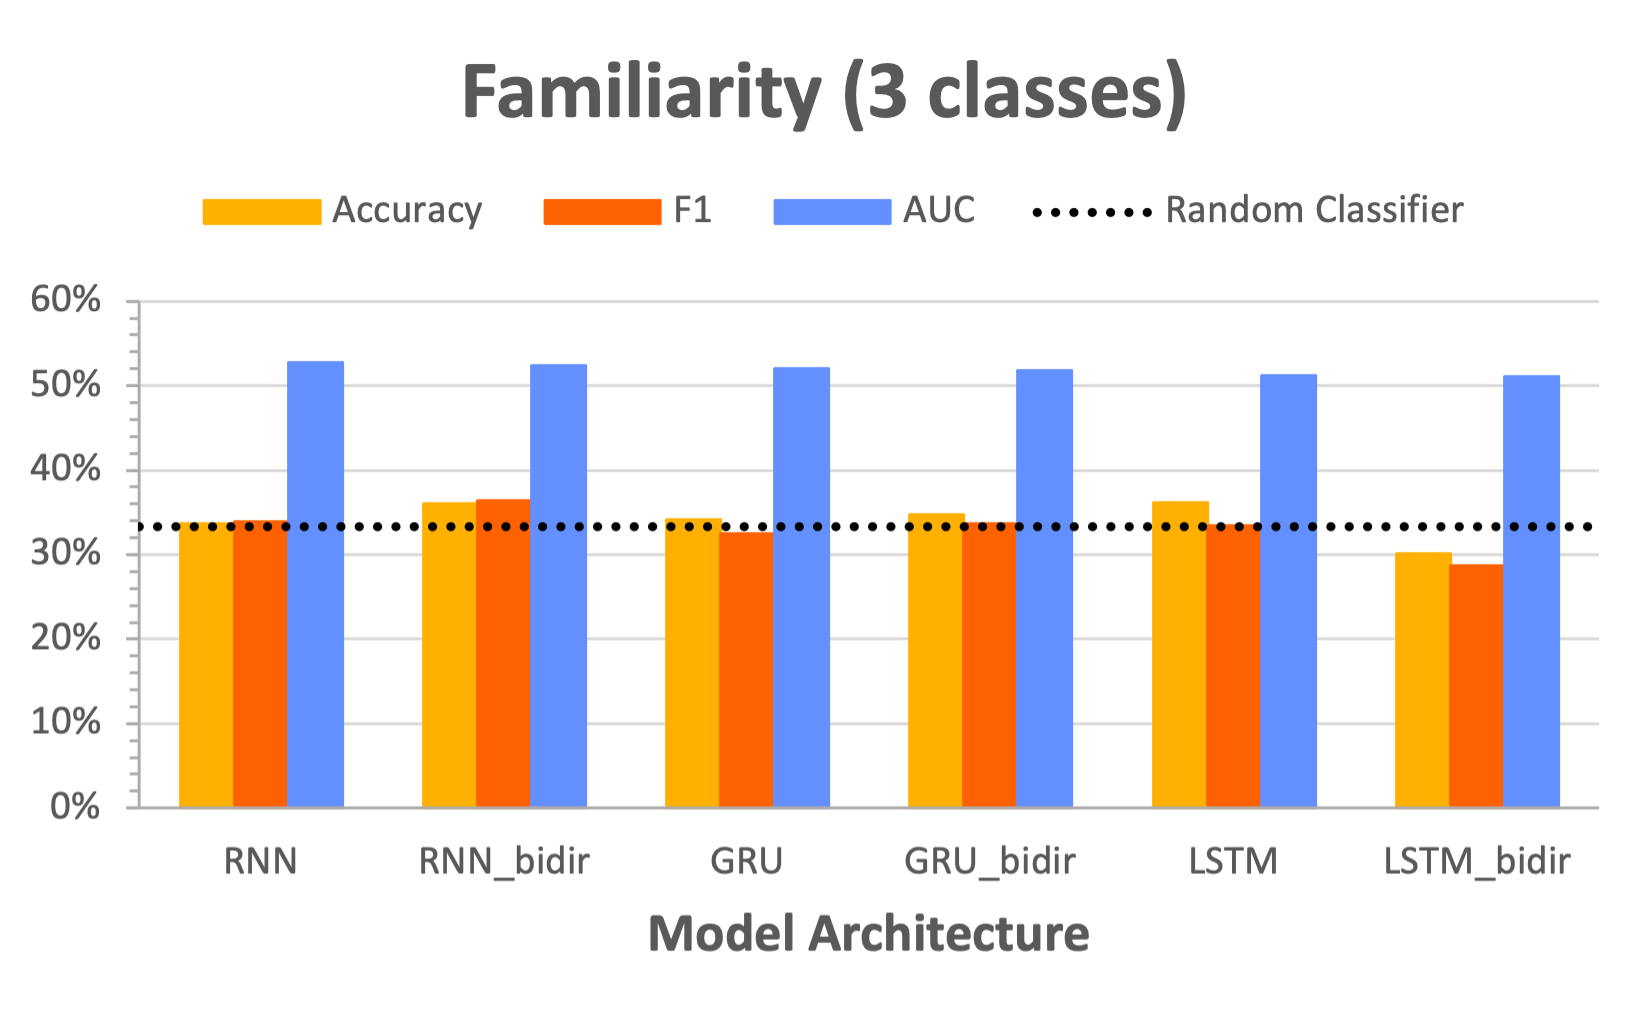
\includegraphics[width=\textwidth]{plots/model_fam.png}
         \caption{Layer type}
         \label{fig:models_fam}
     \end{subfigure}
     \hfill
     \begin{subfigure}{\w}
         \centering
         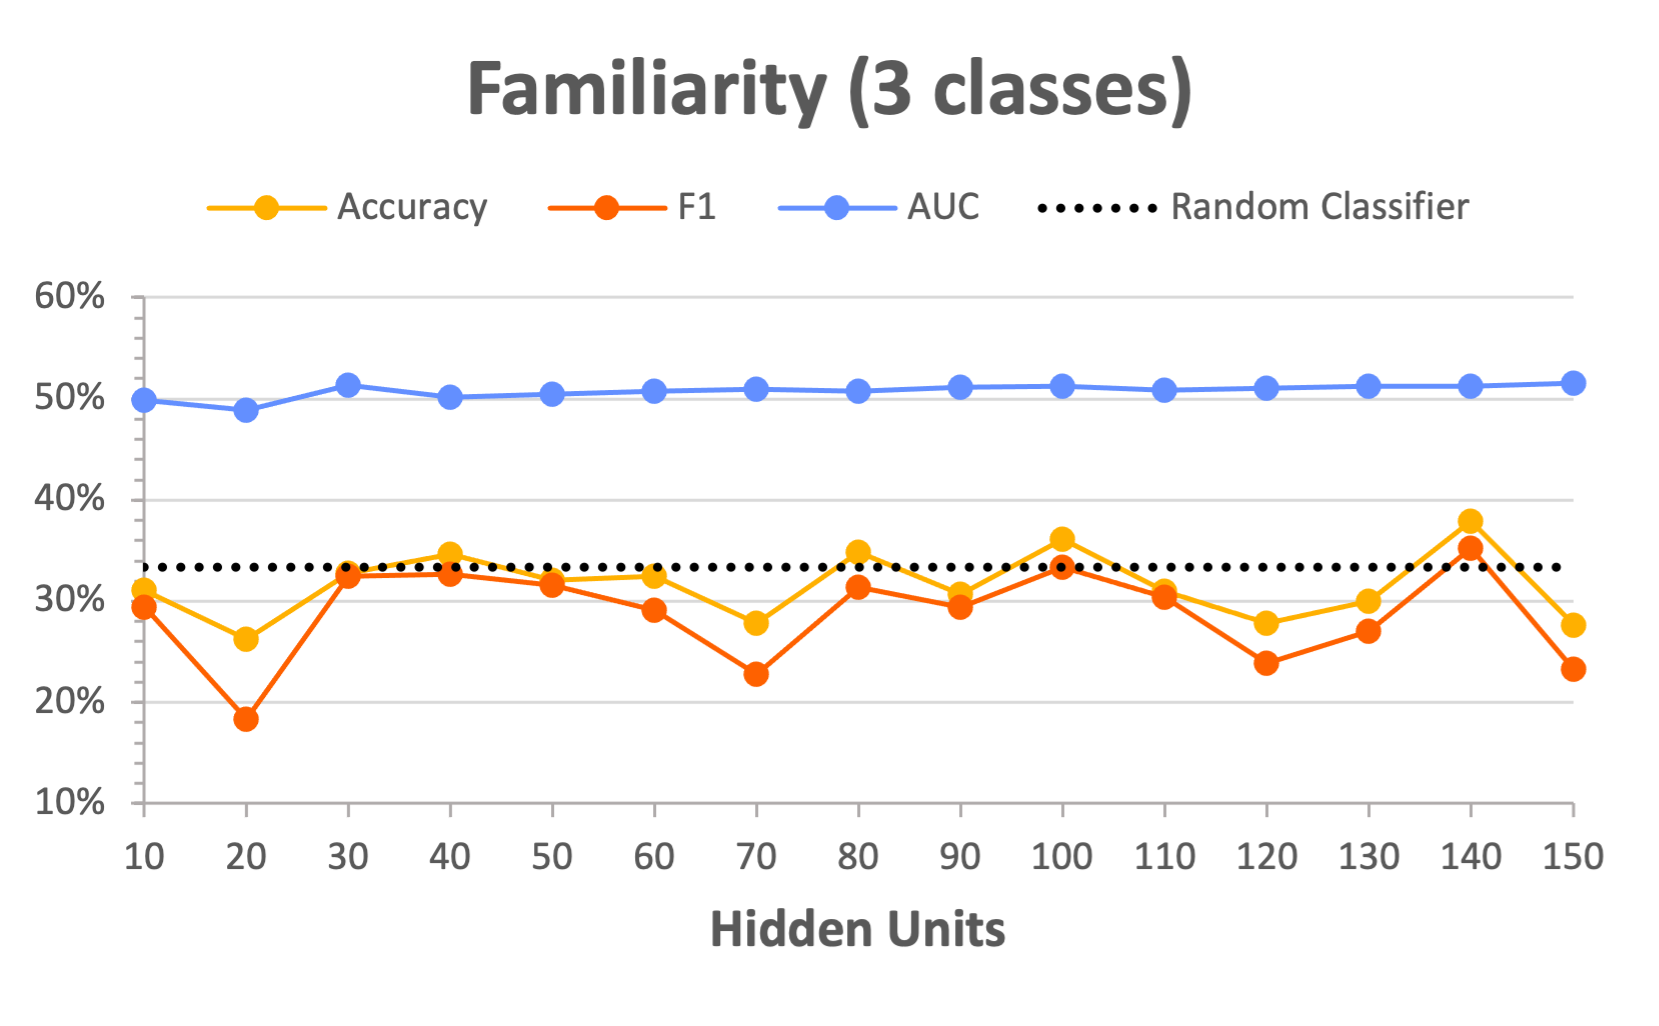
\includegraphics[width=\textwidth]{plots/units_fam.png}
         \caption{Hidden Units}
         \label{fig:units_fam}
     \end{subfigure}\\
     \begin{subfigure}{\w}
         \centering
         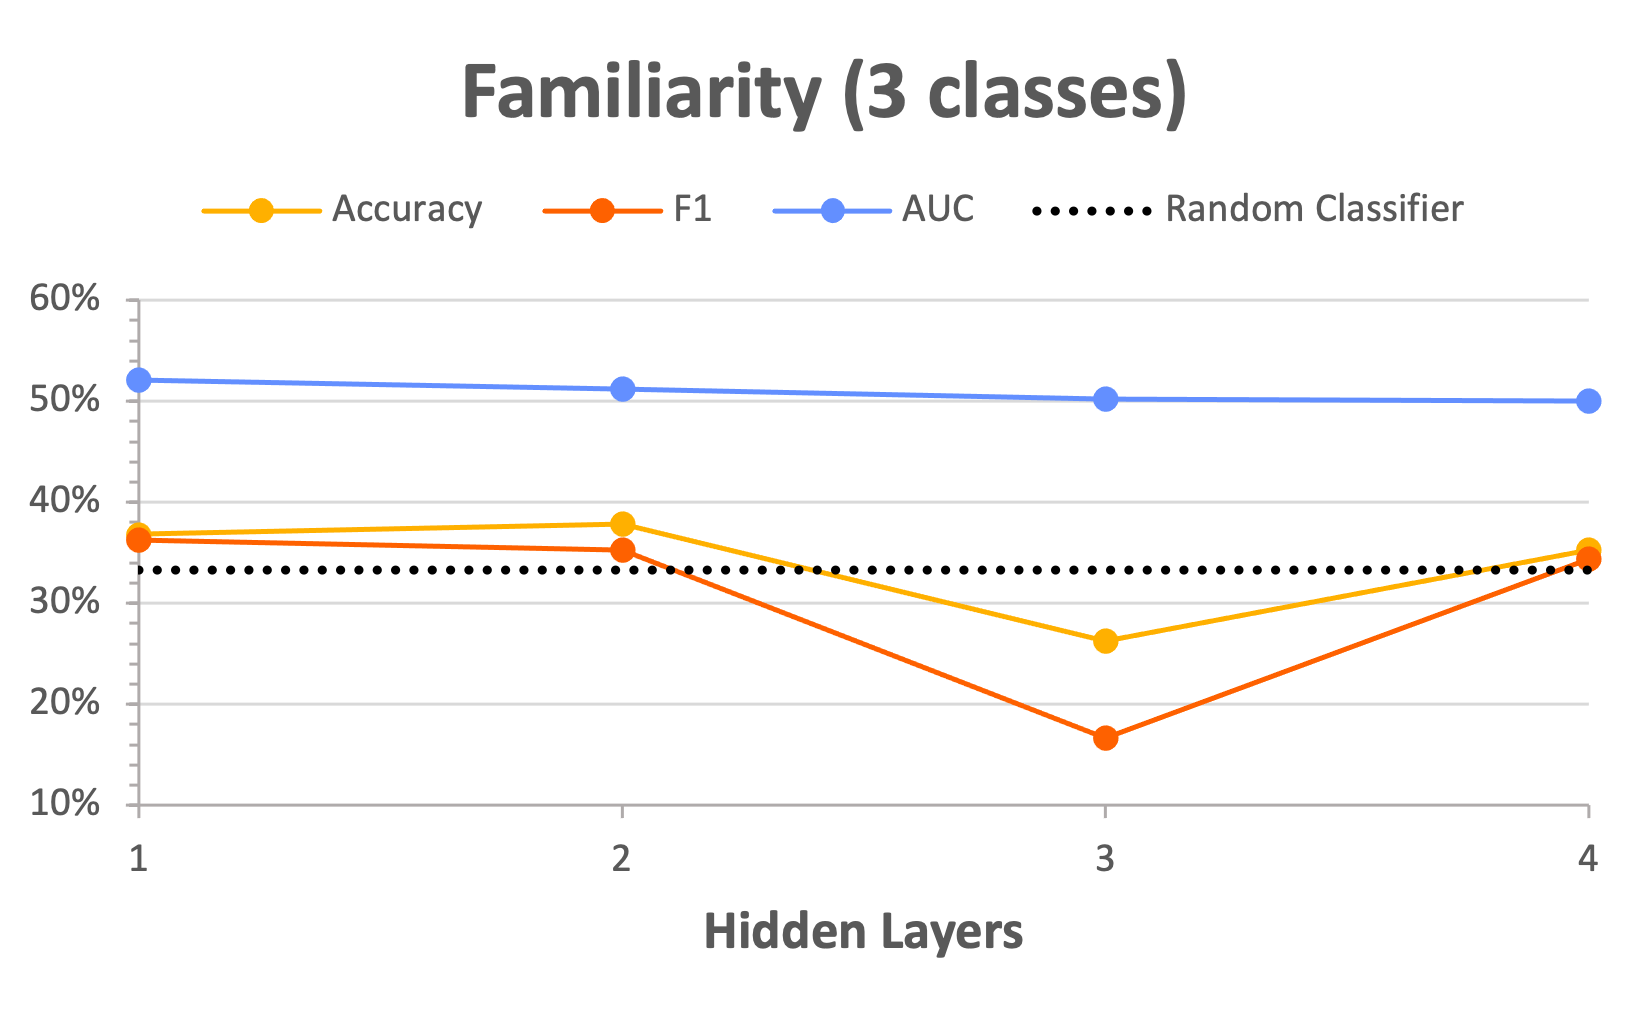
\includegraphics[width=\textwidth]{plots/layers_fam.png}
         \caption{Hidden Layers}
         \label{fig:layers_fam}
     \end{subfigure}
     \hfill
     \begin{subfigure}{\w}
         \centering
         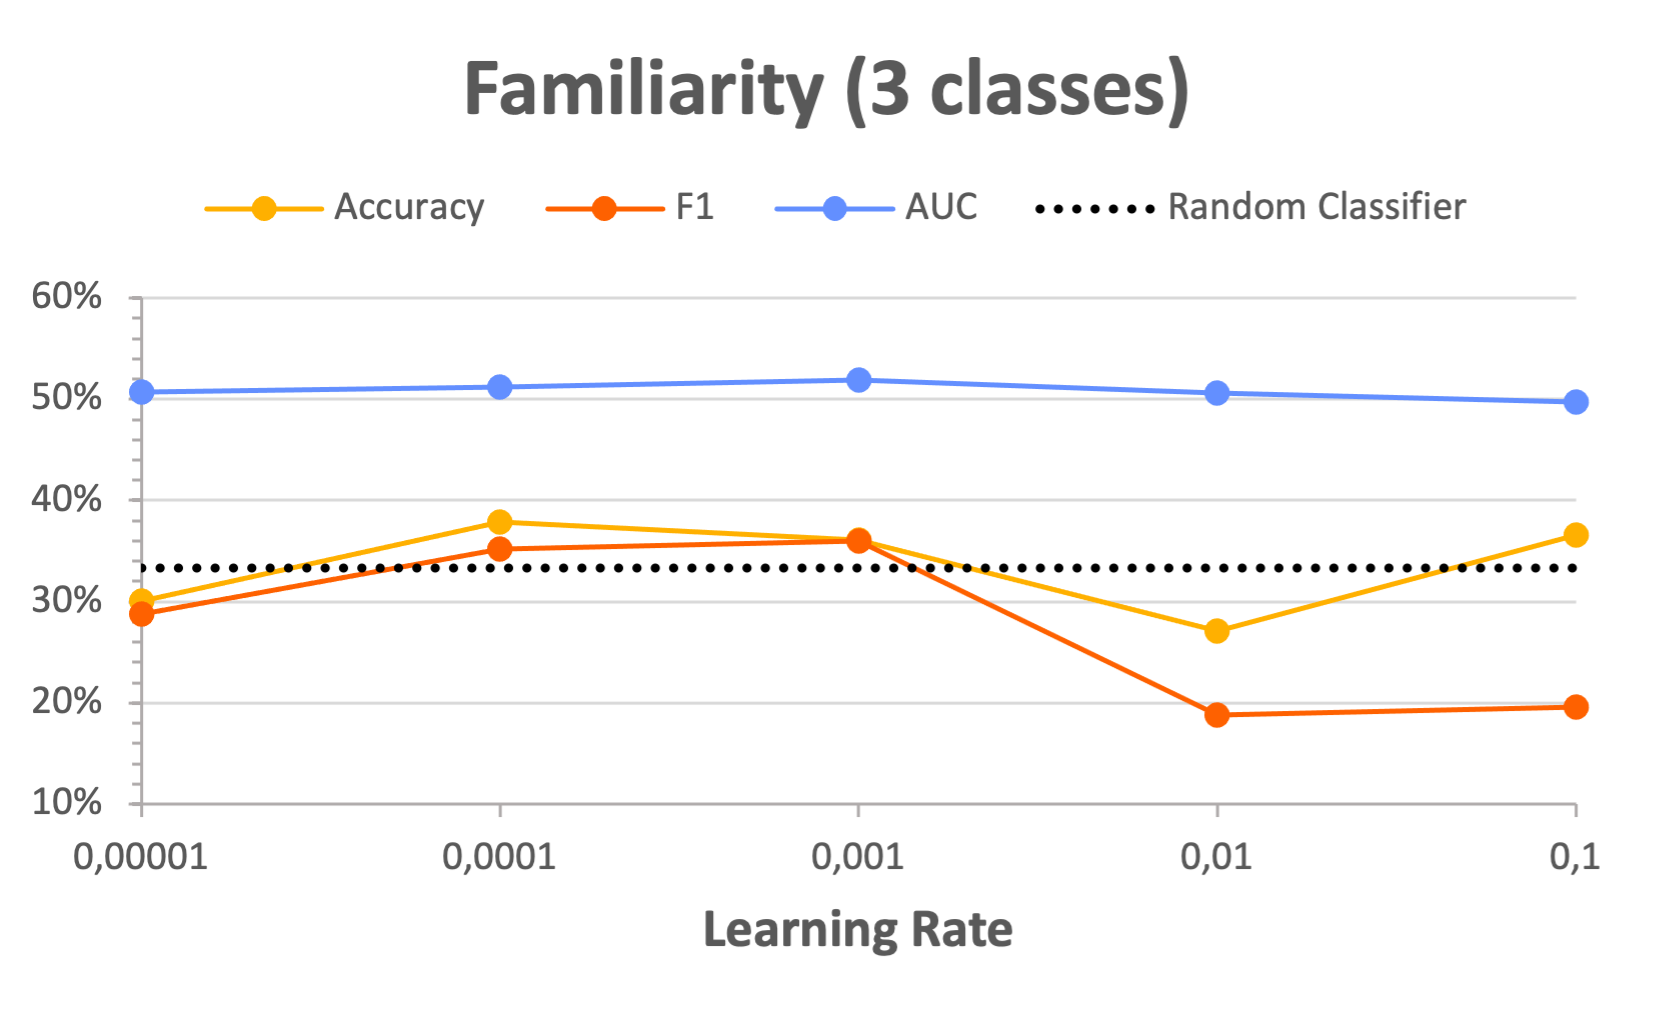
\includegraphics[width=\textwidth]{plots/lr_fam.png}
         \caption{Learning Rate}
         \label{fig:lr_fam}
     \end{subfigure}

    \caption{Predicting the user's swiping familiarity from swiped words trajectories.}
    \label{fig:fam}
\end{figure}

% For the swiping familiarity target \autoref{fig:fam}, with 3 classes, a random classifier's accuracy is 33,33\%.  The best performance accuracy achieved in our experiments is 37,87\%  with a the configuration: LSTM, 2 hidden layers, 140 hidden units and a learning rate of 10$^{-4}$.

\begin{figure}[]
     \centering
     \def\w{0.45\linewidth}
     \begin{subfigure}{\w}
         \centering
         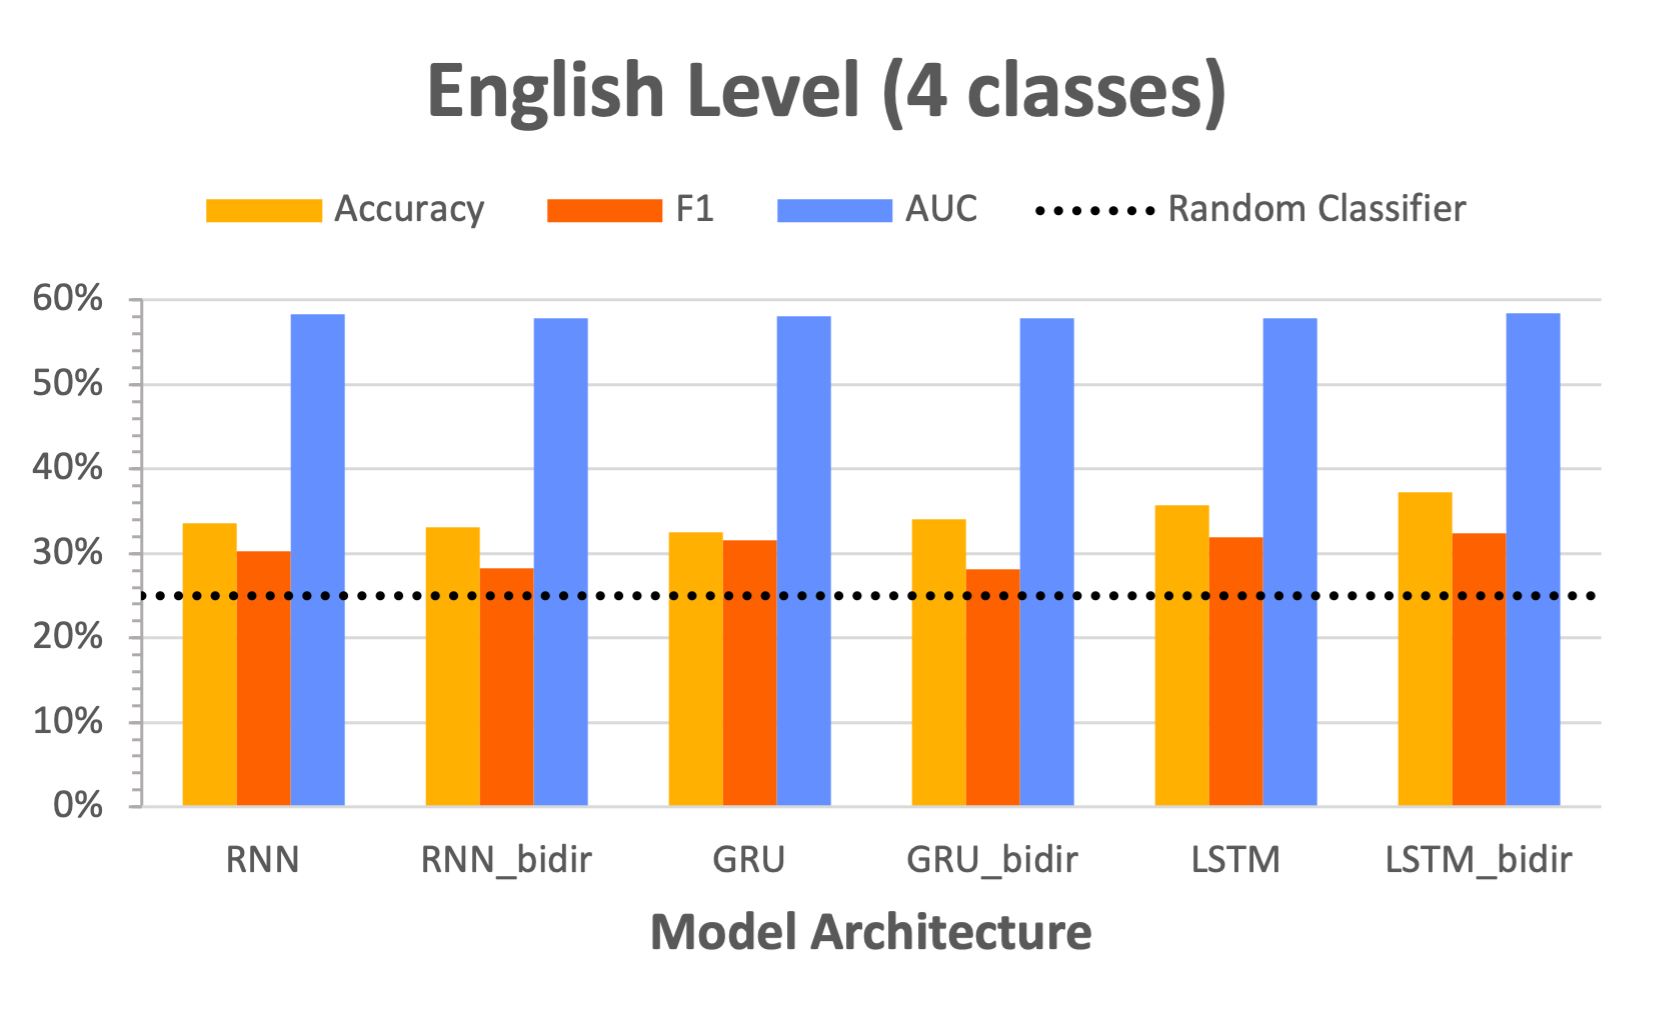
\includegraphics[width=\textwidth]{plots/model_english.png}
         \caption{Layer type}
         \label{fig:models_english}
     \end{subfigure}
     \hfill
     \begin{subfigure}{\w}
         \centering
         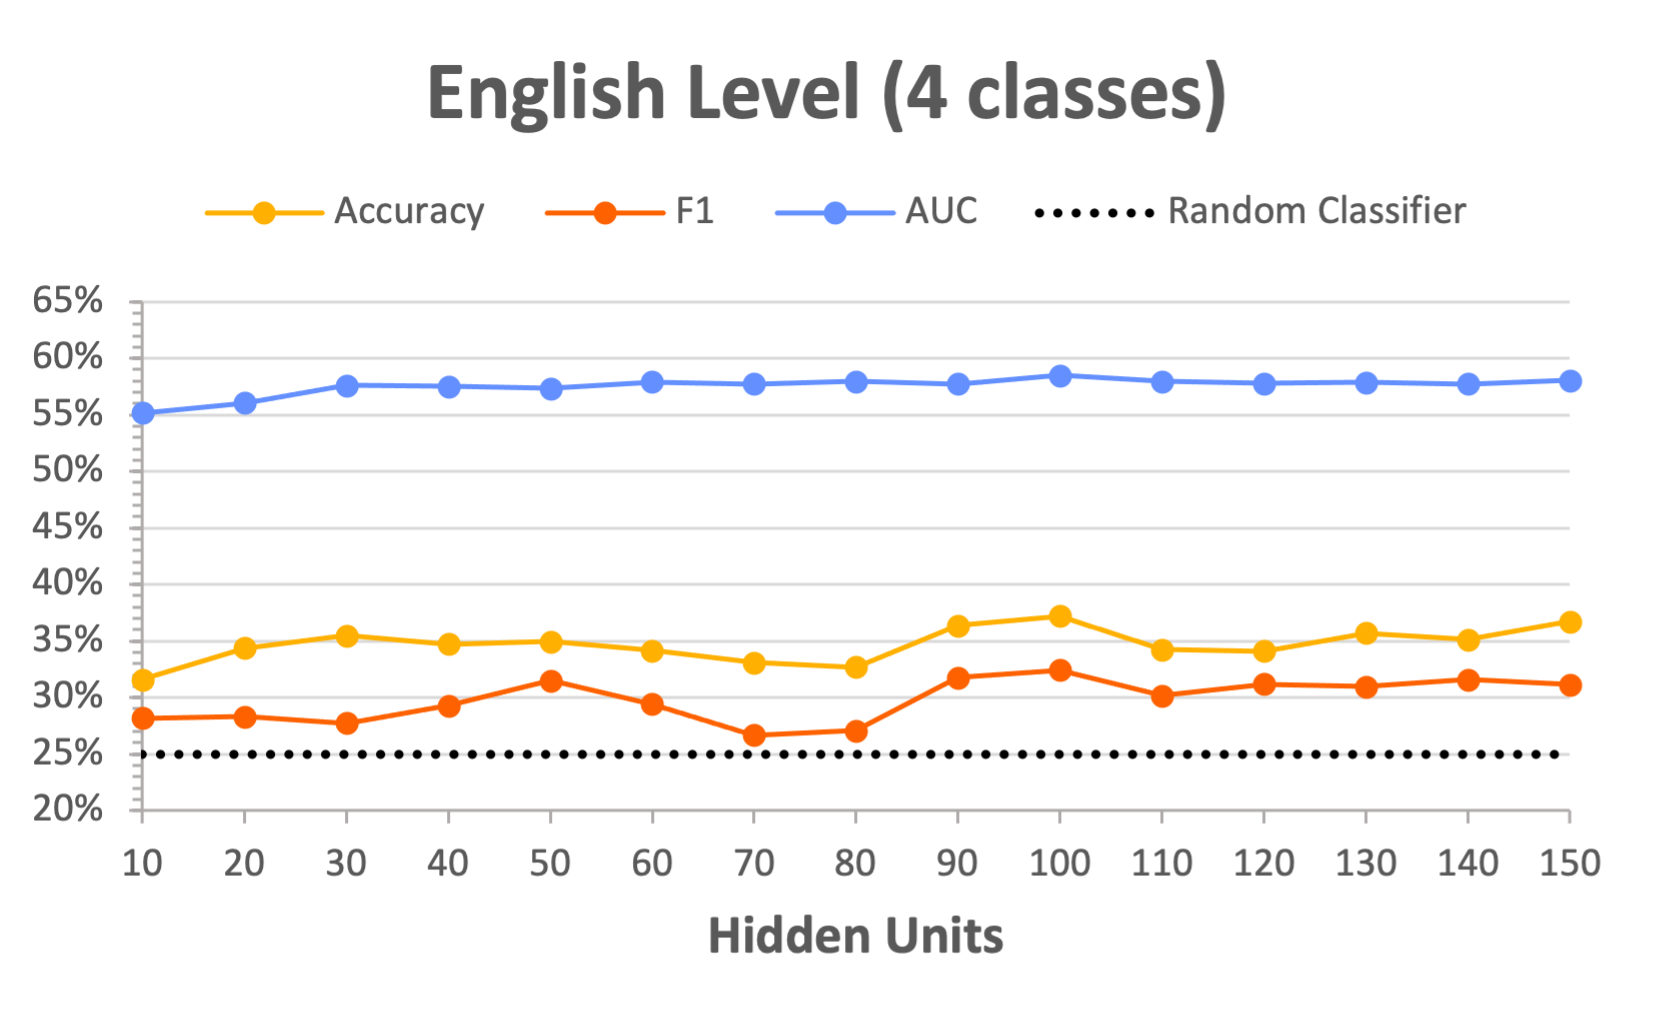
\includegraphics[width=\textwidth]{plots/units_english.png}
         \caption{Hidden Units}
         \label{fig:units_english}
     \end{subfigure}\\
     \begin{subfigure}{\w}
         \centering
         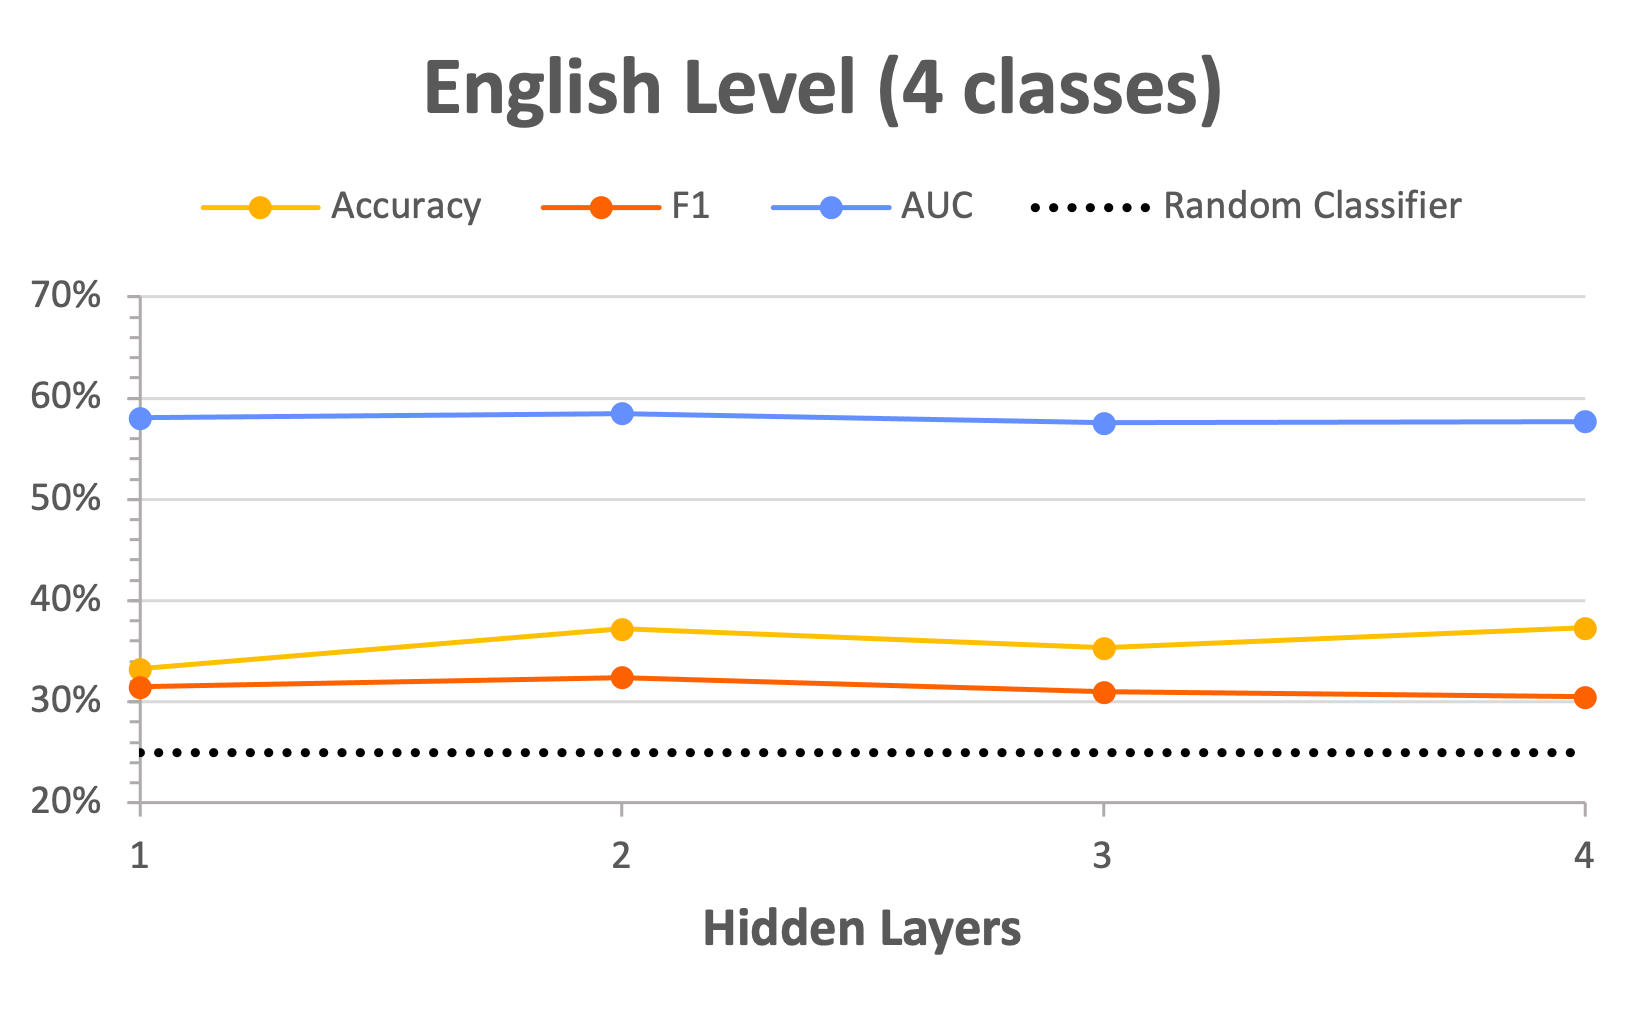
\includegraphics[width=\textwidth]{plots/layers_english.png}
         \caption{Hidden Layers}
         \label{fig:layers_english}
     \end{subfigure}
     \hfill
     \begin{subfigure}{\w}
         \centering
         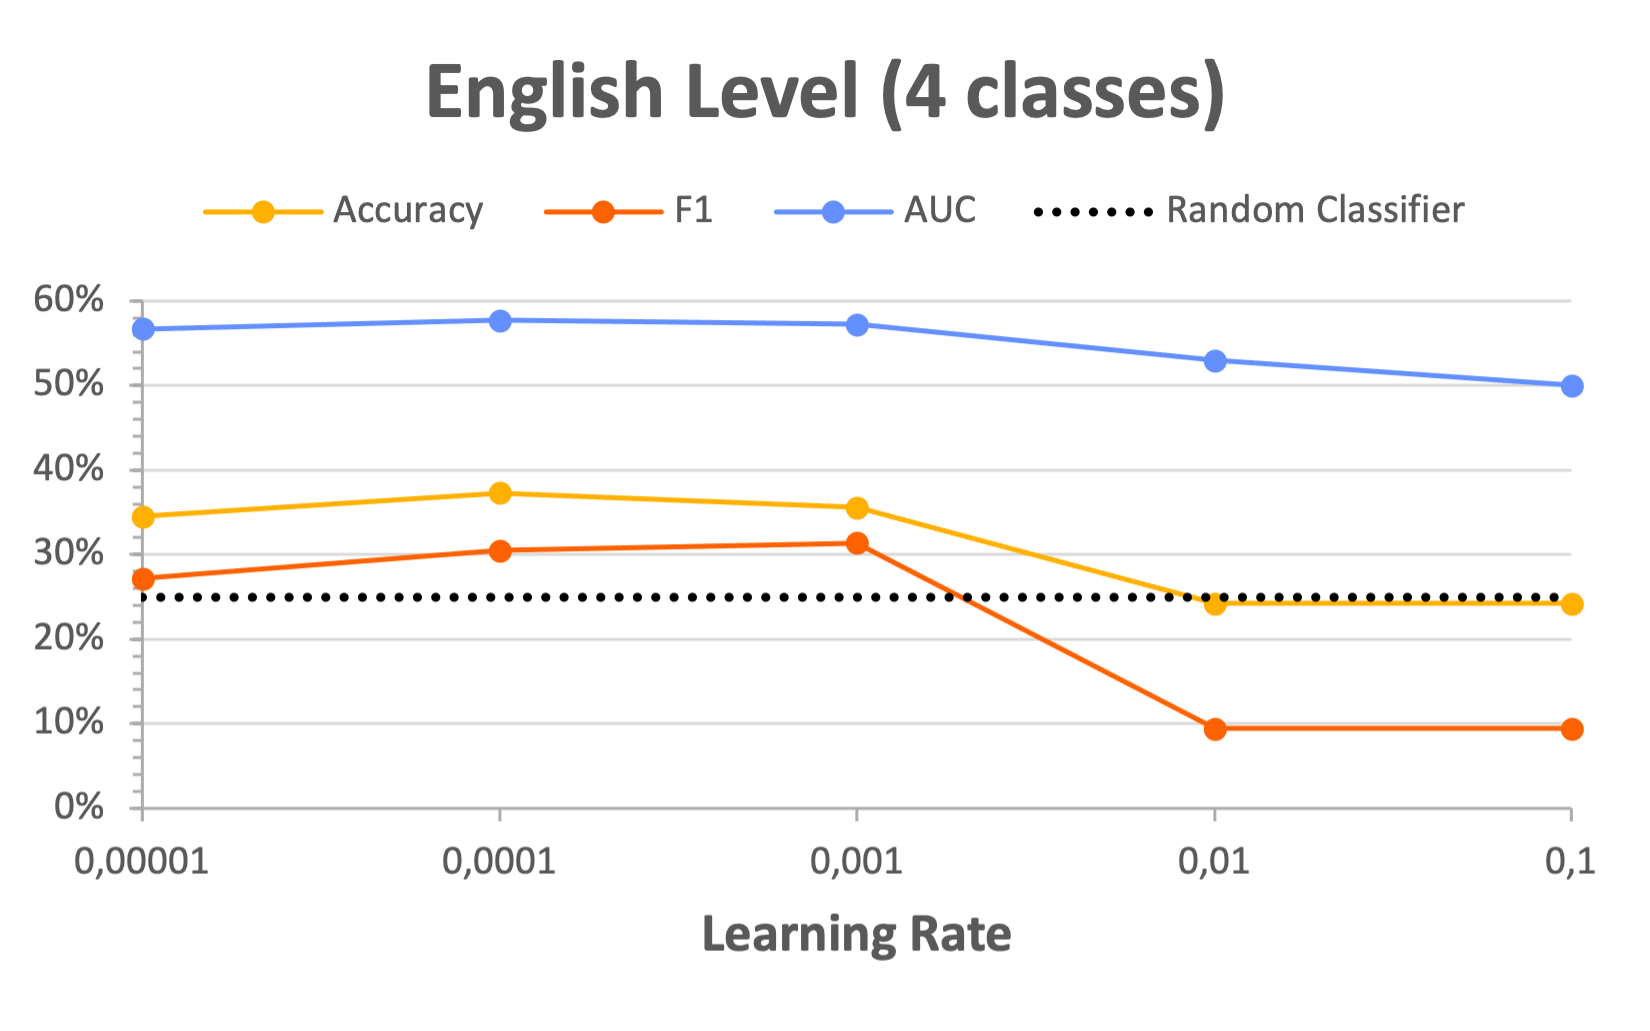
\includegraphics[width=\textwidth]{plots/lr_english.png}
         \caption{Learning Rate}
         \label{fig:lr_english}
     \end{subfigure}

    \caption{Predicting the user's English level from swiped words trajectories.}
    \label{fig:engl}
\end{figure}

% For the English level target \autoref{fig:engl}, with 4 classes, a random classifier's accuracy is 25\%. The best performance accuracy achieved in our experiments is 37,32\% with the configuration: BiLSTM , 4 hidden layers, 100 hidden units and a learning rate of 10$^{-4}$.

\begin{figure}[]
     \centering
     \def\w{0.45\linewidth}
     \begin{subfigure}{\w}
         \centering
         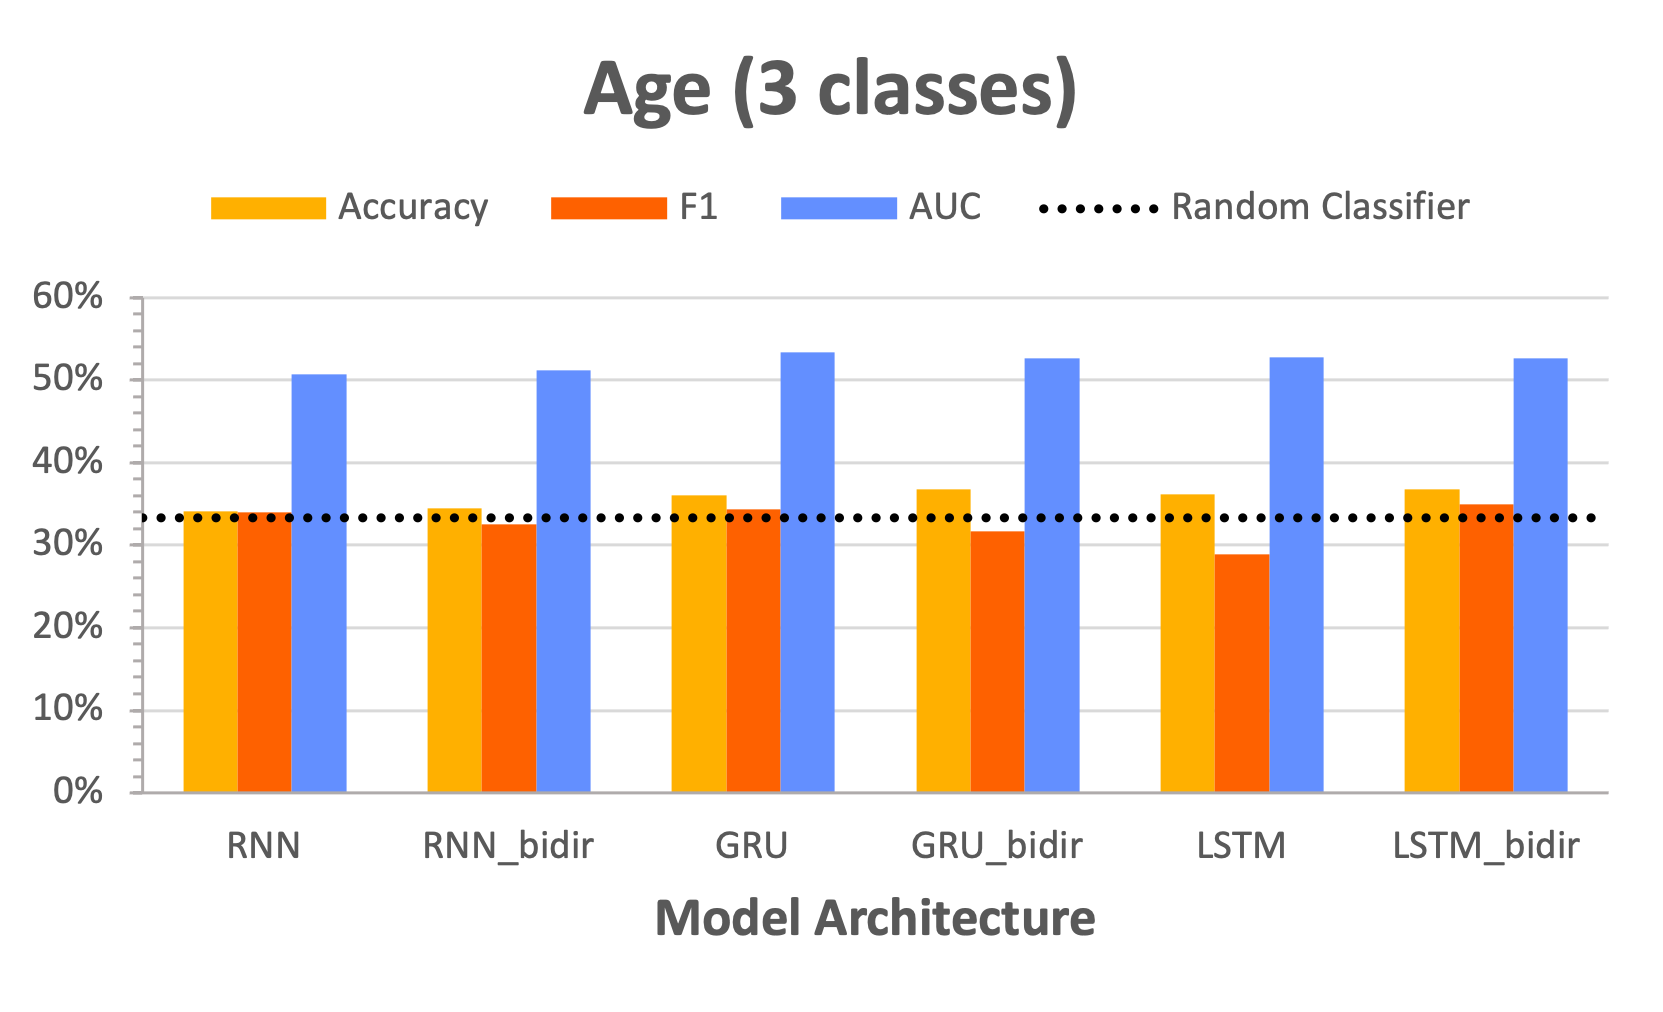
\includegraphics[width=\textwidth]{plots/model_age.png}
         \caption{Layer type}
         \label{fig:models_age}
     \end{subfigure}
     \hfill
     \begin{subfigure}{\w}
         \centering
         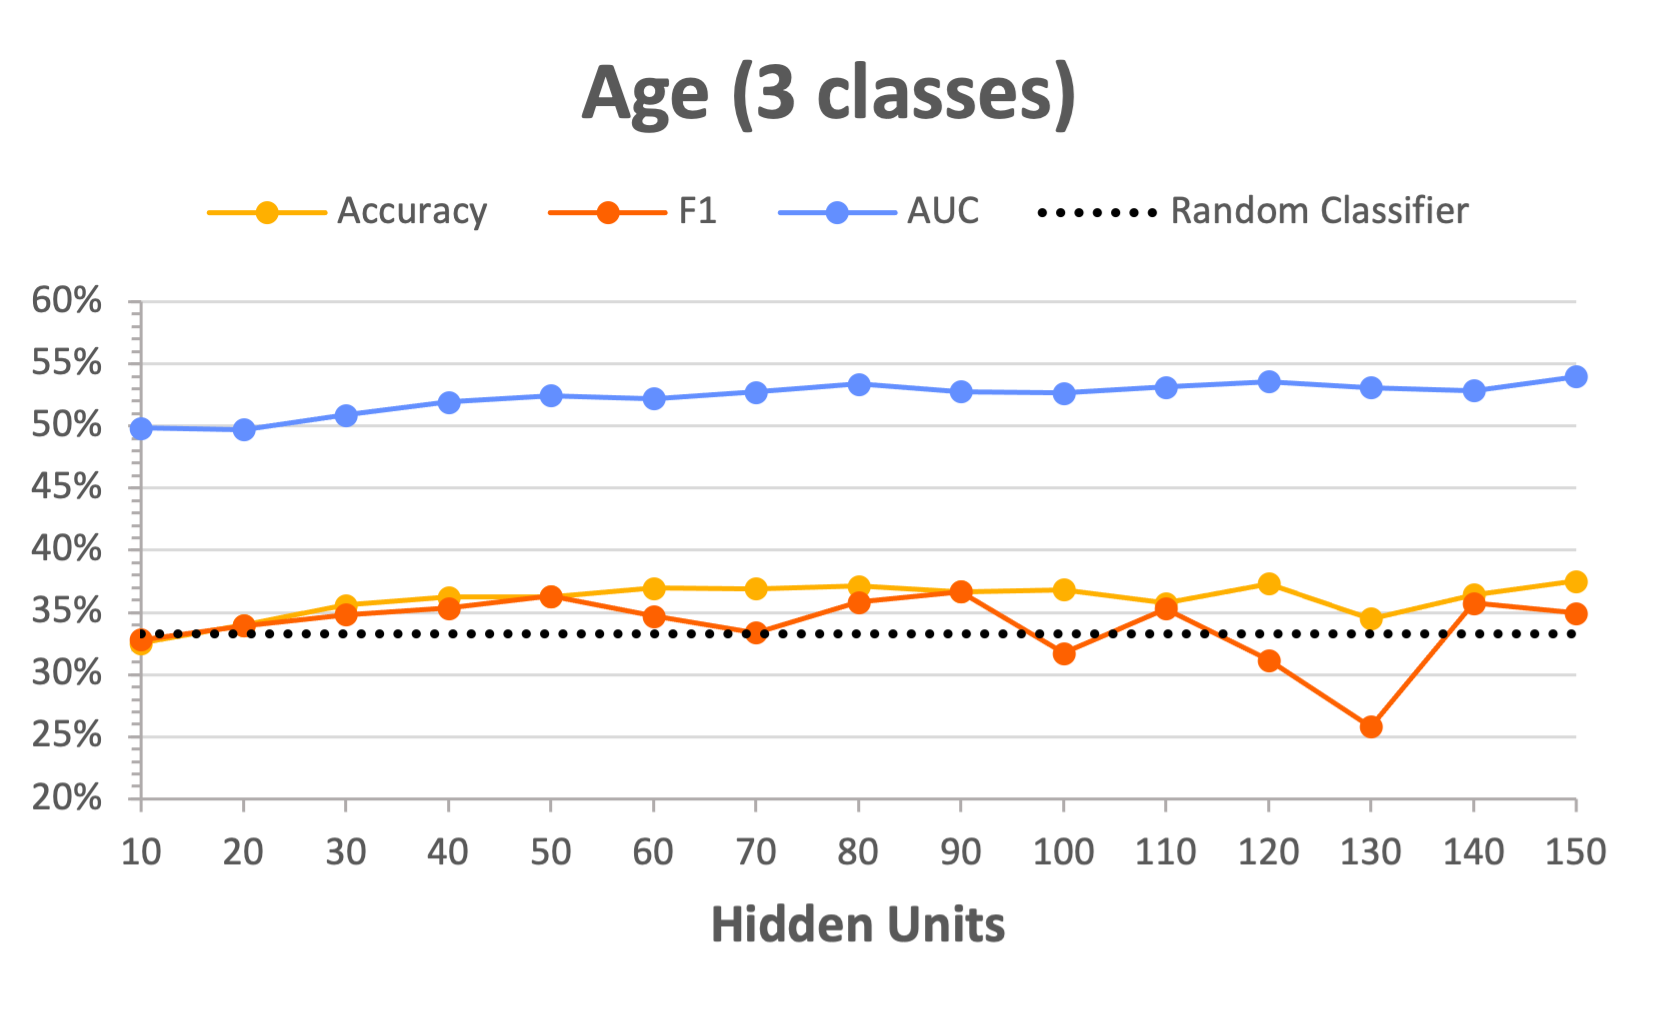
\includegraphics[width=\textwidth]{plots/units_age.png}
         \caption{Hidden Units}
         \label{fig:units_age}
     \end{subfigure}\\
     \begin{subfigure}{\w}
         \centering
         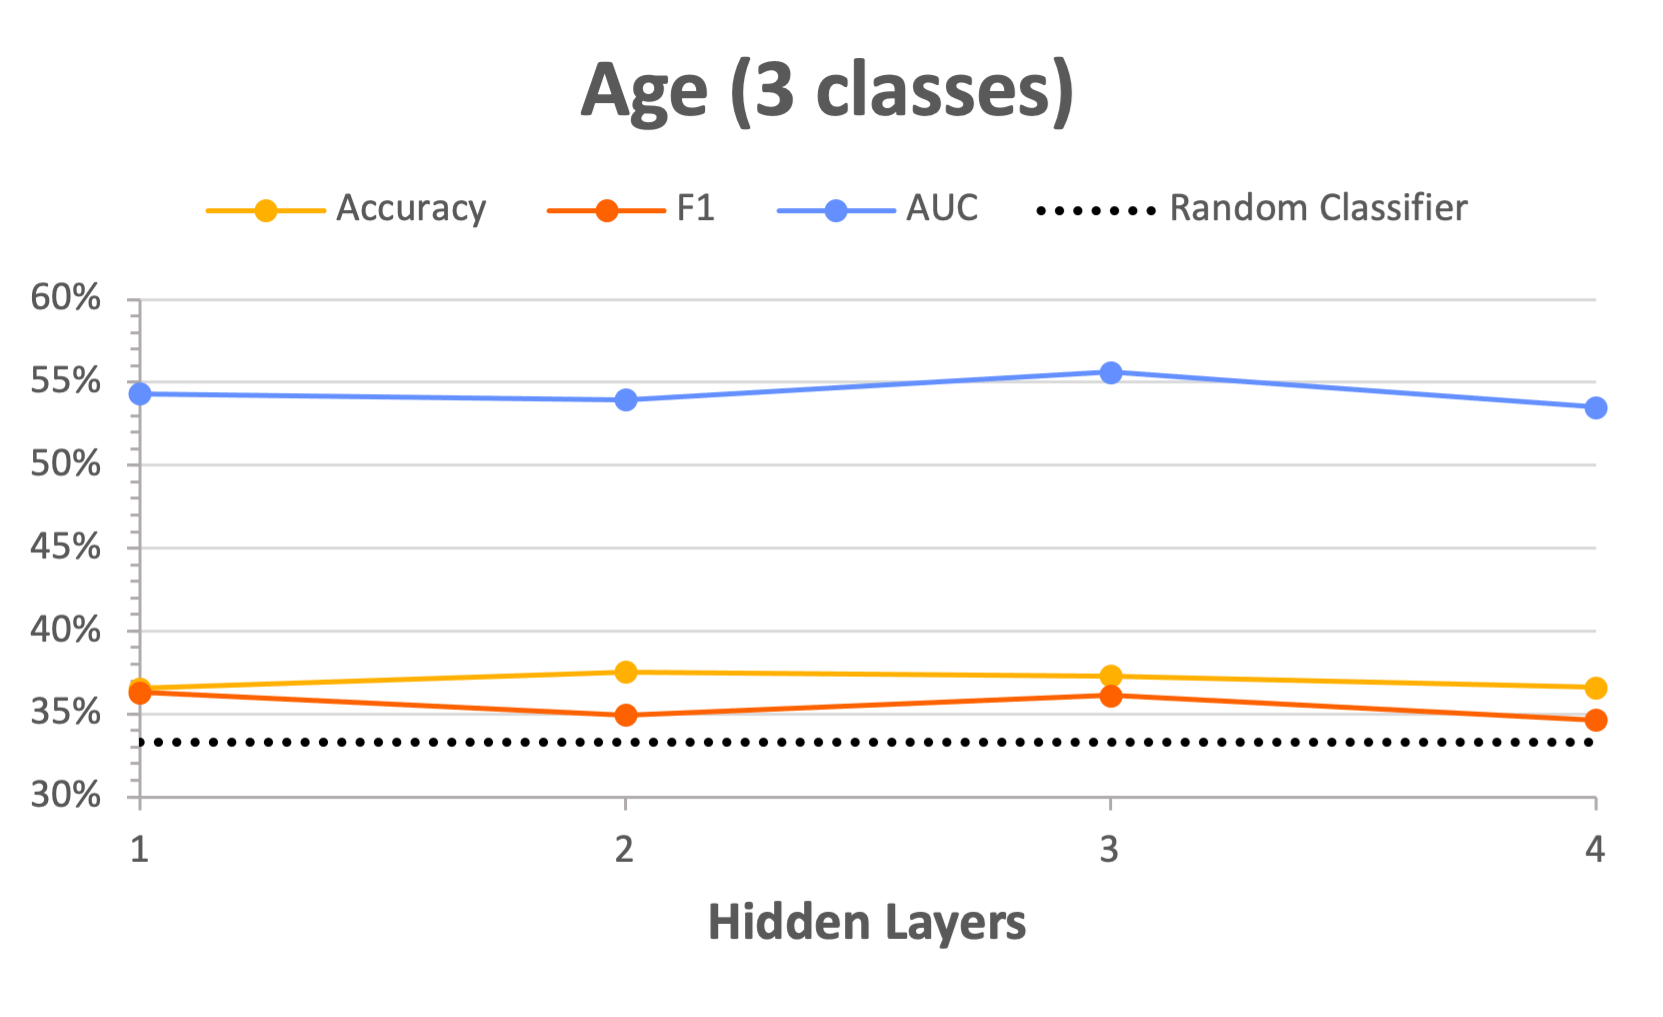
\includegraphics[width=\textwidth]{plots/layers_age.png}
         \caption{Hidden Layers}
         \label{fig:layers_age}
     \end{subfigure}
     \hfill
     \begin{subfigure}{\w}
         \centering
         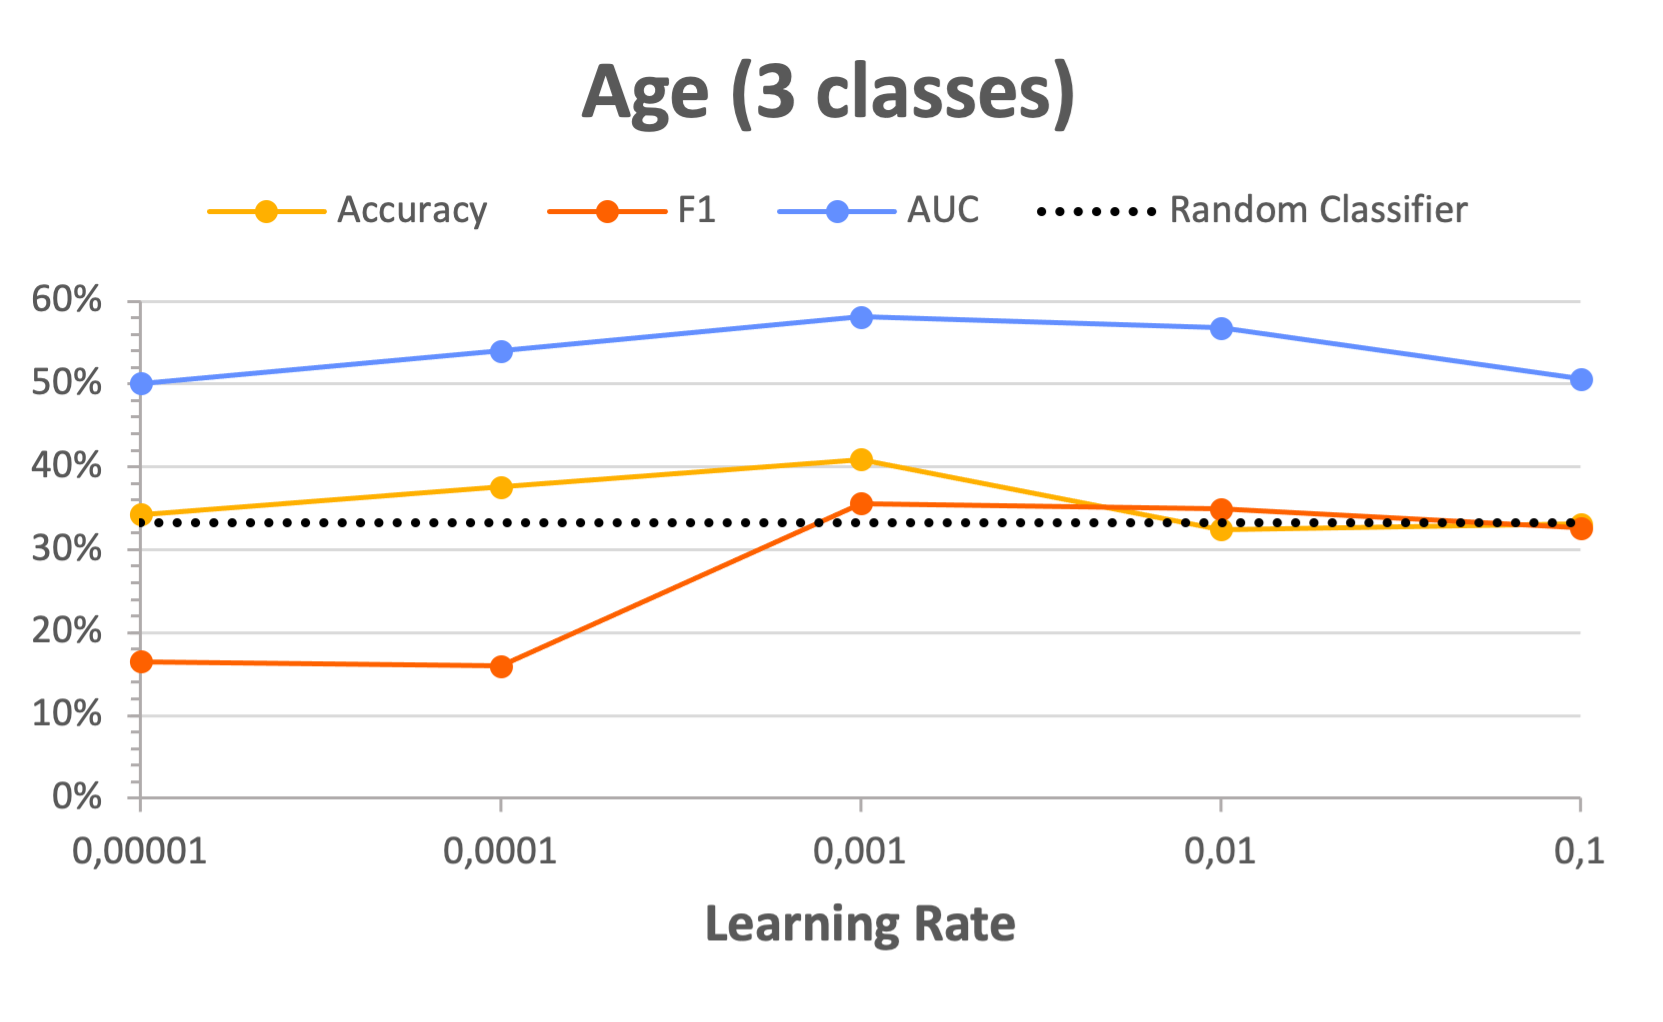
\includegraphics[width=\textwidth]{plots/lr_age.png}
         \caption{Learning Rate}
         \label{fig:lr_age}
     \end{subfigure}

    \caption{Predicting the user's age from swiped words trajectories.}
    \label{fig:age}
\end{figure}

% For the Age target \autoref{fig:age}, with 3 classes the accuracy of a random classifier is 33,33\% . Whereas,  the best performance accuracy achieved in our experiments is 40,91\% with the configuration: BiGRU, 2 hidden layers, 150 hidden units and a learning rate of 10$^{-3}$.

\begin{figure}[]
     \centering
     \def\w{0.4\linewidth}
     \begin{subfigure}{\w}
         \centering
         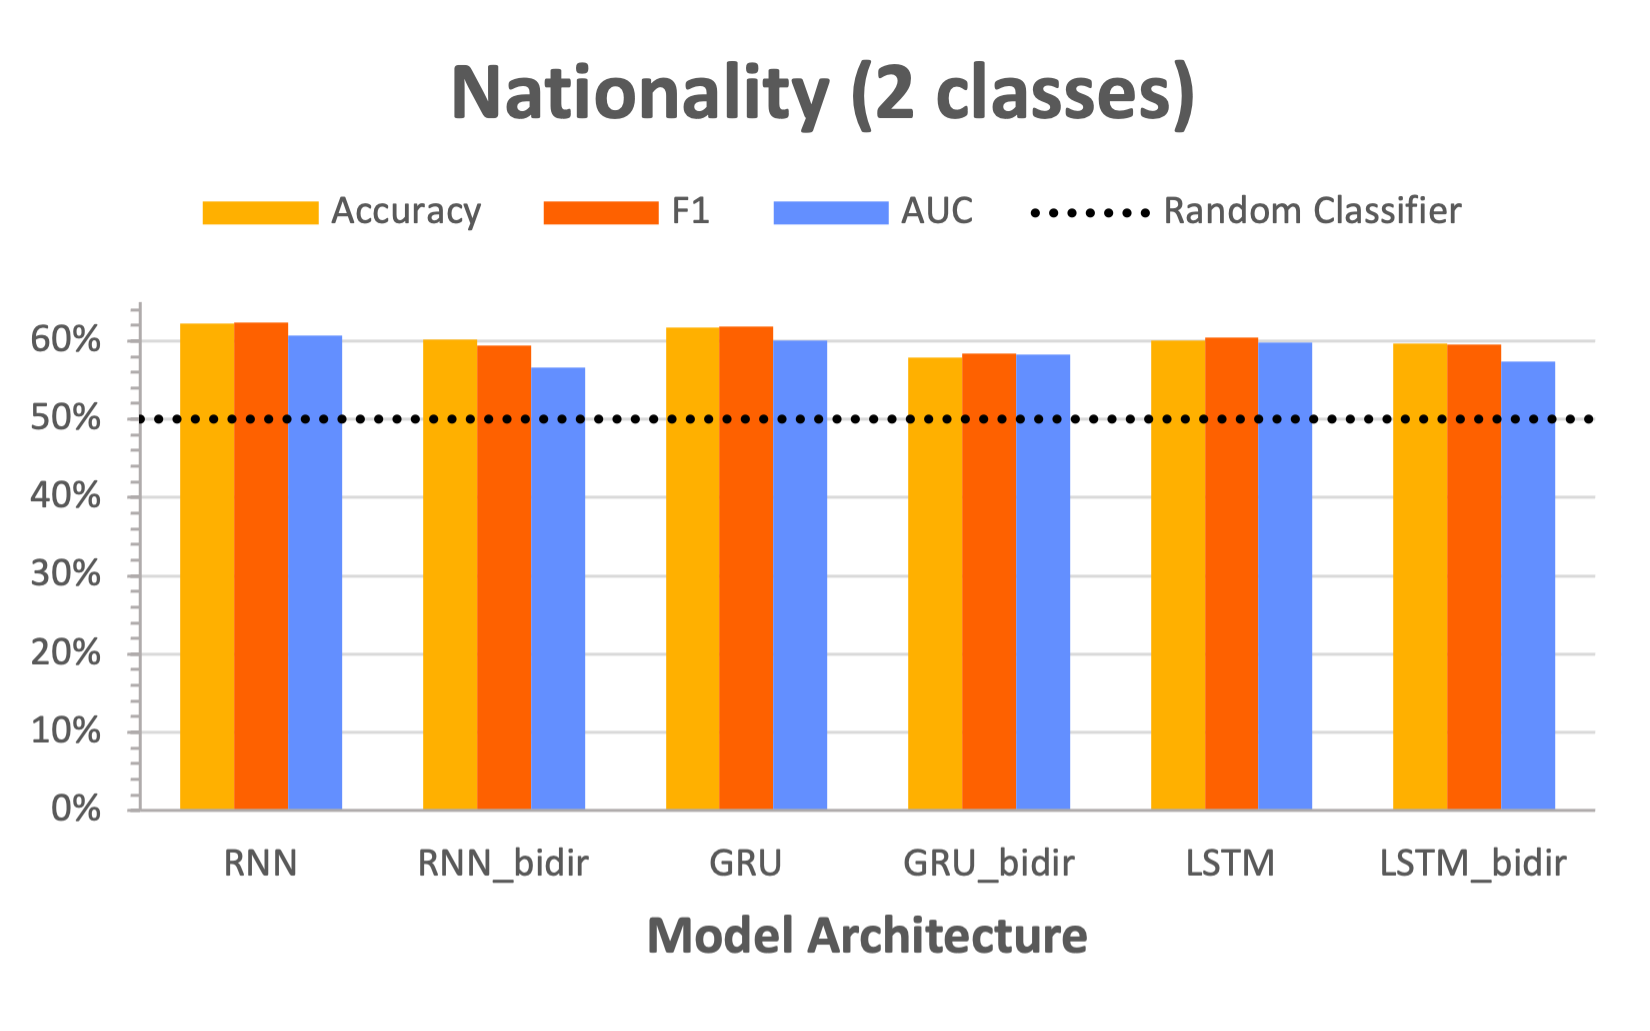
\includegraphics[width=\textwidth]{plots/model_nat.png}
         \caption{Layer type}
         \label{fig:models_nat}
     \end{subfigure}
     \hfill
     \begin{subfigure}{\w}
         \centering
         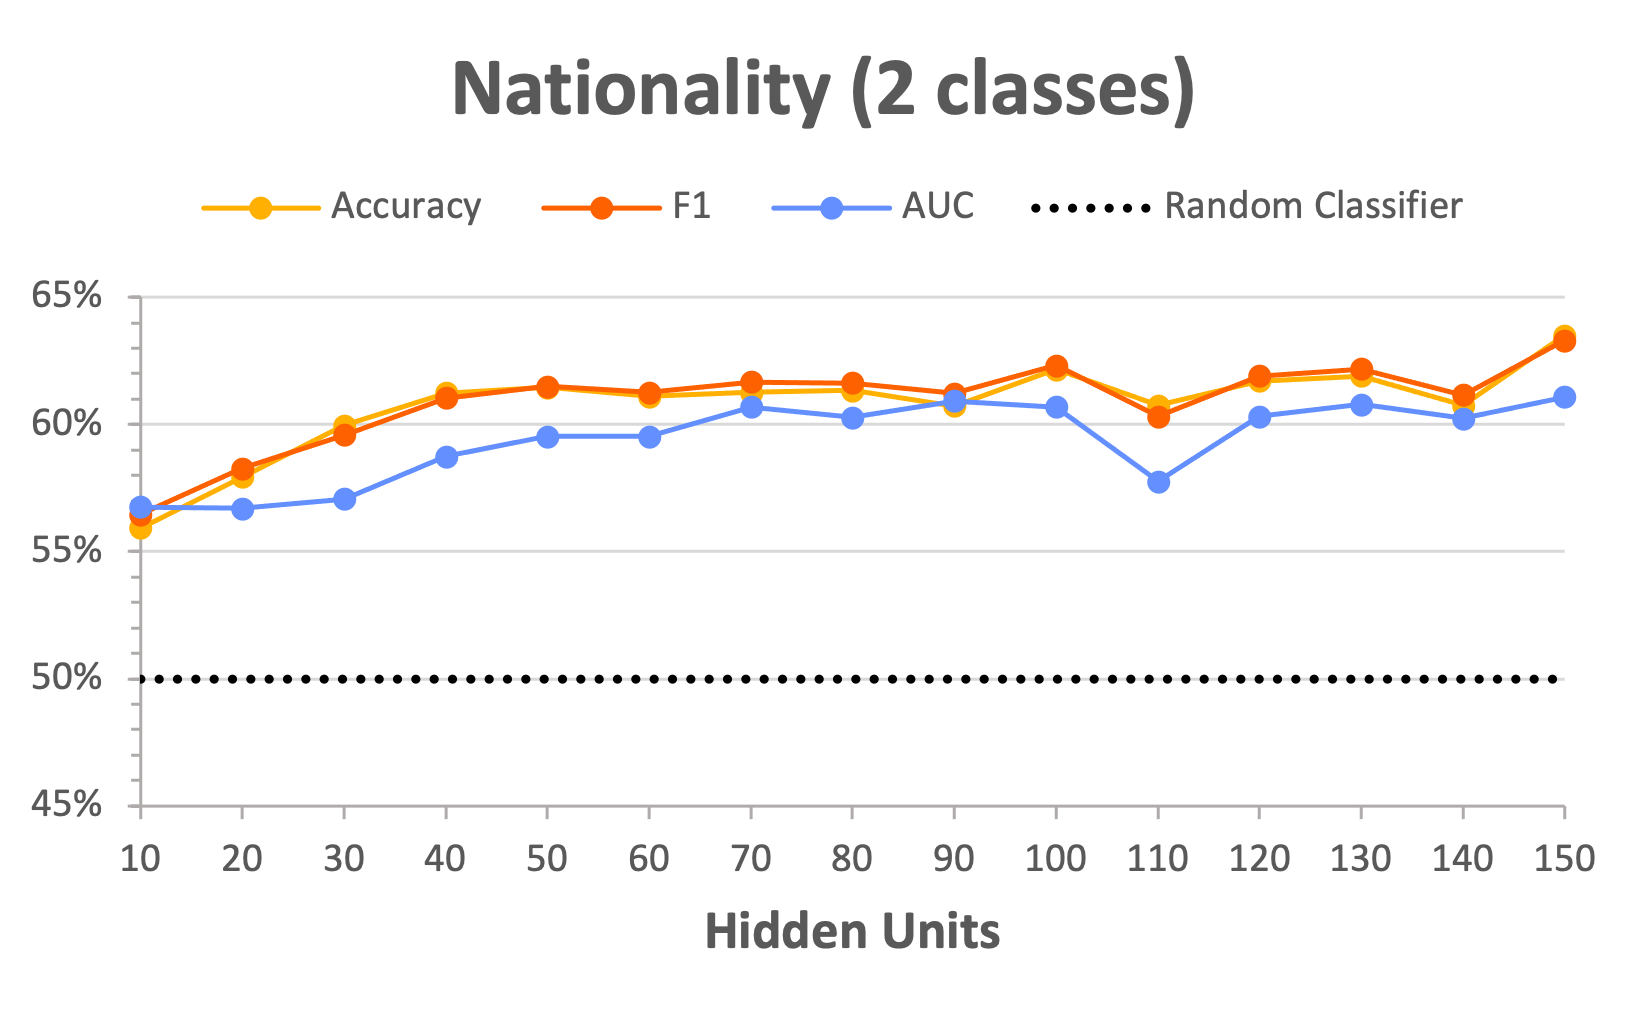
\includegraphics[width=\textwidth]{plots/units_nat.png}
         \caption{Hidden Units}
         \label{fig:units_nat}
     \end{subfigure}\\
     \begin{subfigure}{\w}
         \centering
         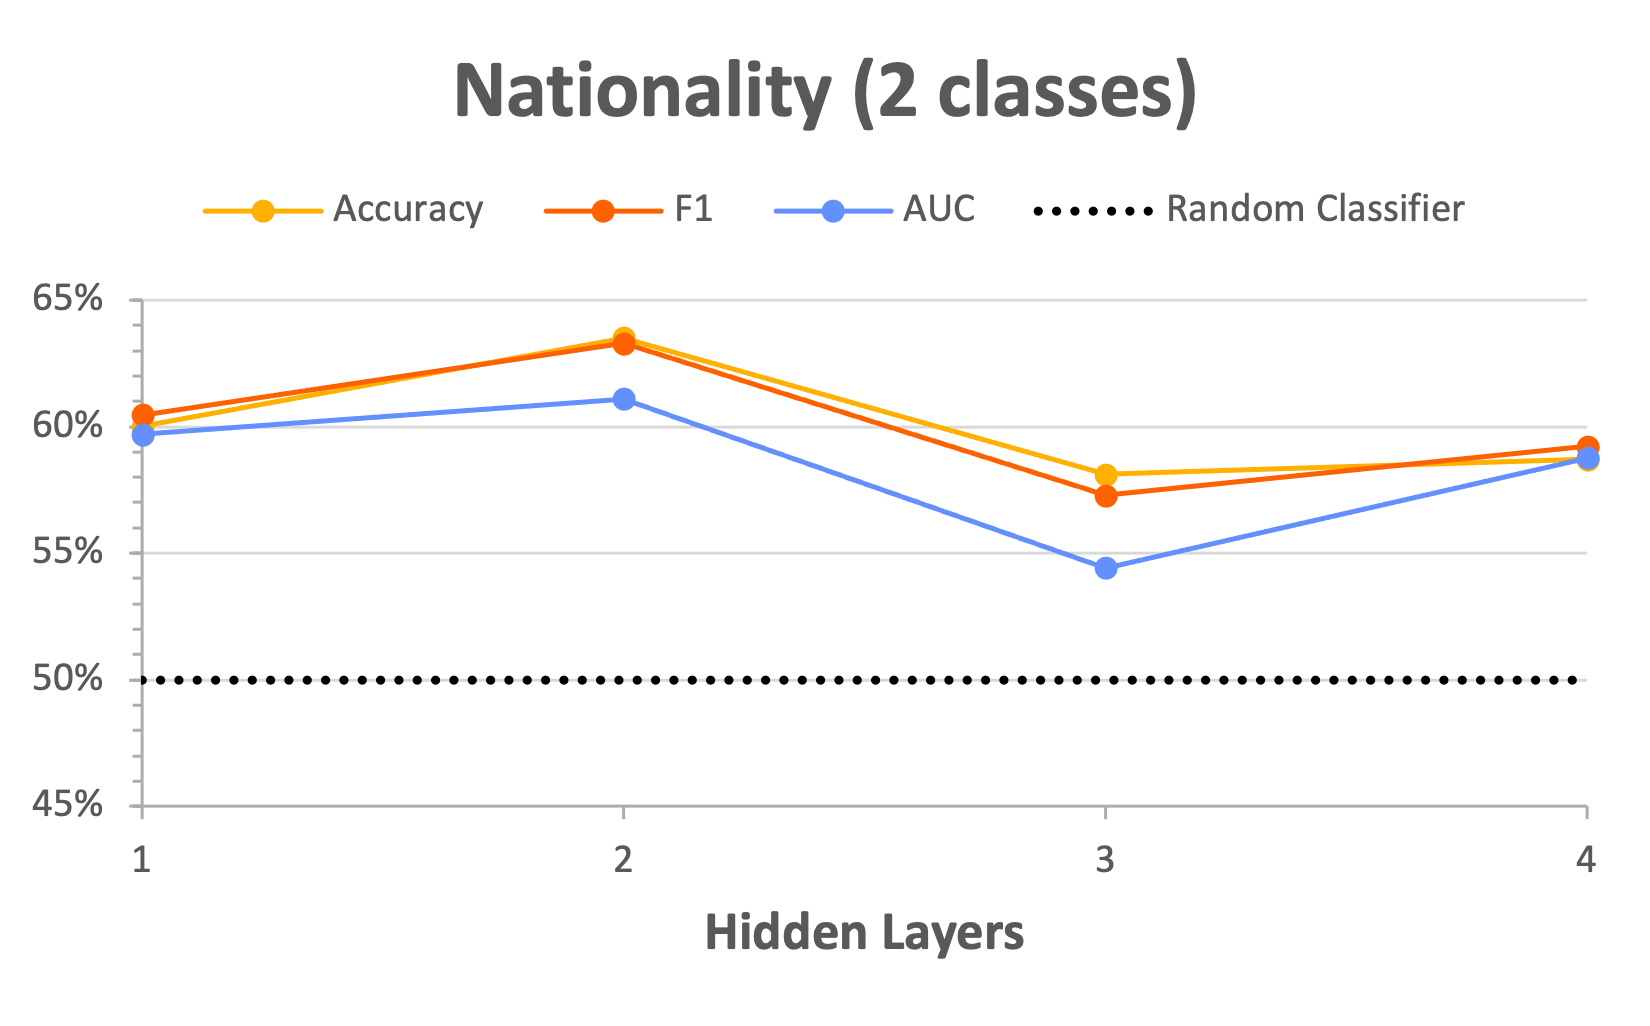
\includegraphics[width=\textwidth]{plots/layers_nat.png}
         \caption{Hidden Layers}
         \label{fig:layers_nat}
     \end{subfigure}
     \hfill
     \begin{subfigure}{\w}
         \centering
         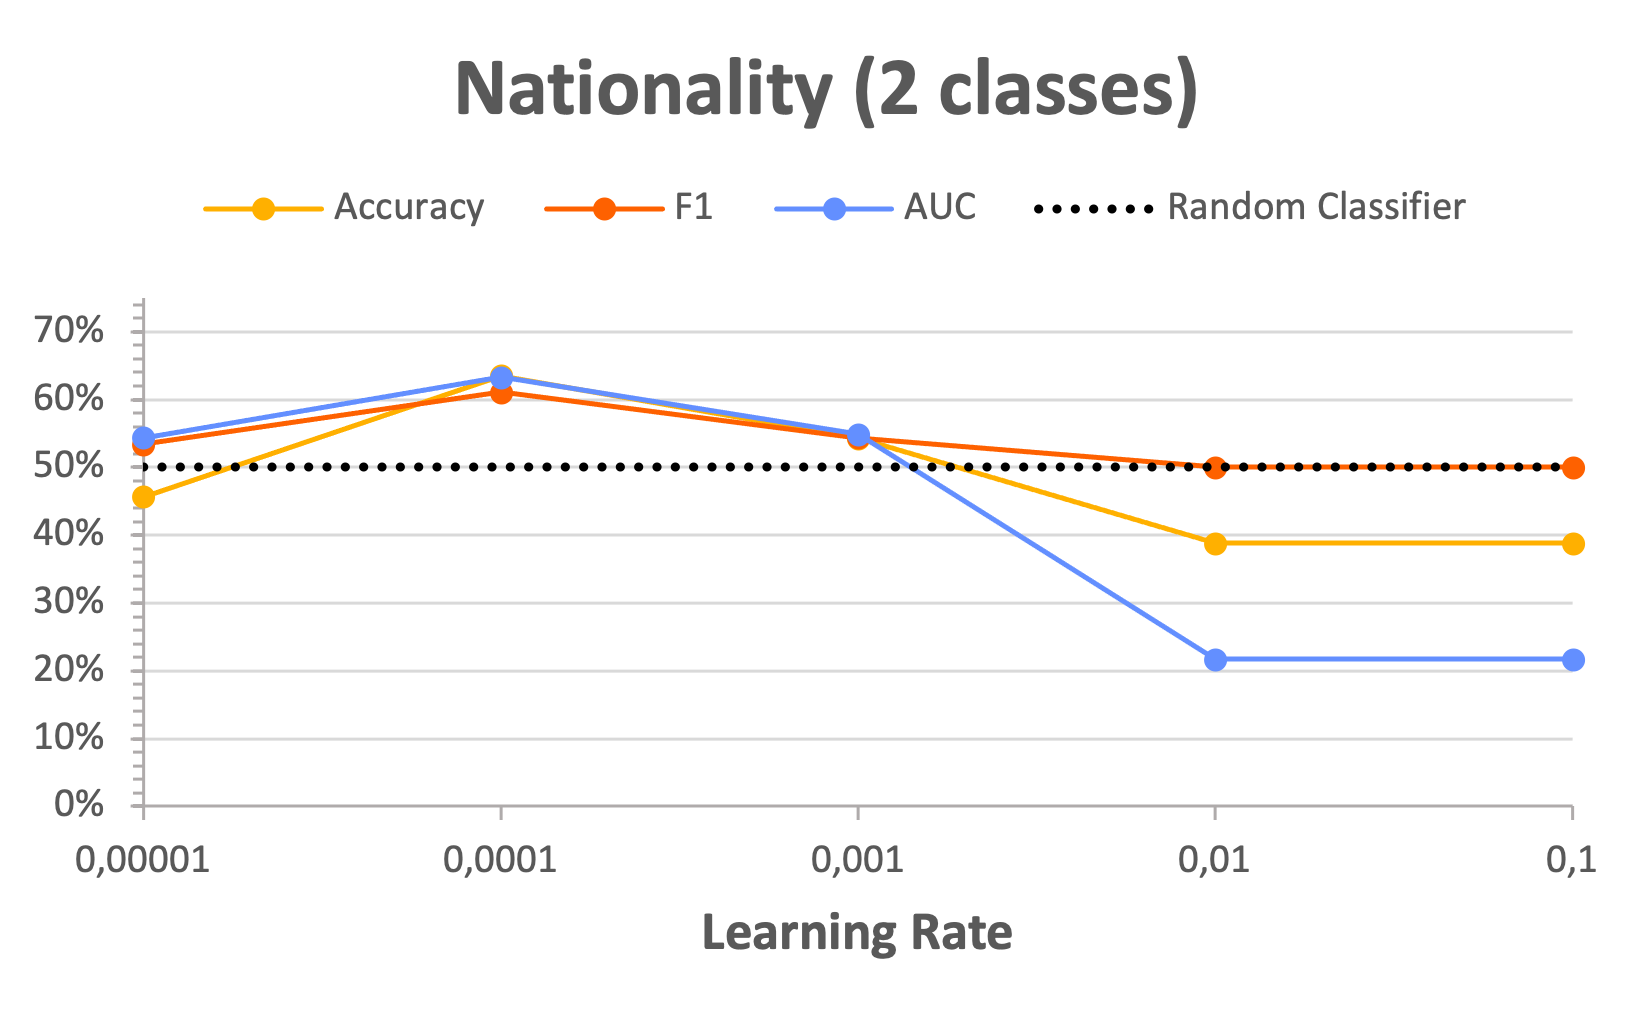
\includegraphics[width=\textwidth]{plots/lr_nat.png}
         \caption{Learning Rate}
         \label{fig:lr_nat}
     \end{subfigure}

    \caption{Predicting the user's nationality from swiped words trajectories.}
    \label{fig:nat}
\end{figure}

% For the nationality target \autoref{fig:nat}, with 2 classes a random classifier's accuracy is 50\%. Whereas, the best performance accuracy achieved in our experiments is 63,50\% with the configuration: RNN, 2 hidden layers, 150 hidden units and a learning rate of 10$^{-4}$.

\begin{figure}[]
     \centering
     \def\w{0.45\linewidth}
     \begin{subfigure}{\w}
         \centering
         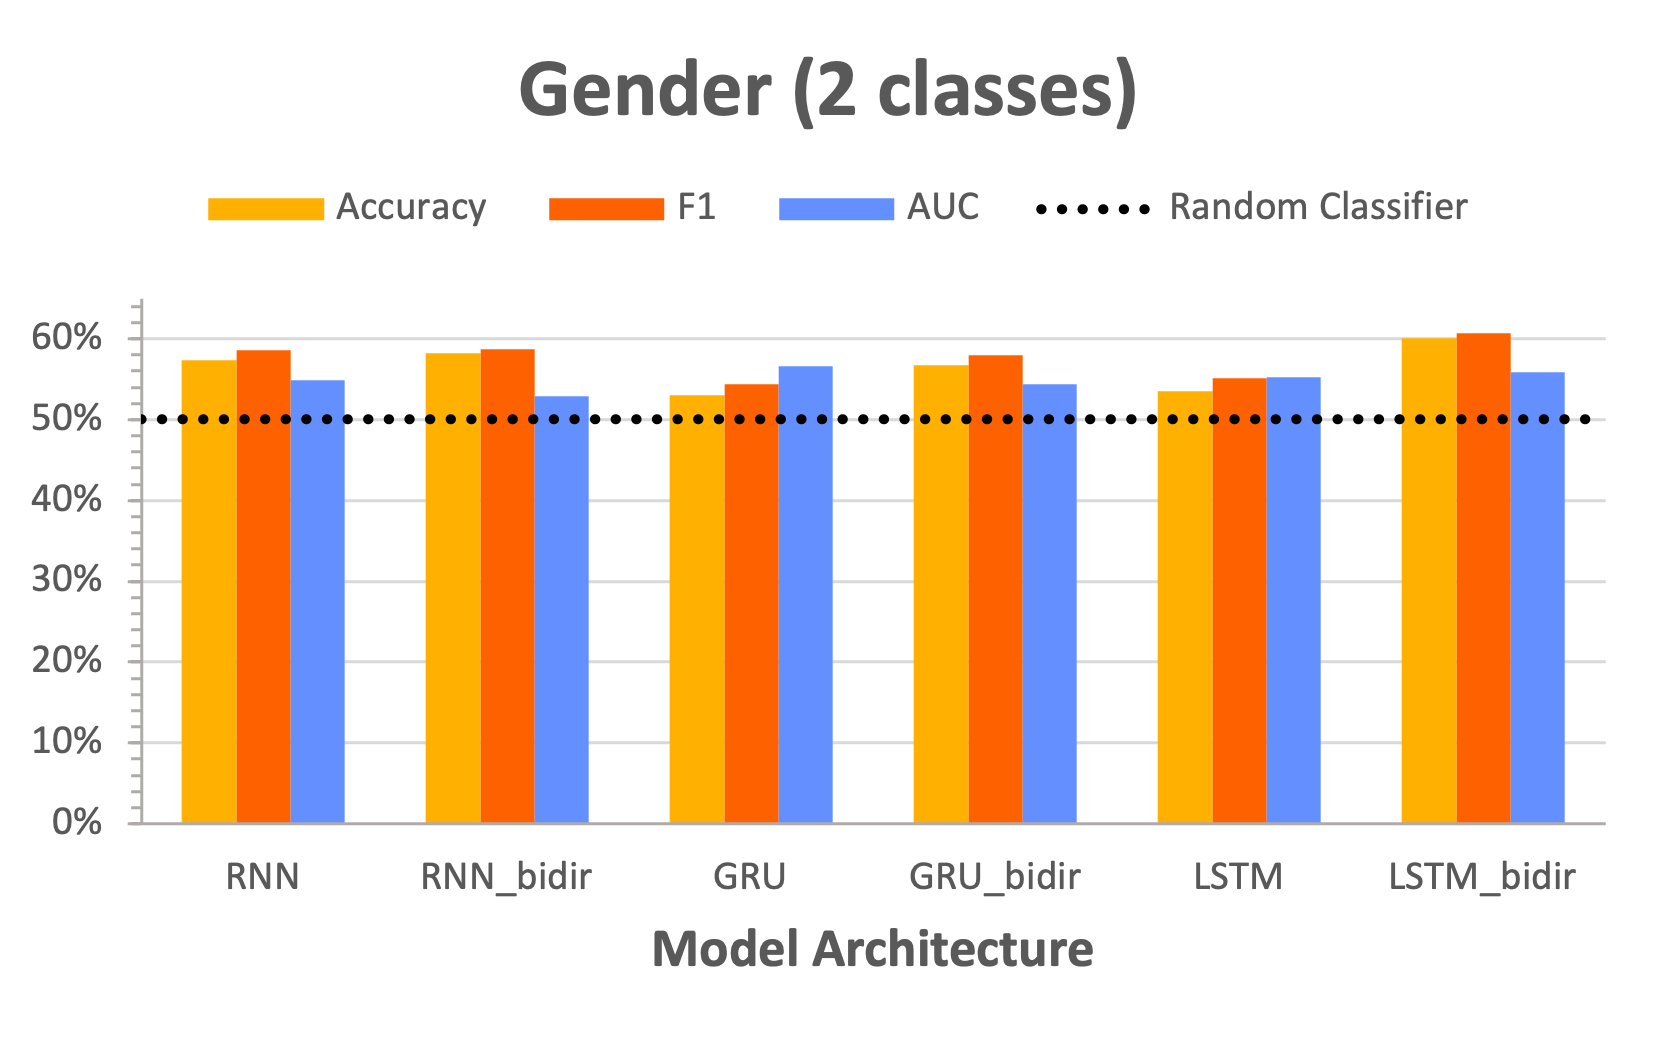
\includegraphics[width=\textwidth]{plots/model_gender.png}
         \caption{Layer type}
         \label{fig:models_gender}
     \end{subfigure}
     \hfill
     \begin{subfigure}{\w}
         \centering
         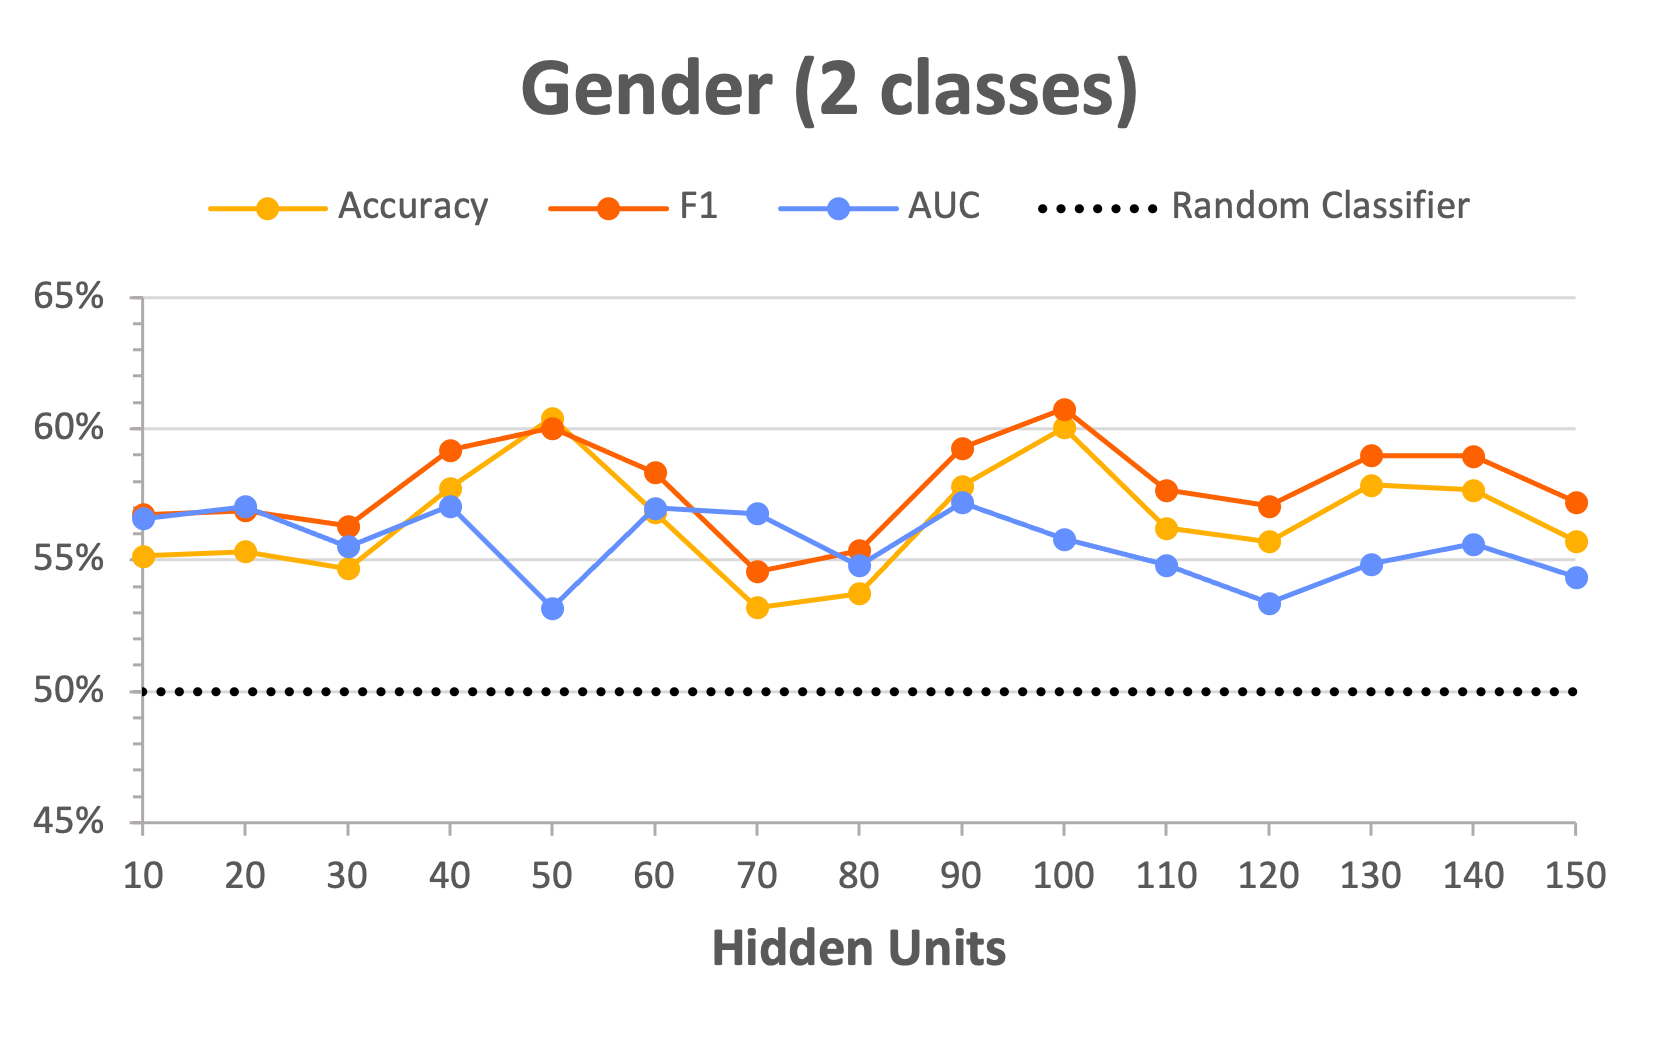
\includegraphics[width=\textwidth]{plots/units_gender.png}
         \caption{Hidden Units}
         \label{fig:units_gender}
     \end{subfigure}\\
     \begin{subfigure}{\w}
         \centering
         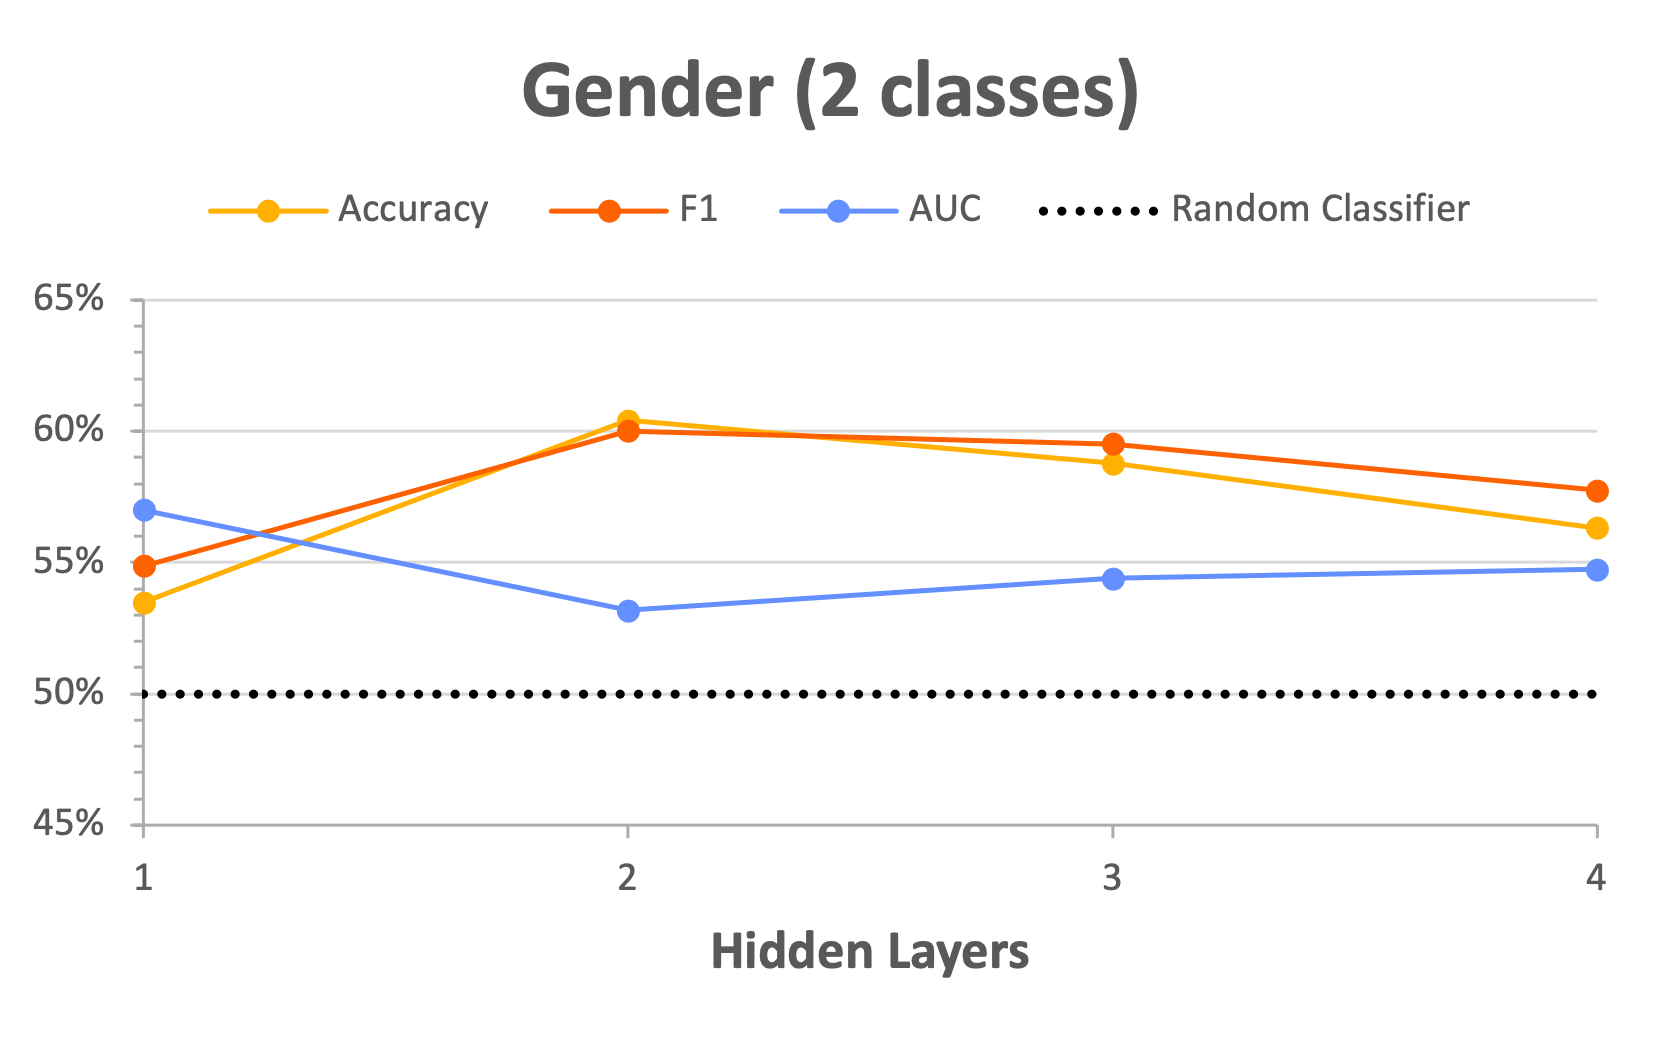
\includegraphics[width=\textwidth]{plots/layers_gender.png}
         \caption{Hidden Layers}
         \label{fig:layers_gender}
     \end{subfigure}
     \hfill
     \begin{subfigure}{\w}
         \centering
         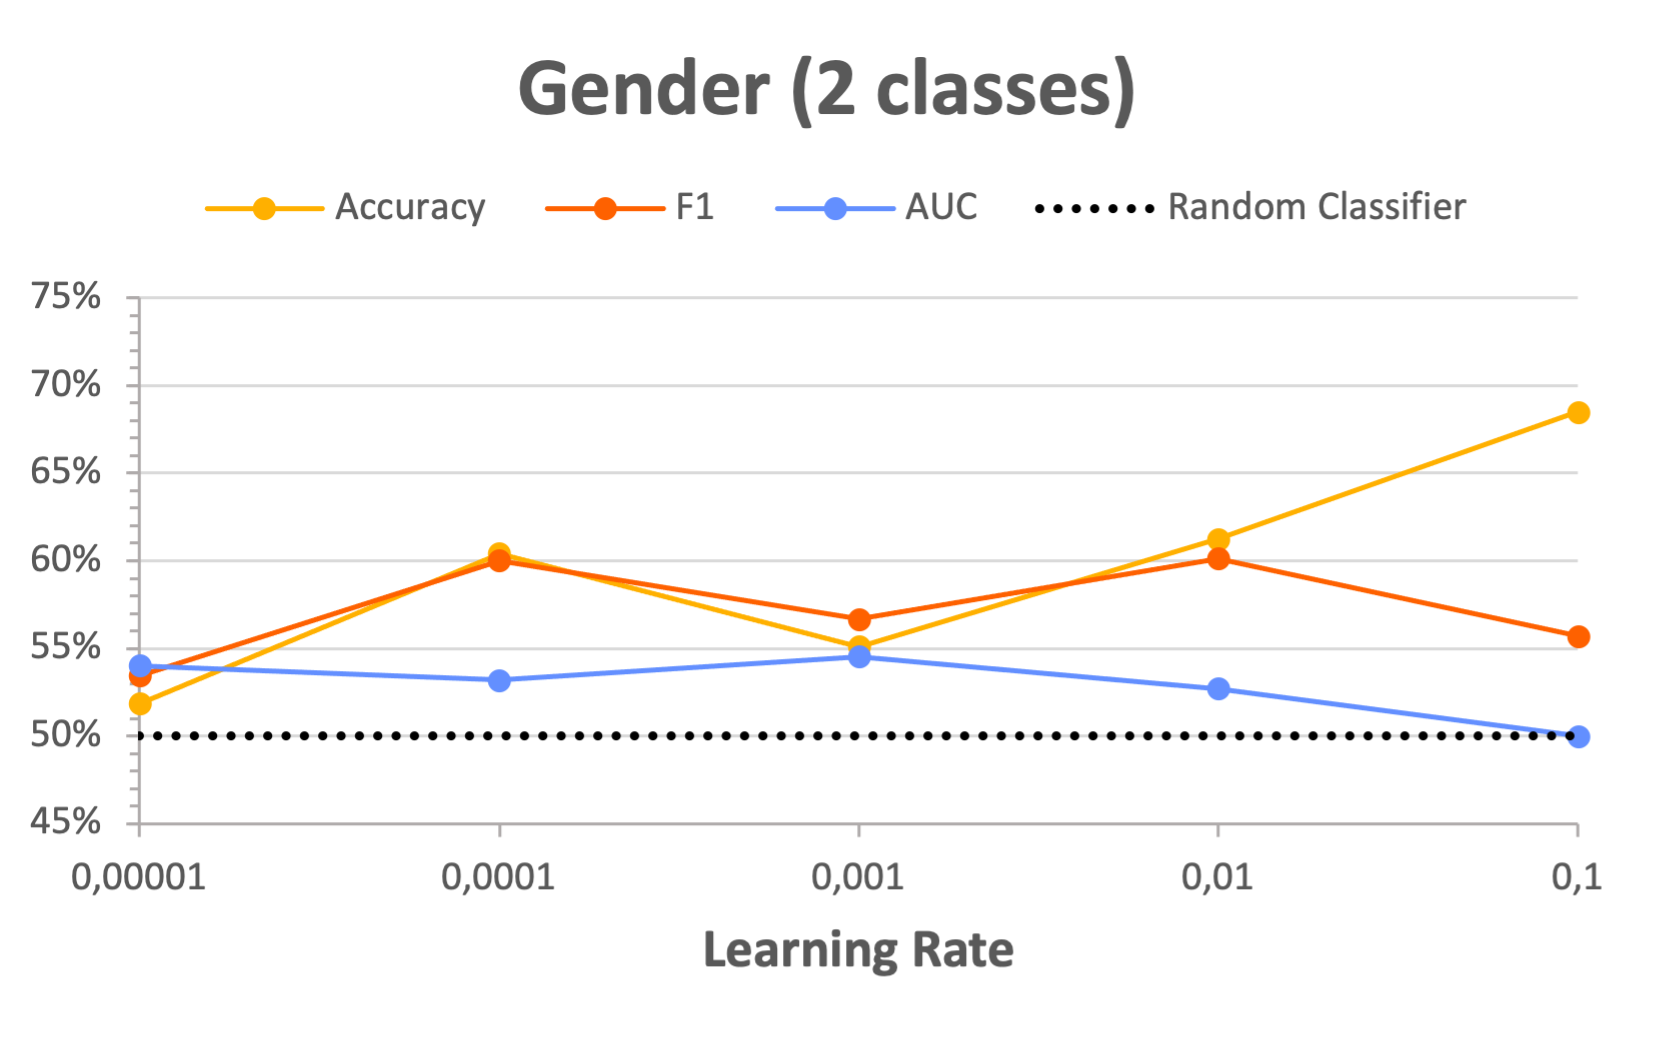
\includegraphics[width=\textwidth]{plots/lr_gender.png}
         \caption{Learning Rate}
         \label{fig:lr_gender}
     \end{subfigure}

    \caption{Predicting the user's gender from swiped words trajectories.}
    \label{fig:gender}
\end{figure}

% For the gender target in \autoref{fig:gender}, with 2 classes a random classifier's accuracy is 50\%. The best performance accuracy achieved in our experiments is 68,51\% with the configuration BiLSTM model, 2 hidden layers, 50 hidden units and a learning rate of 10$^{-1}$.

\begin{figure}[]
     \centering
     \def\w{0.45\linewidth}
     \begin{subfigure}{\w}
         \centering
         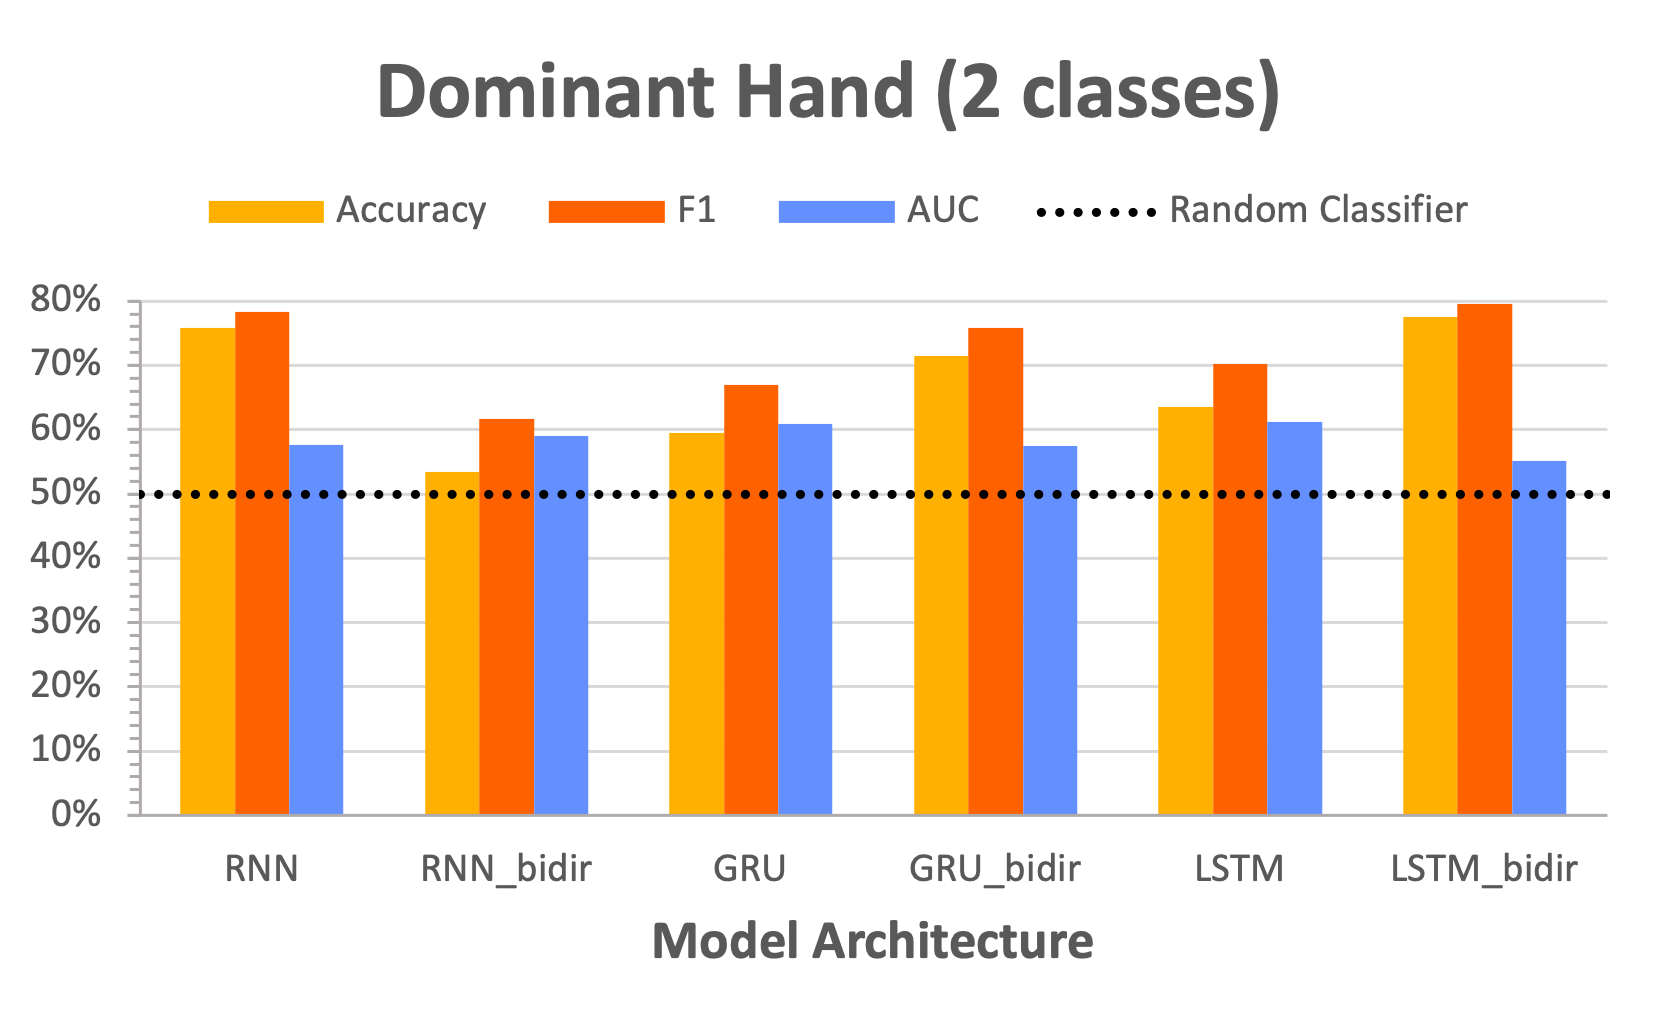
\includegraphics[width=\textwidth]{plots/model_dom.png}
         \caption{Layer type}
         \label{fig:models_dom}
     \end{subfigure}
     \hfill
     \begin{subfigure}{\w}
         \centering
         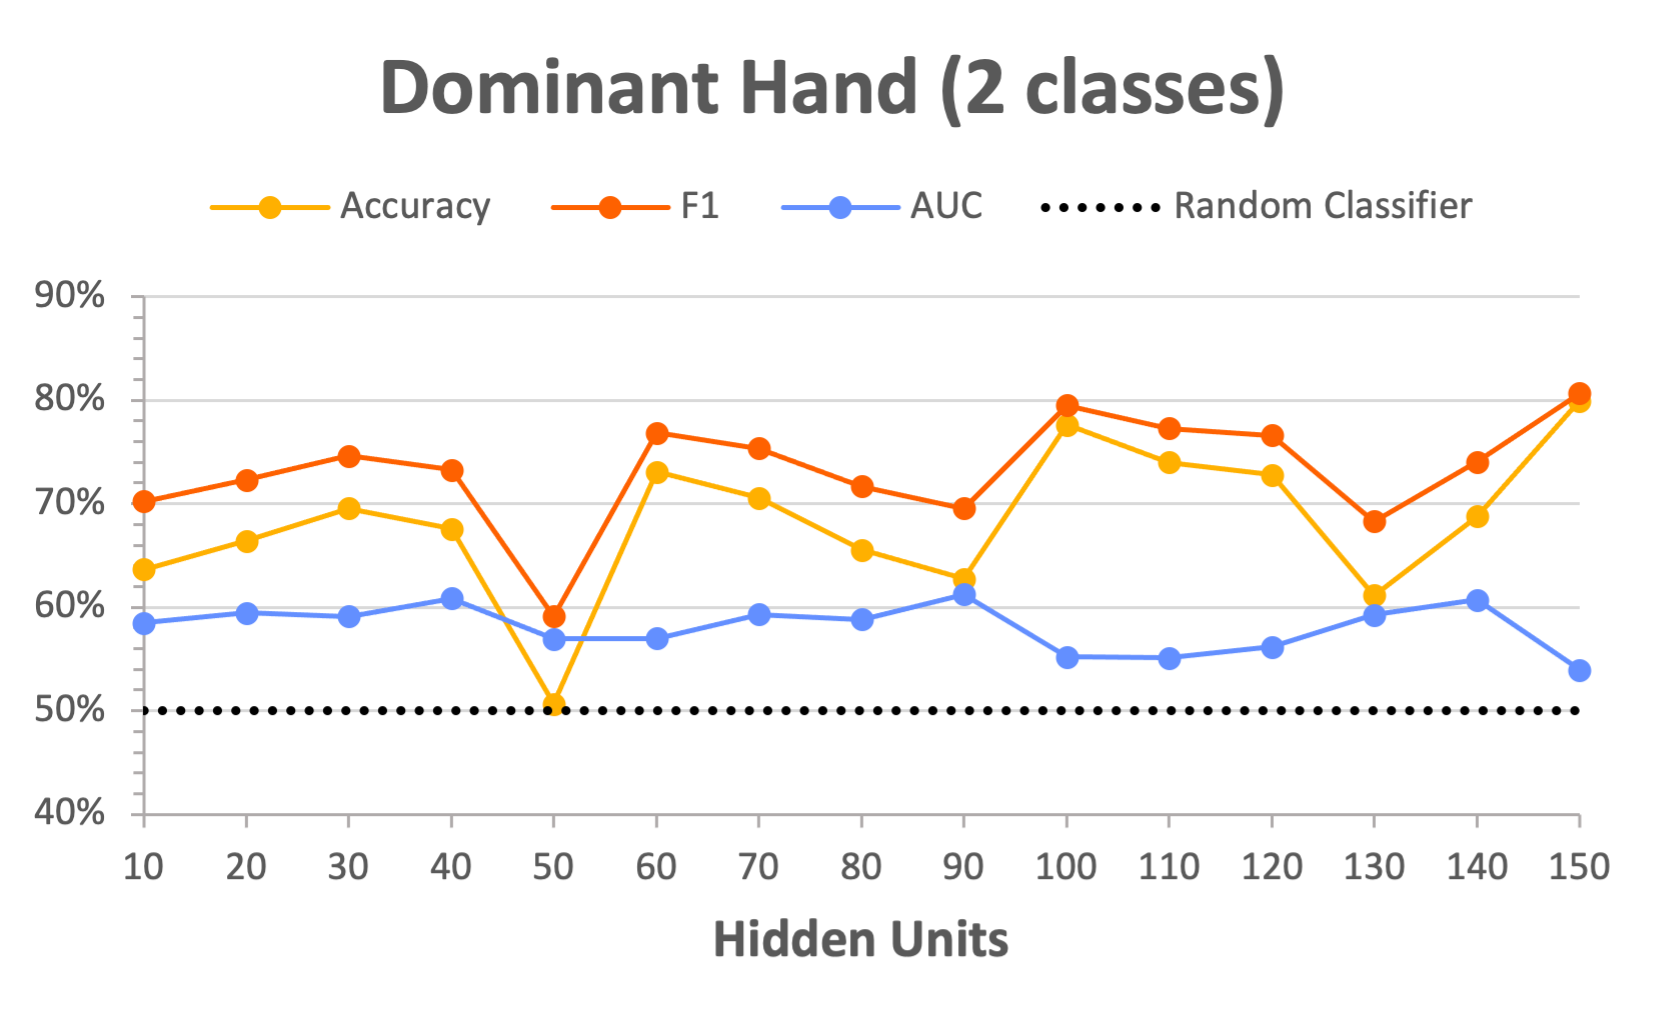
\includegraphics[width=\textwidth]{plots/units_dom.png}
         \caption{Hidden Units}
         \label{fig:units_dom}
     \end{subfigure}\\
     \begin{subfigure}{\w}
         \centering
         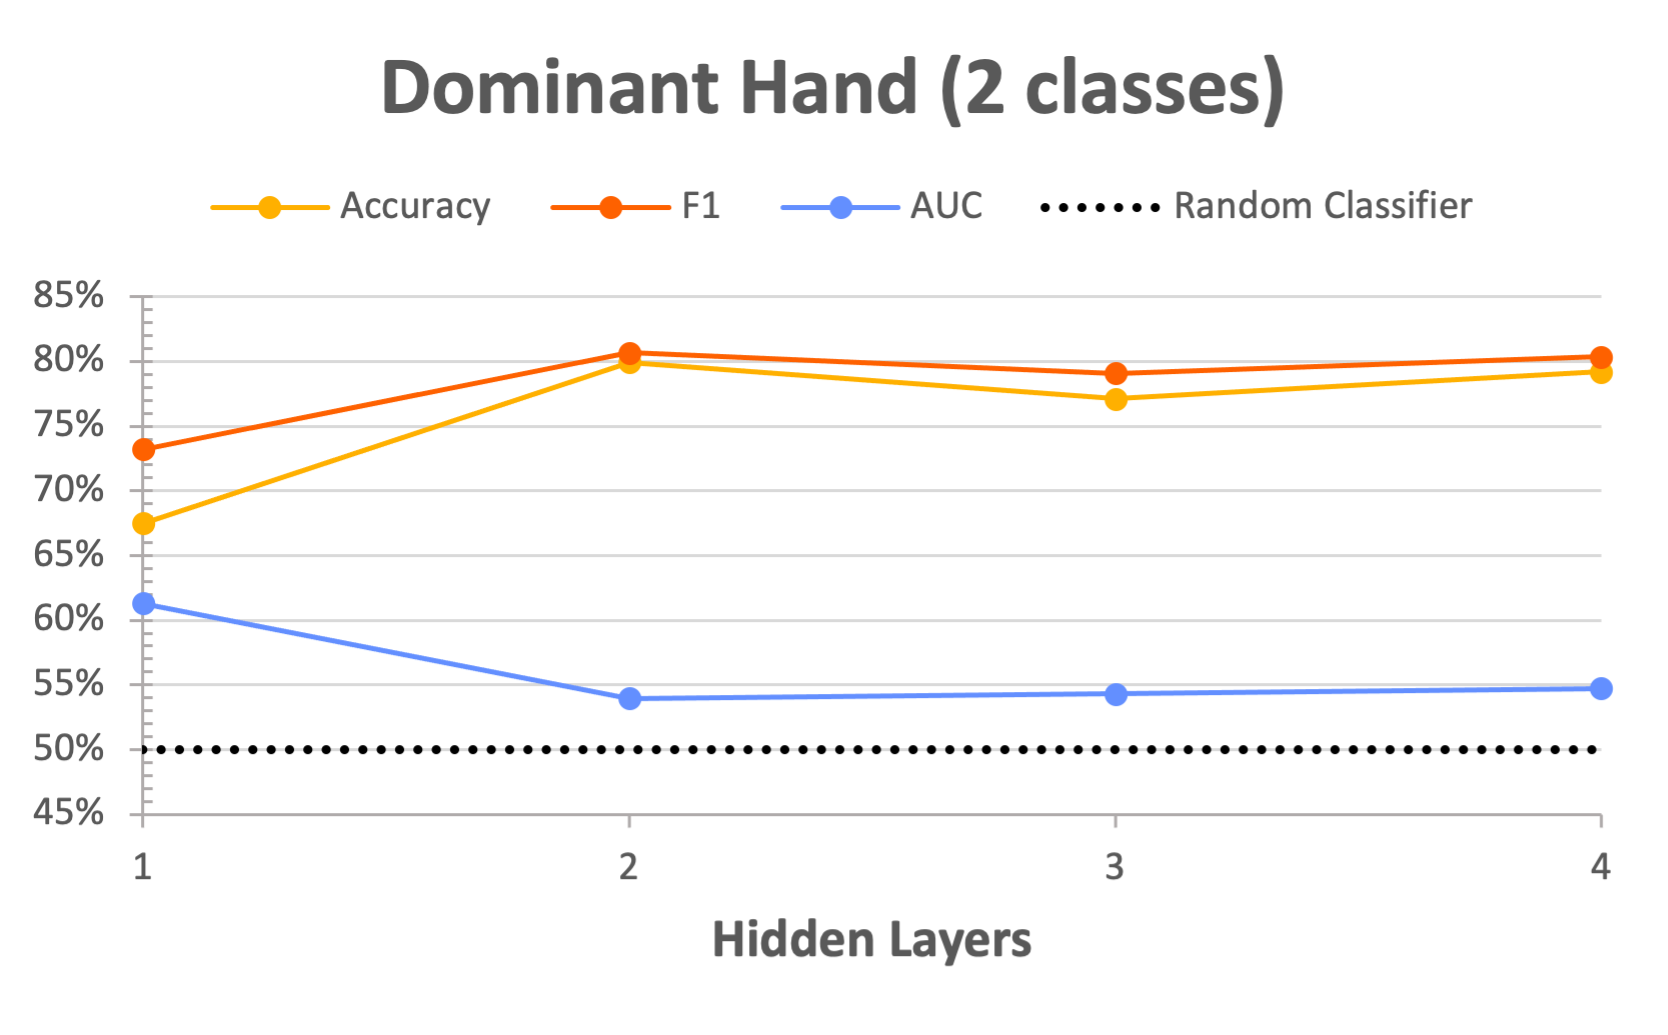
\includegraphics[width=\textwidth]{plots/layers_dom.png}
         \caption{Hidden Layers}
         \label{fig:layers_dom}
     \end{subfigure}
     \hfill
     \begin{subfigure}{\w}
         \centering
         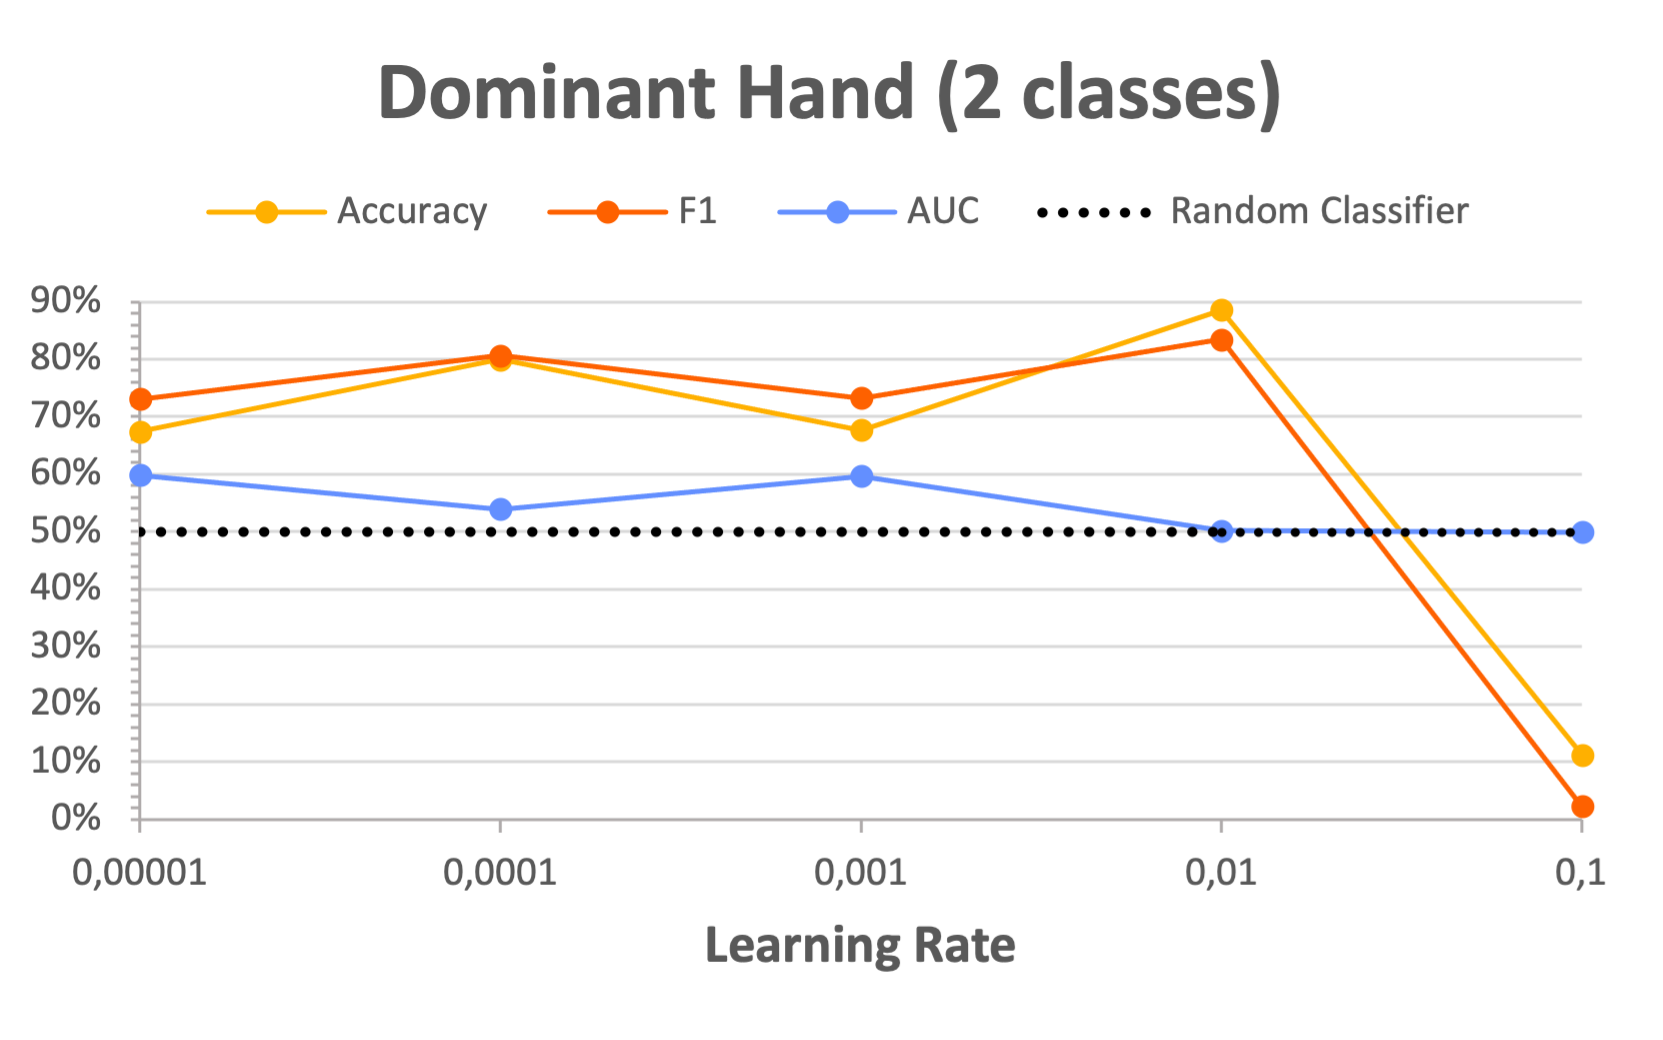
\includegraphics[width=\textwidth]{plots/lr_dom.png}
         \caption{Learning Rate}
         \label{fig:lr_dom}
     \end{subfigure}

    \caption{Predicting the user's dominant hand from swiped words trajectories.}
    \label{fig:dom}
\end{figure}

% For the dominant hand target in \autoref{fig:dom}, with 2 classes the accuracy of a random classifier is 50\%. The best performance accuracy achieved in our experiments is 88,57\% with  the configuration BiLSTM model, 2 hidden layers, 150 hidden units and a learning rate of 10$^{-2}$.

\begin{figure}[]
     \centering
     \def\w{0.45\linewidth}
     \begin{subfigure}{\w}
         \centering
         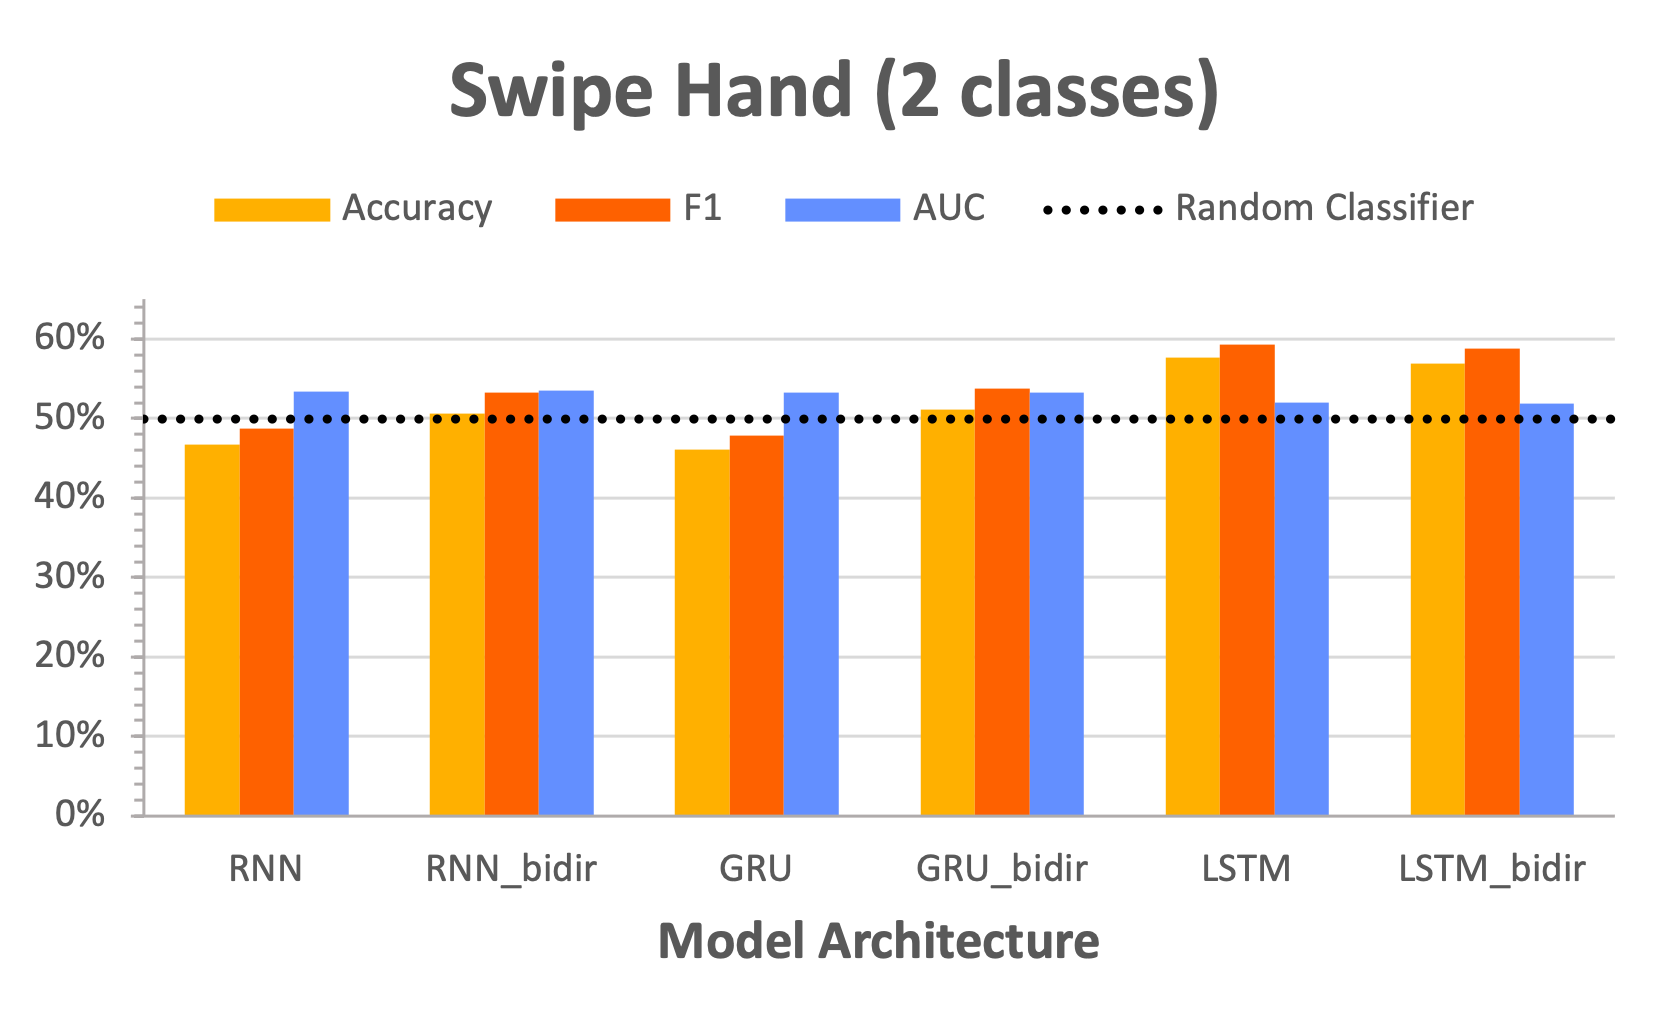
\includegraphics[width=\textwidth]{plots/model_hand.png}
         \caption{Layer type}
         \label{fig:models_hand}
     \end{subfigure}
     \hfill
     \begin{subfigure}{\w}
         \centering
         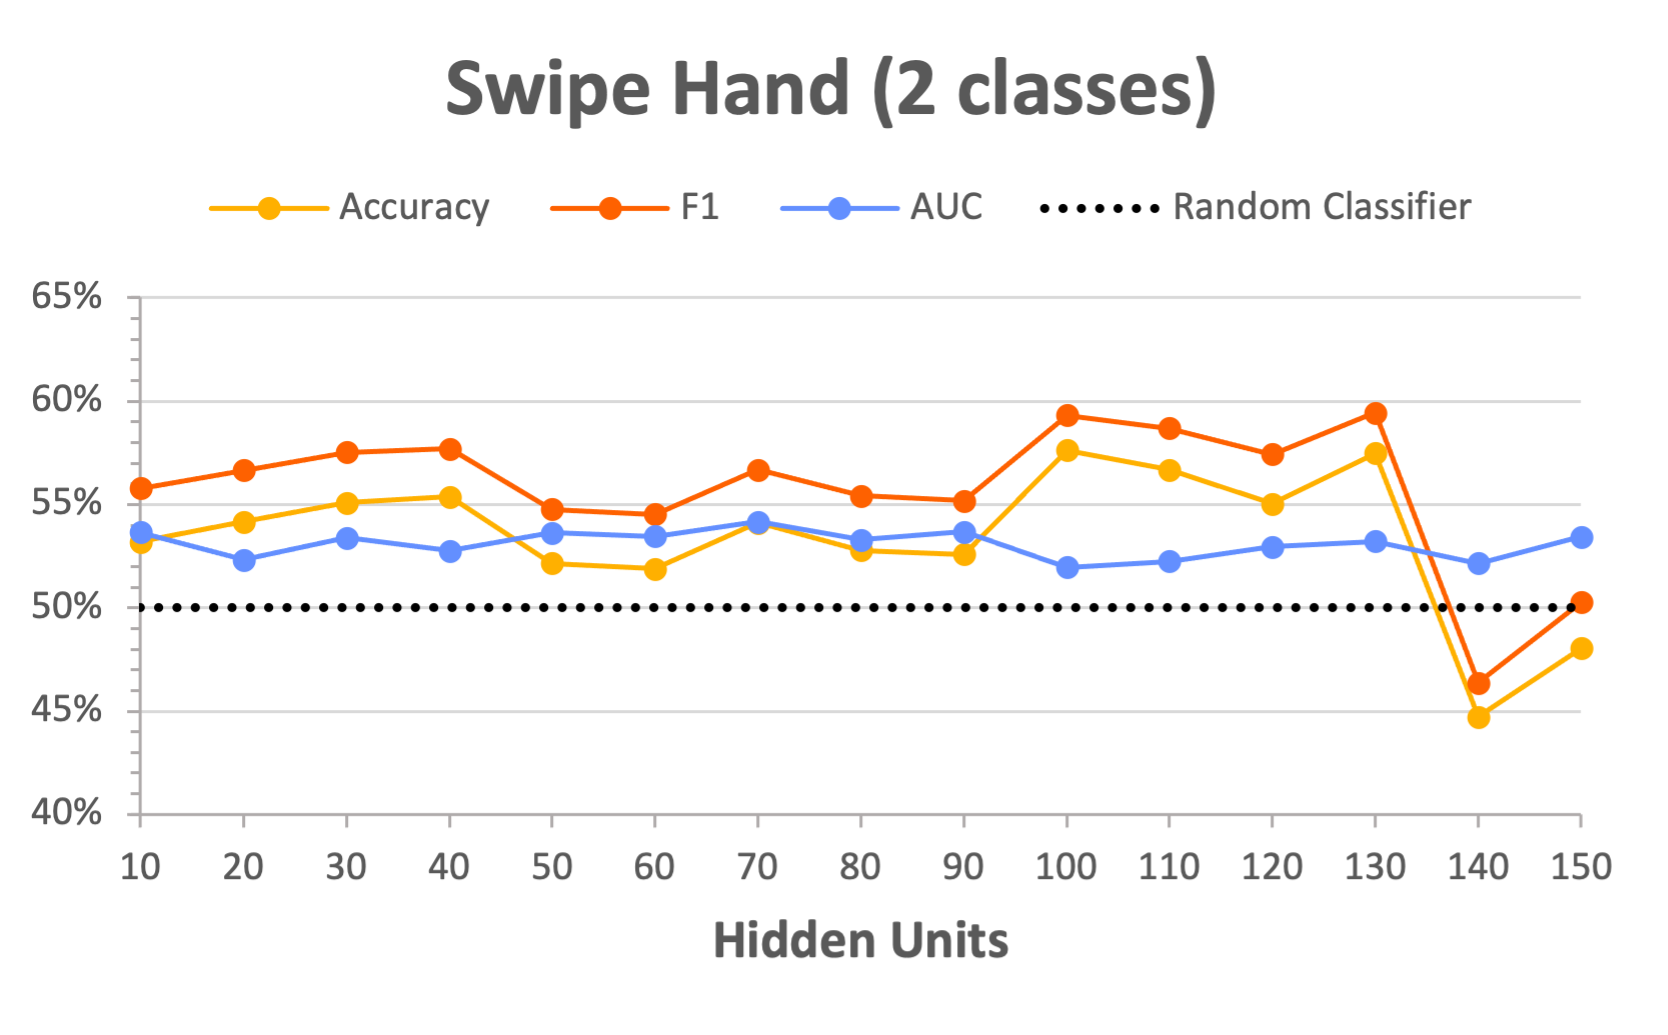
\includegraphics[width=\textwidth]{plots/units_hand.png}
         \caption{Hidden Units}
         \label{fig:units_hand}
     \end{subfigure}\\
     \begin{subfigure}{\w}
         \centering
         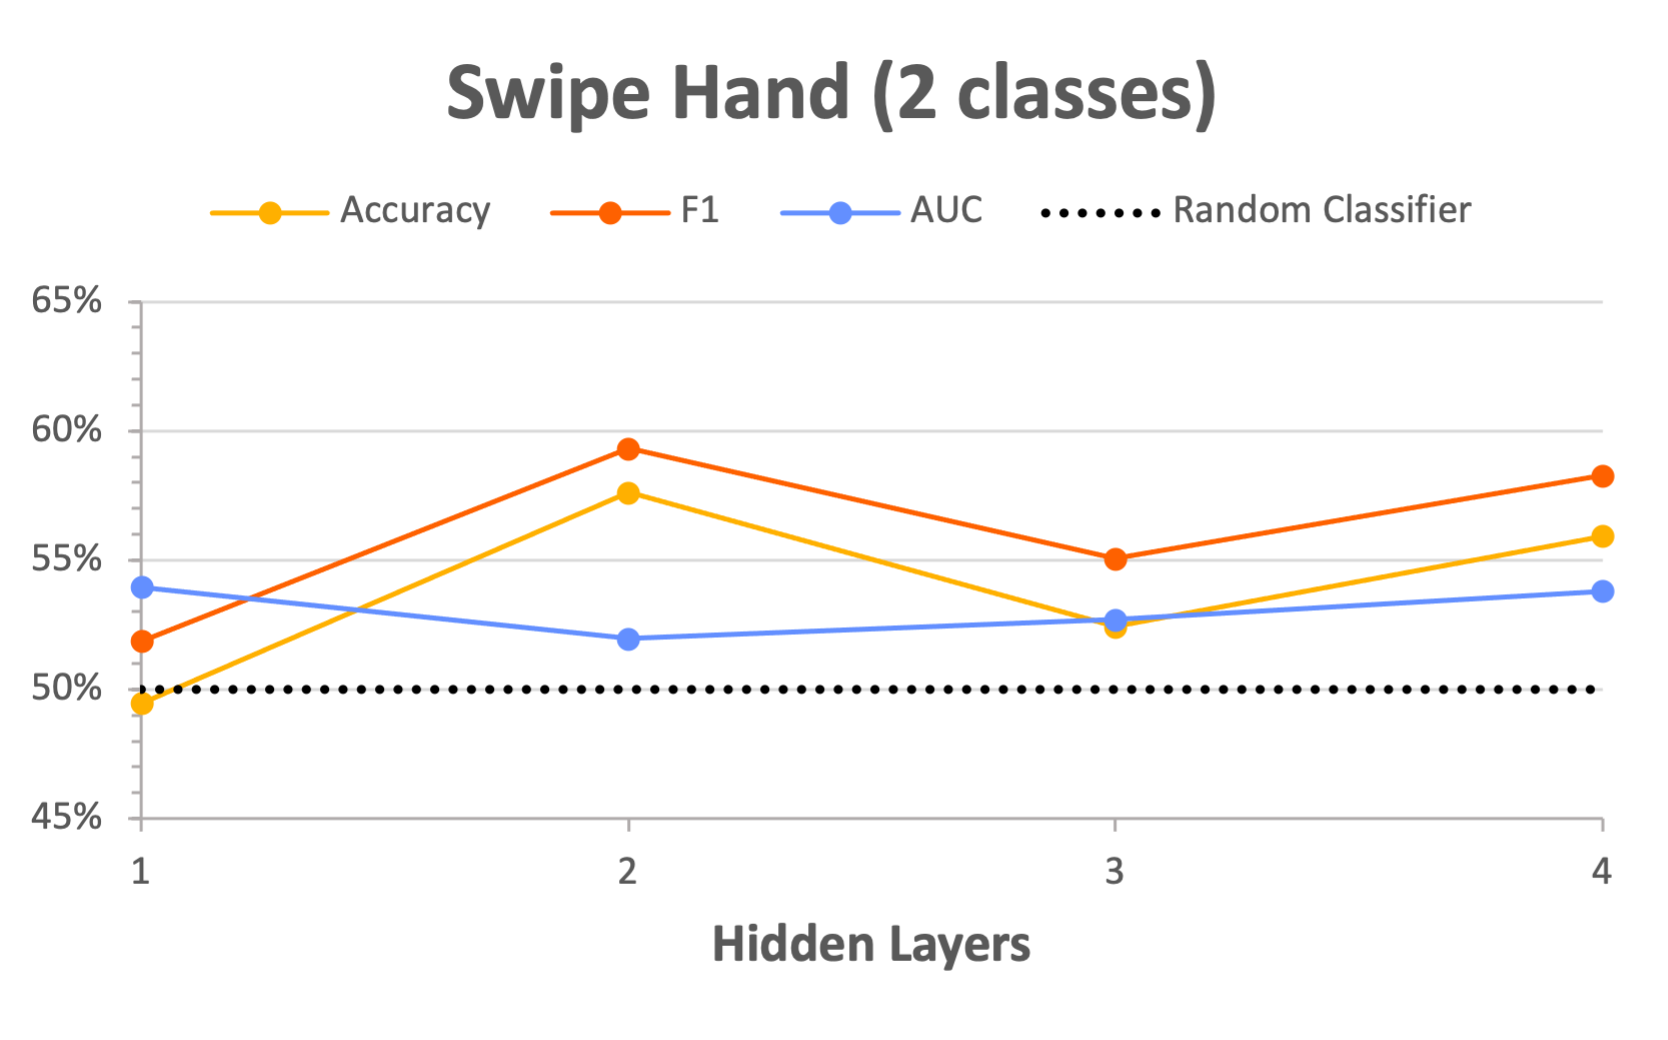
\includegraphics[width=\textwidth]{plots/layers_hand.png}
         \caption{Hidden Layers}
         \label{fig:layers_hand}
     \end{subfigure}
     \hfill
     \begin{subfigure}{\w}
         \centering
         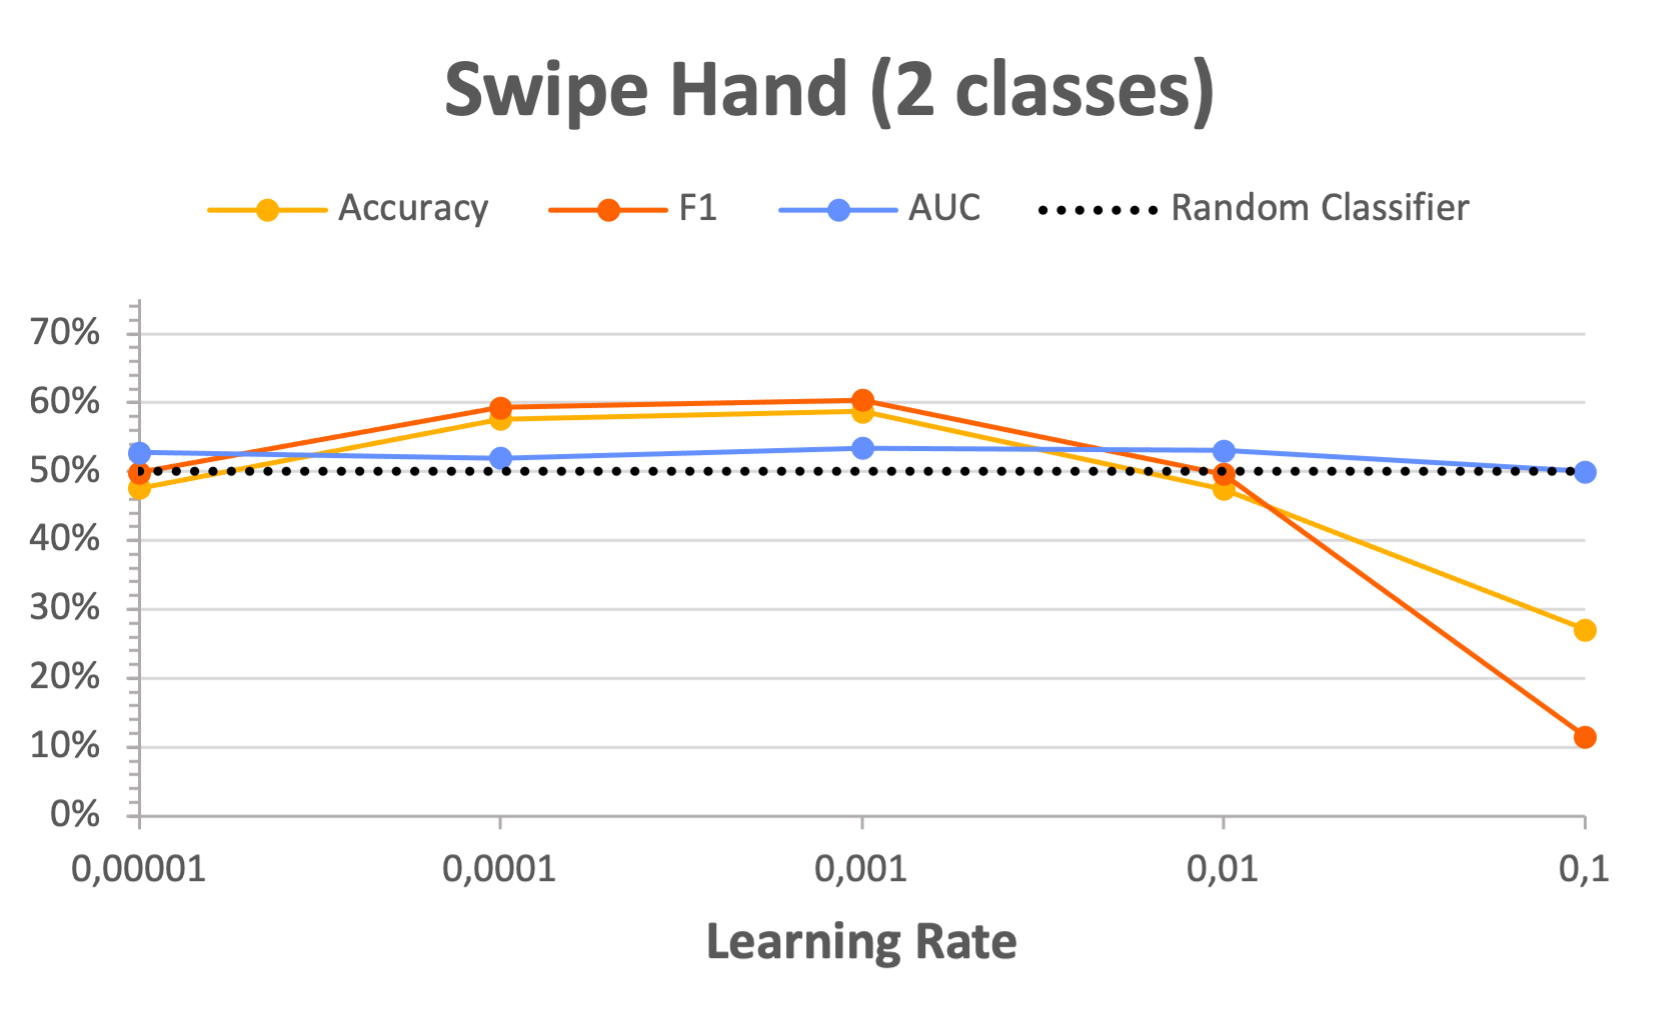
\includegraphics[width=\textwidth]{plots/lr_hand.png}
         \caption{Learning Rate}
         \label{fig:lr_hand}
     \end{subfigure}

    \caption{Predicting the user's swiping hand from swiped words trajectories.}
    \label{fig:hand}
\end{figure}

% For the swiping hand target in \autoref{fig:hand}, with 2 classes a random classifier's accuracy is 50\%. The best performance accuracy achieved in our experiments is 58,74\% with the configuration: LSTM model, 2 hidden layers, 100 hidden units and a learning rate of 10$^{-3}$.

\begin{figure}[]
     \centering
     \def\w{0.45\linewidth}
     \begin{subfigure}{\w}
         \centering
         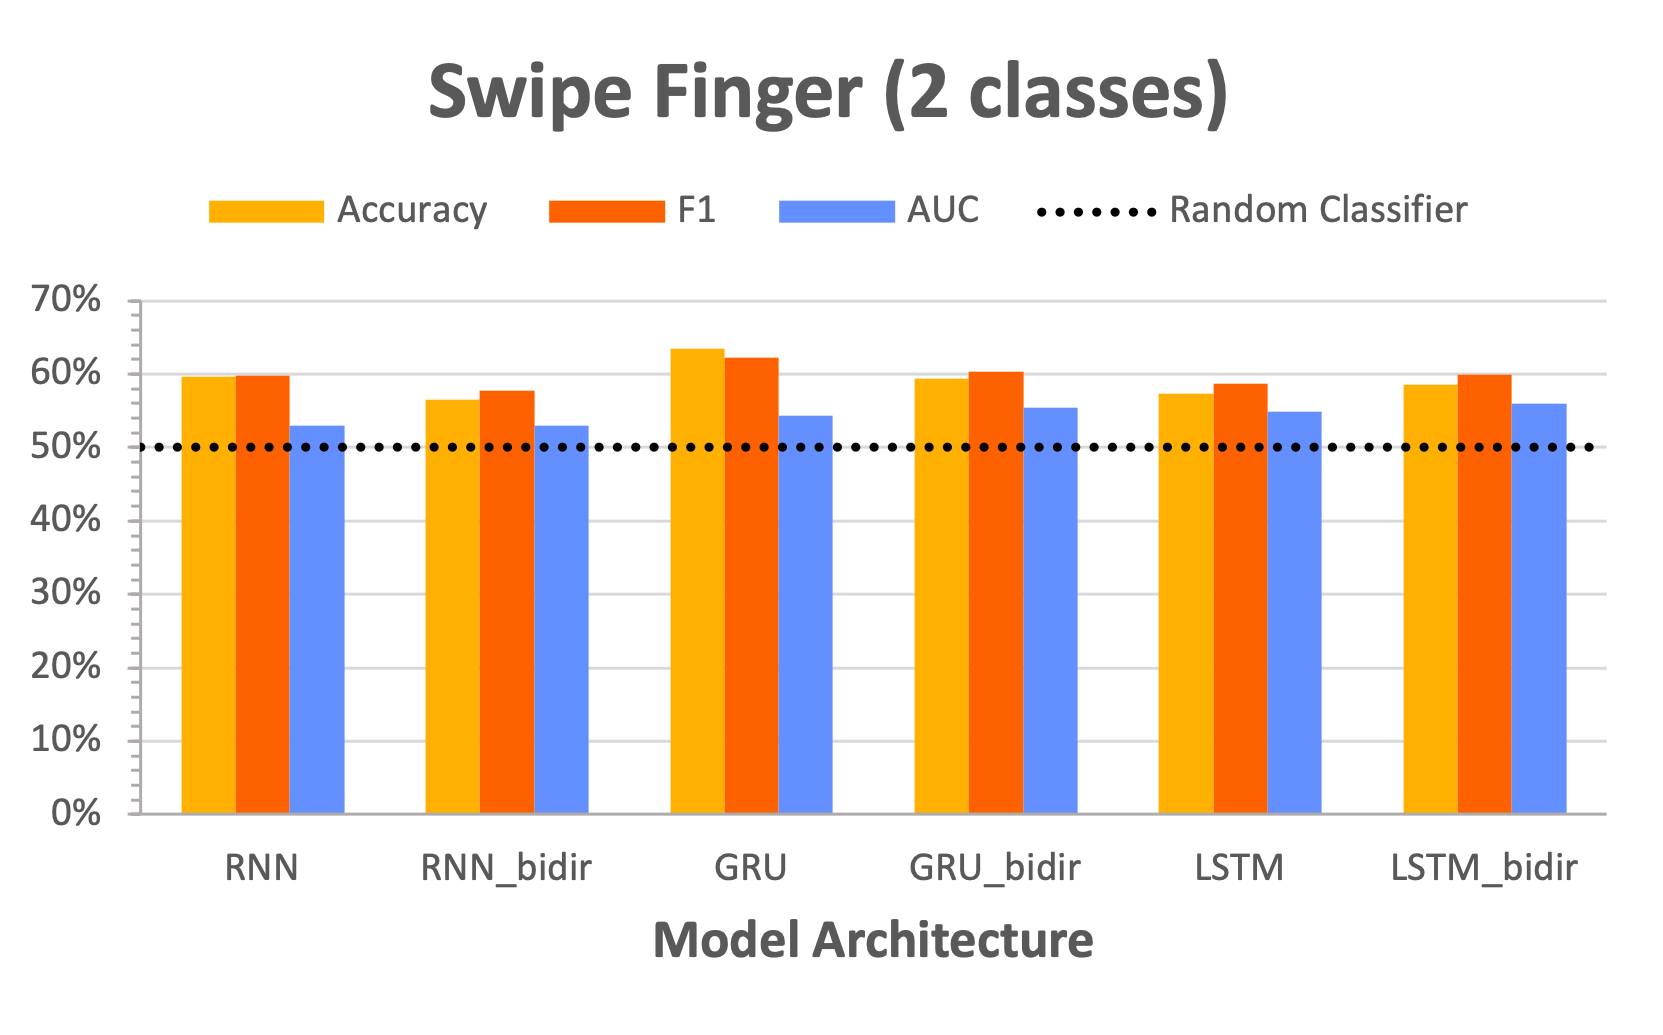
\includegraphics[width=\textwidth]{plots/model_finger.png}
         \caption{Layer type}
         \label{fig:models_finger}
     \end{subfigure}
     \hfill
     \begin{subfigure}{\w}
         \centering
         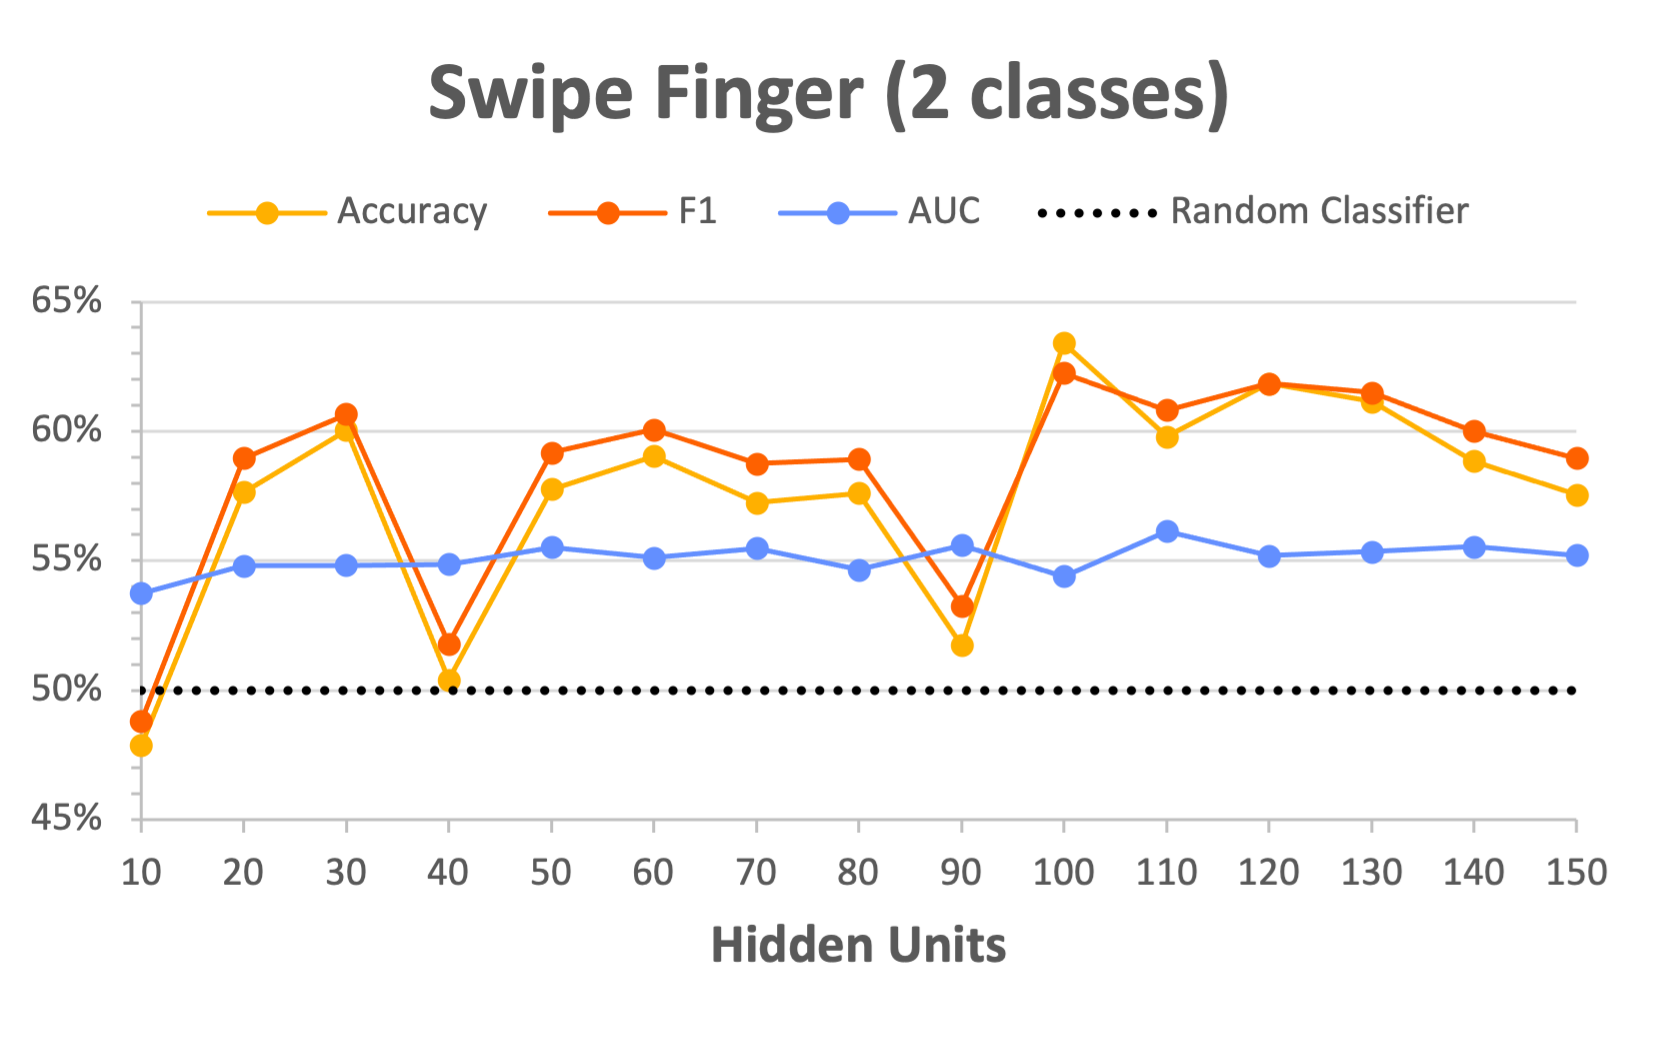
\includegraphics[width=\textwidth]{plots/units_finger.png}
         \caption{Hidden Units}
         \label{fig:units_finger}
     \end{subfigure}\\
     \begin{subfigure}{\w}
         \centering
         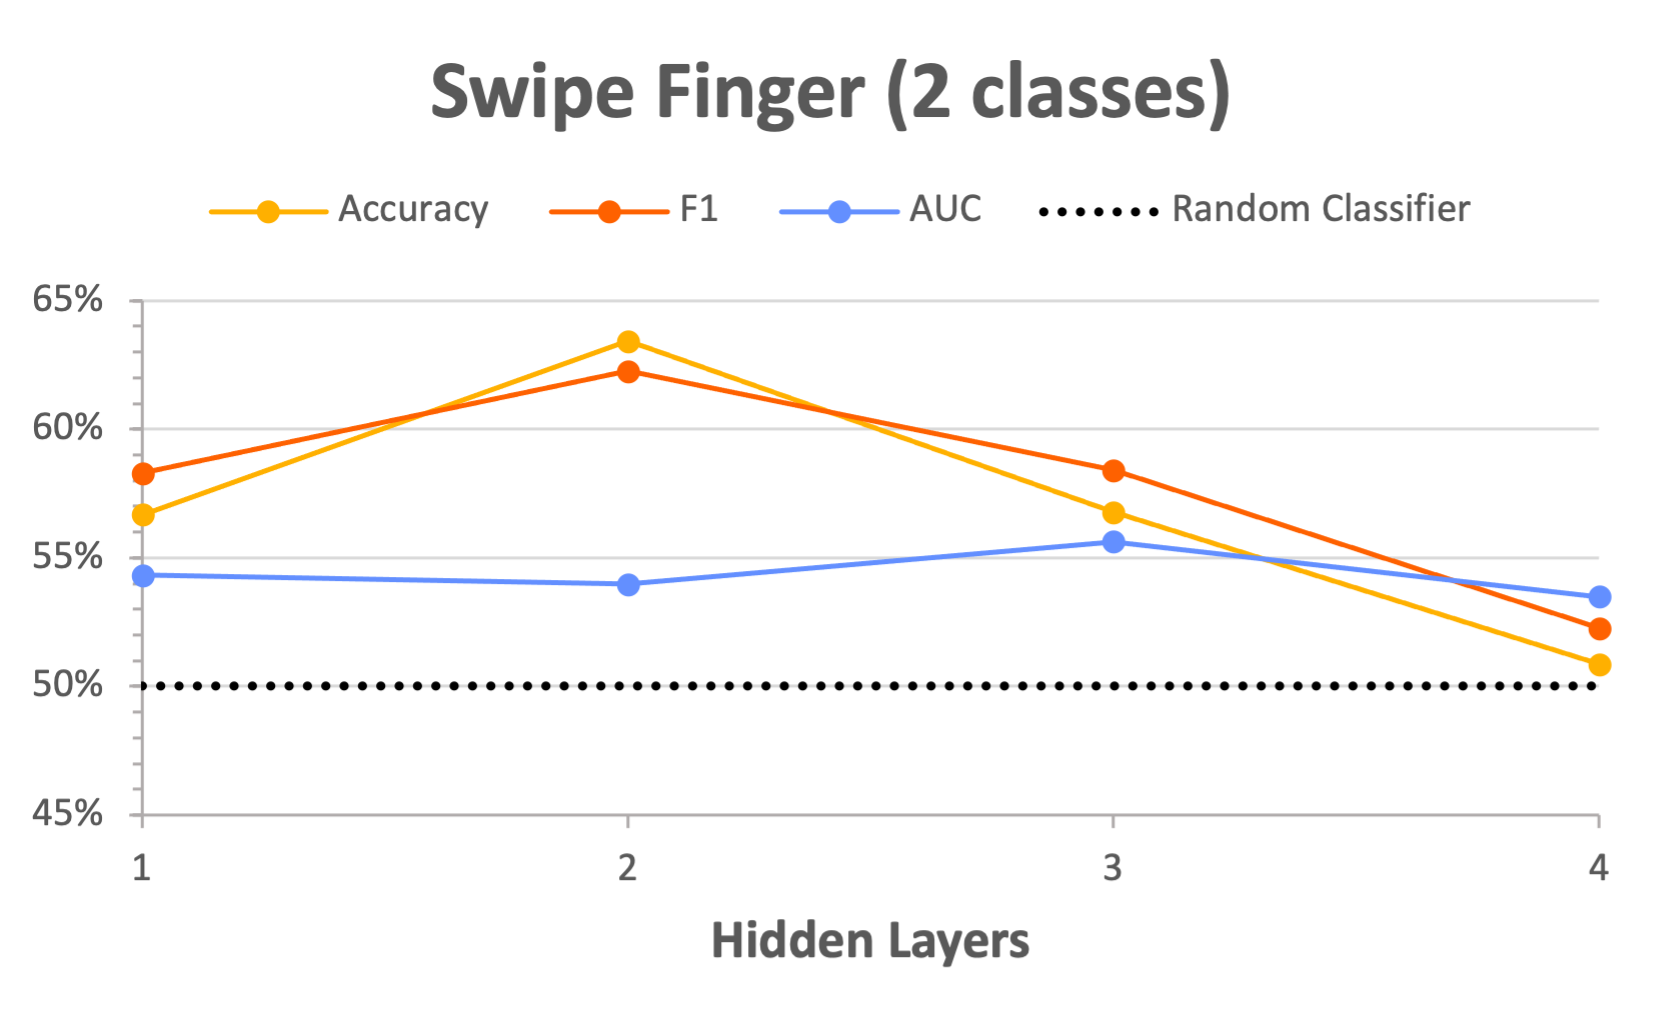
\includegraphics[width=\textwidth]{plots/layers_finger.png}
         \caption{Hidden Layers}
         \label{fig:layers_finger}
     \end{subfigure}
     \hfill
     \begin{subfigure}{\w}
         \centering
         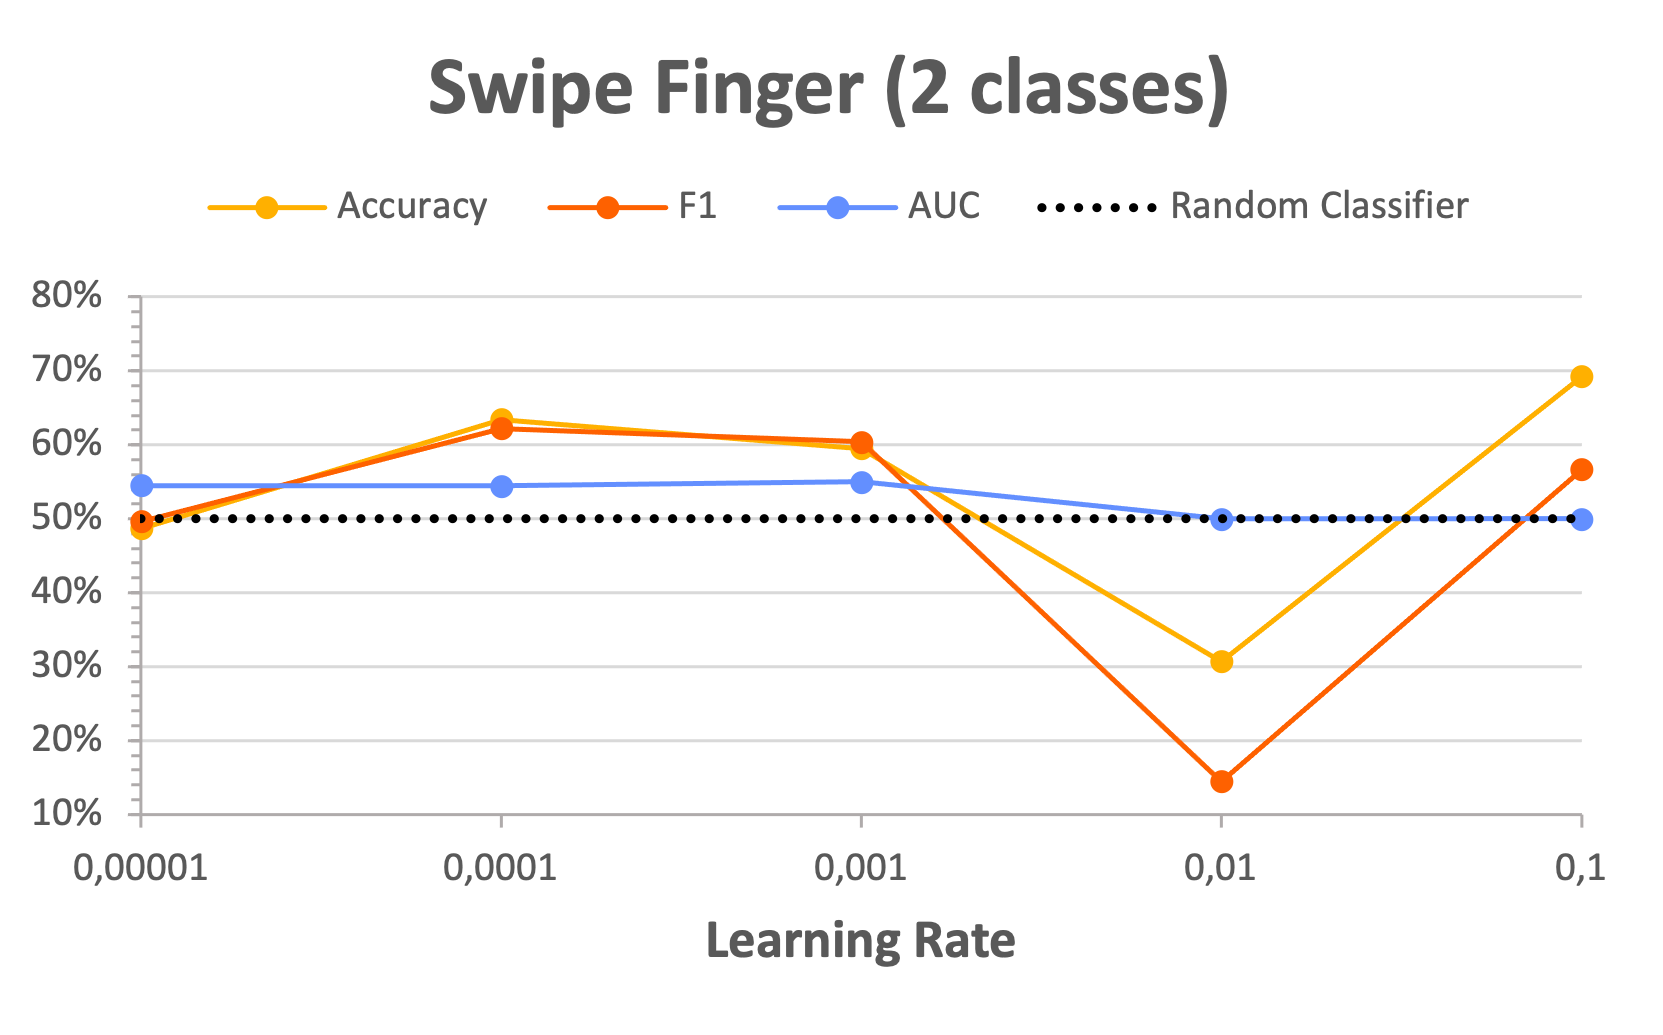
\includegraphics[width=\textwidth]{plots/lr_finger.png}
         \caption{Learning Rate}
         \label{fig:lr_finger}
     \end{subfigure}

    \caption{Predicting the user's swiping finger from swiped words trajectories.}
    \label{fig:finger}
\end{figure}

% For the swiping finger target in \autoref{fig:finger}, with 2 classes a random classifier's accuracy is 50\%. The best performance accuracy achieved in our experiments is 69,28\% with the configuration: GRU model, 2 hidden layers, 100 hidden units and a learning rate of 10$^{-1}$.

\autoref{tab:Results} summarizes the best performing models and their corresponding hyperparameters.
We also provide a random classifier baseline to contextualize the importance of the results.
As shown in the table, the classifiers performed best on most demographic and behavioural correlates by defining the model to be bidirectional and choosing recurrent layers with LSTM or GRU cells. All models performed  better than a random classifier, with an increase from 4\% to 10\% for the swiping familiarity, age and swiping hand targets, and with an increase from 10 to almost 40\% for the English level, nationality, gender, dominant hand and swiping finger targets. Overall, our results show that the trained classifiers were able to identify latent demographic traits from the swiping trajectories, hence validating our hypothesis that swiping carries rich information about the user. This opens interesting research avenues which are yet to be fully explored. For example, new techniques to prevent advanced user profiling should be devised in future work.


\begin{table}[!ht]
\centering
\small
\setlength\tabcolsep{0.5em}
\begin{tabular}{ll *5r}
\toprule
\textbf{Target} & \textbf{Model} & \textbf{Layers} & \textbf{Units} & \textbf{LR} & \textbf{Rand. Acc.} & \textbf{Model Acc.} \\
\midrule
Age                 & BiGRU  & 2 & 150 & $10^{-3}$ & 33.33\% & 40.91\% \\
Gender              & BiLSTM & 2 & 50  & $10^{-1}$ & 50\%    & 68.51\% \\
Nationality         & RNN    & 2 & 150 & $10^{-4}$ & 50\%    & 63.50\% \\
\midrule
Familiarity         & LSTM   & 2 & 140 & $10^{-4}$ & 33.33\% & 37.87\% \\
English level       & BiLSTM & 4 & 100 & $10^{-4}$ & 25\%    & 37.32\% \\
Dominant hand       & BiLSTM & 2 & 150 & $10^{-2}$ & 50\%    & 88.57\% \\
Swiping hand        & LSTM   & 2 & 100 & $10^{-3}$ & 50\%    & 58.74\% \\
Swiping finger      & GRU    & 2 & 100 & $10^{-1}$ & 50\%    & 69.28\% \\
\bottomrule
\end{tabular}
\caption{Summary of the best model architectures for predicting demographic (top rows) and behavioral (bottom rows) information from swiping trajectories.}
\label{tab:Results}
\end{table}

\rev{
Finally, we also report the confusion matrices for each of the best performing models in \autoref{fig:confusion_matrices}.
As we can see, in most cases the trained models were able to successfully discriminate between classes.
However, in other cases the models failed to learn properly to discriminate and degenerated as ZeroR classifier,
i.e. a model that always predicts the majority class.
This only happened to the models that predicted gender, dominant hand, and swiping finger.
In any case, the performance of all models is better than that of a random classifier,
therefore we validate our research hypothesis and conclude that, overall,
demographic and behavioral information can be inferred from swiping trajectories.
}

\begin{figure}[!ht]
     \centering
     \def\w{0.3\linewidth}

     \begin{subfigure}{\w}
         \centering
         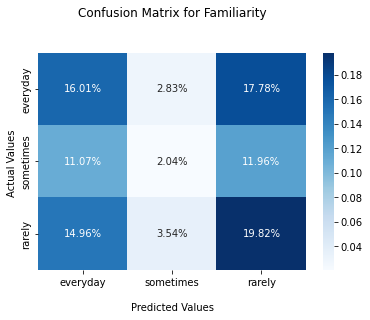
\includegraphics[width=\textwidth]{figures/familiarity_cm.png}
         \caption{\rev{Familiarity}}
         \label{fig:cm_familiarity}
     \end{subfigure}
     \hfill
     \begin{subfigure}{\w}
         \centering
         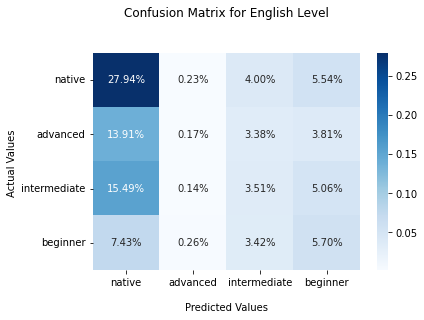
\includegraphics[width=\textwidth]{figures/english_level_cm.png}
         \caption{\rev{English level}}
         \label{fig:cm_engl}
     \end{subfigure}
     \hfill
     \begin{subfigure}{\w}
         \centering
         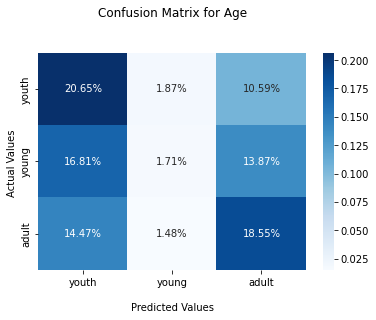
\includegraphics[width=\textwidth]{figures/age_cm.png}
         \caption{\rev{Age}}
         \label{fig:cm_age}
     \end{subfigure}
     \hfill
     \begin{subfigure}{\w}
         \centering
         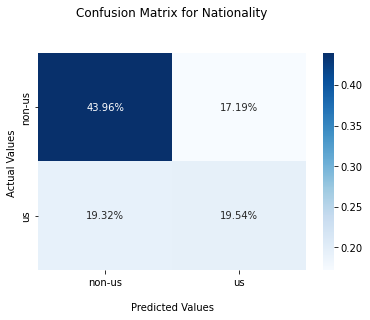
\includegraphics[width=\textwidth]{figures/nationality_cm.png}
         \caption{\rev{Nationality}}
         \label{fig:cm_nat}
     \end{subfigure}
     \hfill
     \begin{subfigure}{\w}
         \centering
         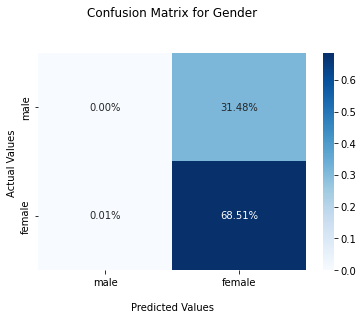
\includegraphics[width=\textwidth]{figures/gender_cm.png}
         \caption{\rev{Gender}}
         \label{fig:cm_gender}
     \end{subfigure}
     \hfill
     \begin{subfigure}{\w}
         \centering
         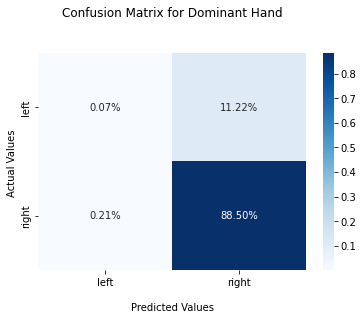
\includegraphics[width=\textwidth]{figures/dominant_hand_cm.png}
         \caption{\rev{Dominant hand}}
         \label{fig:cm_dom}
     \end{subfigure}
     \hfill
     \begin{subfigure}{\w}
         \centering
         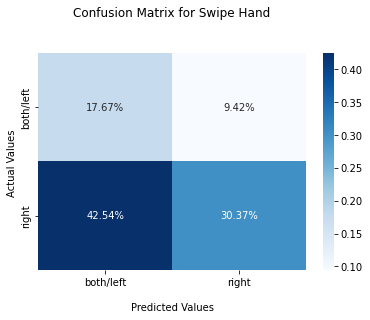
\includegraphics[width=\textwidth]{figures/swipe_hand_cm.png}
         \caption{\rev{Swiping hand}}
         \label{fig:cm_hand}
     \end{subfigure}
     \hfill
     \begin{subfigure}{\w}
         \centering
         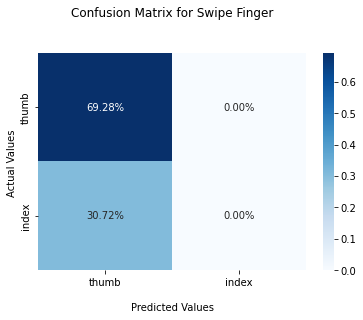
\includegraphics[width=\textwidth]{figures/swipe_finger_cm.png}
         \caption{\rev{Swiping finger}}
         \label{fig:cm_fingder}
     \end{subfigure}
     \hfill
     %% This is to force left-alignment of the last subplot.
     \phantom{
         \begin{subfigure}{\w}
             \centering
             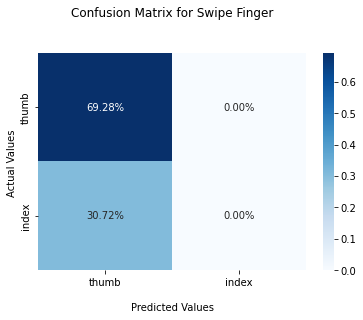
\includegraphics[width=\textwidth]{figures/swipe_finger_cm.png}
             \caption{\rev{Swiping finger}}
             \label{fig:cm_fingder}
         \end{subfigure}
     }

    \caption{\rev{Confusion matrices for the best performing models reported in \protect\autoref{tab:Results}.}}
    \label{fig:confusion_matrices}
\end{figure}



%% ============================================================================
\section{Limitations and Future Work}
\label{sec:limitations}
%% ============================================================================

%% Provide a high-level discussion of the results?
%% What have we learned?
%% What is the takeaway message?
%% What are the limitations of our study?
%% What should be done in the future?

In this work we have focused on single-word classification,
which is the most challenging scenario since some words might be as short as two characters
and therefore the information a classifier can infer is minimal.
It would be interesting to predict demographic and behavioral attributes
at the sentence level, i.e., by considering all swiped words a user might enter in a row.
This could be done\rev{, e.g.,} by concatenating the feature vectors of each word in the sentence.
\rev{In addition,} we have not considered word difficulty in our analysis.
This might be an interesting avenue for future work,
since it has been shown that experienced shape-writing users
tend to be more loose while entering non-familiar words~\cite{Leiva21_swipe}.
It may be the case, therefore, that other demographic and behavioral traits
are highly correlated with swiping patterns.
For example, ageing is marked by a decline in motor control abilities, which is reflected by the users' writing performance.
Smith et al.~\cite{Smith1999} observed that older people incurred in longer movement times,
but also more sub-movements and more pointing errors than the young.
Unfortunately, we cannot study this effect in the dataset we have analyzed,
since most users are aged between 20 and 40 years.
More concretely, the dataset is skewed towards young female right-handed participants.

Our sequence models are \rev{relatively} costly to train
because of their recurrent nature and the large amount of swiping data we analyzed.
For example, training the non-bidirectional LSTM models took between 1.5 to 10 hours
in the High-Performance Computing facilities of our university,
whereas the same model with bidirectional layers took between 3 and 20 hours.
While these training times might be small for today's standards,
real-time processing is clear out of reach at present,
which means that we cannot build our models as new data come in.
\rev{
We also have not experimented with attention mechanisms such as local~\cite{Bahdanau15} and global~\cite{Luong15} attention.
Attention has been proved to be effective for recurrent models,
but we decided to go for an initial exploration of the feasibility of our approach in the first place.
Given that our results are promising, we can even experiment with other architectures such as Transformers in future work.
}
%% TODO: Use Transformers for time series classification:
%% There was a paper about this topic but it's paywalled and it's unclear how it works.

Furthermore, we have explored sequential models only,
as they are better suited to handle the sequential nature of \rev{swipe} trajectories.
Observing the promising results obtained in our study, we believe that other data representations should be explored.
For example, if we consider images (pixel values) instead of discrete spatio-temporal time series as input data,
then we could try Convolutional Neural Networks (CNNs) as well as more powerful architectures like Vision Transformers (ViT).
This is left as an interesting opportunity for future work.

\rev{
Another interesting opportunity for future work is to consider more balanced splits of the data.
Given the number of target classes, there are 1152 possible combinations,
not all of which may be well represented, and are certainly not represented equally.
We should point out, however, that our study is the first to use the original ``How we Swipe'' dataset
for training Machine Learning models and to get a more realistic estimate of their performance.
We also have not considered any interactions between targets, such as gender and age.
For example, training only for young females (which happens to be the most represented group of participants)
might result in more accurate models.
}

Finally, we should remark that all mobile vendors provide a swiping service to millions of users.
Although, they ask for consent to track swiping information for the purpose of improving the service and enhancing user experience,
our study brings to light that extracting personal information of users from swiping data is also within reach.
The significantly large amount of swiping data mobile vendors can have access to,
allows them to build a powerful demographic and behavioral inference engines.
Thus, the users can potentially give up their privacy, without actually consenting to it,
only by sharing their swiping information with mobile vendors.


%% ============================================================================
\section{Conclusion}
\label{sec:conclusion}
%% ============================================================================
%% Summarize in 1 or 2 paragraphs this work.
%% Restate again (but briefly) the main contributions.
%% Conclude with a sentence that provides a broader perspective of this work.

We have analyzed the dynamics of swiping trajectories from the only publicly available swiping dataset
to model and predict different demographic and behavioural correlates.
We explored three popular sequence model architectures (RNN, LSTM, GRU)
and conducted a systematic analysis regarding which model hyperparameters yield better classification performance.
Overall, the classifiers performed best on most demographic and behavioural traits
by defining the models to be bidirectional and choosing recurrent layers with LSTM or GRU cells \rev{having 100 units each}.
\rev{We noticed that the eight considered targets are challenging to predict, however}
the results from our experimental evaluations demonstrate that all models perform better than a random classifier,
with an increase from 4 to 10\% for the swiping familiarity, age, and swiping hand targets,
and with an increase from 10 to 40\% for the English level, nationality, gender, dominant hand, and swiping finger targets.
\rev{For the three latter targets (gender, dominant hand, and swiping finger)
the trained models tended to predict the majority class.}

Taken together, our results show that the classifiers are able to identify latent demographic and behavioral information from swiping trajectories,
hence validating our research hypothesis that swiping carries rich information about the user.
This \rev{finding} may have unexpected consequences for user's privacy,
since currently swiping is supported by all mobile vendors and has millions of users,
so people may be inadvertently profiled at an unprecedented granularity.
\rev{It is a matter of time for researchers to build more sophisticated Machine Learning models, therefore}
future work should consider new ways of addressing these issues without impacting the user's swiping experience.

\backmatter

\bmhead{Acknowledgements}
The experiments presented in this paper were carried out
using the HPC facilities of the University of Luxembourg: \url{http://hpc.uni.lu}

\section*{Declarations}

\subsection*{Funding}
This work was supported by the Horizon 2020 FET program of the European Union through the ERA-NET Cofund funding grant CHIST-ERA-20-BCI-001 and the European Innovation Council Pathfinder program (SYMBIOTIK project, grant 101071147).

\subsection*{Competing interests}
The authors have no competing interests to declare that are relevant to the content of this article.

\subsection*{Availability of data and materials}
The swiping dataset we used is publicly available at \url{https://osf.io/sj67f/}.

\section*{Authors' contributions}
%% https://www.elsevier.com/authors/journal-authors/policies-and-ethics/credit-author-statement
\textbf{D.C.A. Lemarquis}: Software, Writing - Original Draft.
\textbf{B.A. Yilma}: Methodology, Writing - Original Draft.
\textbf{L.A. Leiva}: Conceptualization, Methodology, Writing - Reviewing and Editing.


%\small
%\bibliographystyle{abbrv}
\bibliography{references}

\end{document}
